\documentclass{article}
\author{Daniel Monjas Migu\'elez 
 		\\ \\ 2 DGIIM Universidad de Granada}
\title{SISTEMAS OPERATIVOS}
\usepackage[utf8]{inputenc}
\usepackage[T1]{fontenc}
\usepackage[spanish,es-tabla]{babel}
\usepackage{graphicx}
\usepackage[hidelinks]{hyperref}
\hypersetup{
	colorlinks=true,
	linkcolor=blue,
	filecolor=magenta,
	urlcolor=cyan,
}

\graphicspath{ {images/} }

\begin{document}
\maketitle
\newpage
\tableofcontents
\newpage
\section{Soporte hardware (	HW) al sistema operativo}
	\subsection{Elementos Básicos}
		Al más alto nivel, un computador consta del procesador, la memoria y los componentes de E/S, incluyendo uno o más módulos de cada tipo. Estos componentes se interconectan de manera que se puede lograr la función principal del computador, que es ejecutar programas. Por tanto hay cautro elementos estructurales principales:
		\begin{itemize}
			\item \textbf{Procesador.} Controla el funcionamiento del computador y realiza sus funciones de procesamiento de datos. Cuando sólo hay un procesador, se denomina Central Processing Unit, CPU.
			\item \textbf{Memoria principal.} Almacena datos y programas. Esta memoria es habitualmente volátil;es decir, cuando se apaga el computador, se pierde su contenido. En contraste, el contenido de la memoria del disco se mantiene incluso cuando se apaga el computador. A la memoria principal se le denomina también memoria real o memoria primaria
			\item \textbf{Módulos de E/S.} Transfieren los datos entre el computador y su entorno externo. El entorno externo está formado por diversos dispositivos, incluyendo dispositivos de memoria secundaria, equipos de comunicaciones y terminales.
			\item \textbf{Bus del sistema.} Proporciona comunicación entre los procesadores, la memoria principal y los módulos de entrada salida
		\end{itemize}
		
		\begin{figure}
			\caption{Componentes de un computador: vision al más alto nivel}
			\label{fig1.1:componentes}
			\centering
			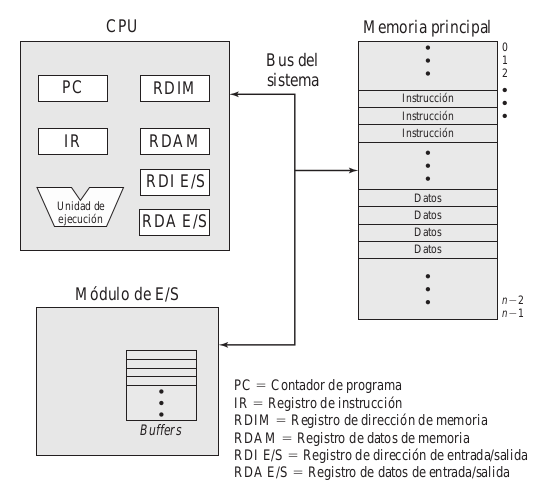
\includegraphics[width=0.8\textwidth, scale=0.5]{figura1.png}
		
			
		\end{figure}
	
		Como se puede apreciar en la figura \ref{fig1.1:componentes} de la págica \pageref{fig1.1:componentes} se muestra un esquema simples de la CPU con sus distintos registros, un esquema de la memoria principal y un esquema de un módulo E/S, y, como se ha dicho antes, todos ellos se comunican a través del bus del sistema. \\
		Una de las funciones del procesador es el itercambio de datos con la memoria. Para este fin, se utilizan normalmente dos registros de internos al procesador: un registro de dirección de memoria (RDIM); que especifica la dirección de memoria de la siguiente lectura o escritura; y un registro de datos de memoria (RDAM), que contiene los datos que se van a escribir en la memoria o que recibe los datos leídos de la memoria. De manera similar, un registro de dirección de E/S (RDIE/S) especifica un determinado dispositivo de E/S, y un registro de datos de E/S (RDAE/S) permite el intercambio de datos entre un módulo de E/S y el procesador. \\ \\
		
		Un módulo de memoria consta de un conjunto de posiciones definidas mediante direcciones numeradas secuencialmente. Cada posición contiene un patrón de bits que se puede interpretar como una instrucción o como datos. Un módulo de E/S transfiere datos desde los dispositivos externos hacia el procesador y la emoria, y viceversa. Contiene buffers (es decir, zonas de almacenamiento internas) que mantienen los datos hasta que se puedan enviar.

	\subsection{Registros del procesador}
		Un proceasdor incluye un conjunto de registros que proporcionan un tipo de memoria que es más rápida y de menor capacidad que la memoria principal. Los registros del procesador sirven para dos funciones:
		
		\begin{itemize}
			\item \textbf{Registros visibles para el usuario.} Permiten al programador en lenguaje máquina o en ensamblador minimizar las referencias a memoria principal optimizando el uso de registros. Para lenguajes de alto nivel, un compilador que realice optimización intentará tomar decisiones inteligentes sobre qué variables se asignan a registros y cuáles a posiciones de memoria principal. Algunos lenguajes de alto nivel, tales como C, permiten al programador sugerir al compilador qué variables deberían almacenarse en registros.
			
			\item \textbf{Registros de control y estado.} Usados por el procesador para controlar su operación y por rutinas privilegiadas del sistema operativo para controlar la ejecución de programas.
		\end{itemize}
		
		No hay una clasificación nítida de los registros entre estas dos categorías. Por ejemplo, en algunas máquinas el contador de programa es visible para el usuario, pero en muchas otras no lo es.
		
		\subsubsection{Registros visibles para el usuario}
		
			A un registro visible para el usuario se puede acceder por medio del lenguaje de máquina ejecutado por el procesador que está generalmente disponible para todos los programas, incluyendo tanto programas de aplicación como programas del sistema. \\ 
			
			El programador puede utlizar los registros de datos para diversas funciones.En algunos casos de propósito general, y pueden usartse con cualquier instrucción máquina que realice operaciones sobre datos. Sin embargo, frecuentemente hay restricciones. Por ejemplo, puede haber registros dedicados a operaciones de coma flotante y otros a operaciones con enteros. \\ 
			
			Los registros de dirección contienen direcciones de memoria principal de datos e instrucciones, o una parte de la dirección que se utiliza en el cálculo de la dirección efectiva o completa. Estos registros puede ser en sí mismos de propósito general, o pueden estar dedicados a una forma, o modo, particular de direccionamiento de memoria. \\
			
			En algunas máquinas, una llamada a una subrutina o a un procedimiento implica salvar automáticamente todos lo registros visibles para el usuario, que se restaurarán al retornar. El \textbf{procesador} realiza estas operaciones de salvar y restaurar como parte de las instrucciones de llamada y retorno. Esto permite que cada procedimiento use estos registros independientemente. En otras máquinas, el programador es el responsable de guardar el contenido de los registros visibles para el usuario antes de una llamada a un procedimiento, inlcuyendo instrucciones para ello en el programa. \textbf{Por tanto las funicones de salvar y restaurar se pueden realizar en hardware o en software, dependiendo del procesador}
			
		\subsubsection{Registros de control y estado}
			
			Se emplean varios registros del procesador para controlar el funcionamiento del mismo. En la mayoría de las máquinas, muchos de ellos no son visibles para el usuario. A algunos de ellos se puede acceder mediante instrucciones máquina ejecutadas en lo que se denomida modo de control o de sistema operativo. \\
			
			Pro supuesto, diferentes máquinas tendrán distintas organizaciones de registros y utilizarán diferente terminología. Los siguientes registros son esenciales para la ejecucion de instrucciones: 
			
			\begin{itemize}
				\item \textbf{Contador de programa (Program Counter,PC)}. Contiene la dirección de la próxima instrucción que se leerá de la memoria
				
				\item \textbf{Registro de instrucción (Instruction Register, IR}. Contiene la última instrucción leída.
			\end{itemize}
				
			\textbf{Todos los diseños de procesador incluyen un registro, o conjunto de registros, conocido como Program Status Word ,PSW, que contiene información de estado}. La PSW contiene normalmente código de condición, además de otra información de estado, tales como un bit para habilitar/inhabilitar las interrupciones y un bit de modo usuario/supervisor.
			
			Los códigos de condición son bits cuyo valor lo asigna normalmente el hardware del procesador teniendo en cuenta el resultado de las operaciones. Los bits de condición se agrupan en uno o más registro. Normalmente, forman parte de un registro de control. Generalmente, las instrucciones de máquina permiten que estos bits se lean mediante una referencia implícita, pero no pueden ser alterador por una referencia explícita debido a que están destinados a la realimentación del resultado de una instrucción. \\
			
			En máquinas que utilizan múltiples tipos de interrupciones, se puede proporcionar un conjunto de registros de interrupciones, con un puntero a cada rutina de tratamiento de interrupción. \\
			
			En el diseño de la organización del registro de control y estado influyen varios factores. Un aspecto fundamental es proporcionar apoyo al sistema operativo. Ciertos tipos de información de control son útiles específicamente para el sistema operativo. Si el diseñador del procesador tiene un conocimiento funcional del sistema operativo que se va a utilizar, se puede diseñar la organización de registros de manera que se proporciones soporte por parte del hardware a característica particulares de ese sistema operativo, en aspectos tales como la protección de memoria y la multiplexación entre programas de usuario. \\
			
			Otra decisión de diseño fundamental es el reparto de la información de control entre los registros y la memoria. Es habitual dedicas las pirmeras cientos o miles de palabras de memoria para propósitos de control. El diseñador debe decidir cuanta información de control debería estar en registros y cuánta en memoria principal. \\
			
			\subsection{Ejecucion de instrucciones}
				Un programa que va a ejecutarse en un procesador consta de un conjunto de instrucciones almacenado en memoria (luego como consecuencia el programa debe estar cargado en memoria principal antes de su ejecución). En su forma más simple, el procesamiento de una instrucción consta de dos pasos: 
				\begin{itemize}
					\item El procesador lee(busca) instrucciones de la memoria, una cada vez.
					\item El procesador ejecuta cada una de las intrucciones que ha leido.
				\end{itemize}
				
				La ejecucion del programa consiste en repetir el proceso de búsqueda y ejecución de instrucciones. La ejecución de la instrucción puede involucrar varias operaciones dependiendo de la naturaleza de la misma. \\
				
				\begin{figure}
				\caption{Figura 2: Ciclo de instrucción básico}
				\label{figura2:instrucción}
				\centering
				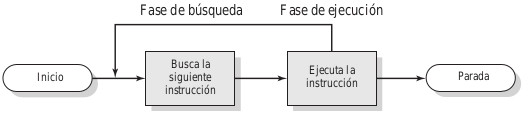
\includegraphics[width=0.8\textwidth, scale=1]{Figura2.png}
				\end{figure}
				
				Se denomina ciclo de instrucción al procesamiento requerido por una única instrucción. En la Figura \ref{figura2:instrucción} de la página \pageref{figura2:instrucción} se describe de forma esquemática las fases del ciclo de instrucción. A estas fases se les denomina fase de búsqueda y fase de ejecución. La ejecución de un programa se detiene sólo si se apaga la máquina, se produce algún tipo de error irrecuperable (excepciones) o se ejecuta una instrucción del programa que para el procesador. \\
				
				\subsubsection{Busqueda y ejecucion de una instruccion}
					Al principio de cada ciclo de instrucción, el procesador lee una instrucción de la memoria. En un procesador típico, el contador del programa (PC) almacena la dirección de la siguiente instrucción que se va a leer. A menos que se le indique otra cosa, el procesador siempre incremente el PC después de cada instrucción ejecutada, de manera que se leerá la siguiente instrucción en orden secuencial. Esta secuencia se puede alterar, por ejemplo, una instrucción del programa podría ser que se actualice el contador de programa a una dirección de memoria concreta si se cumple una determinada condición. \\
					
					La instrucción leída se carga dentro de un registro del procesador conocido como registro de instrucción (IR). La instrucción contiene bits que especifican la acción que debe realizar el procesador. El procesador interpreta la instrucción y lleva a cabo la acción requerida. En general, estas acciones se dividen en cautro categorías:
					
					\begin{itemize}
						\item \textbf{Procesador-memoria}. Se pueden transferir datos desde el procesador a la memoria o viceversa
						\item \textbf{Procesador-E/S}. Se pueden enviar datos a un dispositivo periférico o recibirlos desde el mismo, transfiriéndolo entre el procesador y un módulo de E/S.
						\item \textbf{Procesamiento de datos}. El procesador puede realizar algunas operaciones aritméticas o lógicas sobre los datos.
						\item \textbf{Control}. Una instrucción puede especificar que se va alterar la secuencia de ejecución, como hemos mencionado anteriormente.
					\end{itemize}
					
					Para ver un ejemplo de lo explicado anteriormente se recomienda la página 15 del libro de Sistemas operativos de William Stalling el cual se puede encontrar aqui 
					\href{http://cotana.informatica.edu.bo/downloads/Sistemas%20Operativos.pdf}{SISTEMAS OPERATIVOS: WILLIAM STALLINGS}
					
				
				\subsubsection{Sistema de E/S}
				
				\begin{figure}
					\caption{esquema de ejecución del ejemplo de William Stallings}
					\label{figura3:ejemplo}
					\centering
					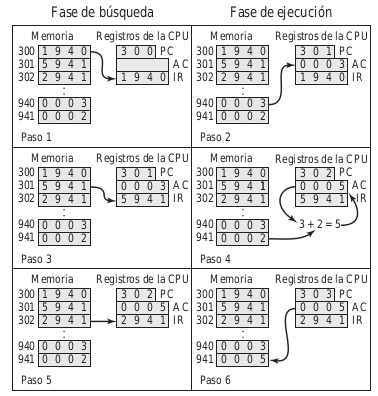
\includegraphics[width=0.8\textwidth, scale=1]{figura3.png}
				\end{figure}
					
					Se pueden intercambiar datos directamente entre un módulo de E/S(ej. un controlador de disco) y el procesador. Al igual que el procesador puede iniciar una lectura o una escritrua en memoria, especificando la dirección de una posición de memoriam, también puede leer o escribir datos en un módulo de E/S. En este caso, el procesador identifica un dispositivo específico que está controlado por un determinado módulo de E/S. Por tanto, podría producirse una secuencia de instrucciones similar a la de la Figura 3 \ref{figura3:ejemplo} en la página \pageref{figura3:ejemplo}, con instrucciones de E/S en vez de instrucciones que hacen referencia a memoria. \\
					
					En algunos casos, es deseable permitir que los intercambios de E/S se produzcan directamente con la memoria para liberar al procesador de la tarea E/S. En tales casos, el procesador concede a un módulo de E/S la autorización para leer o escribir de la memoria, de manera que la transferencia entre memoria y E/S puede llevarse a cabo sin implicar al procesador. Durante dicha transferencia, el módulo de E/S emite mandatos de lectura y escritura a la memoria, liberando al procesador de la responsabilidad del intercambio. esta operación se conoce como acceso directo a memoria (\textit{Direct Memory Access}).
					
			\subsection{Interrupciones}
				Prácticamente todos los computadores proporcionan un mecanismo por el cual otros módulos (memoria y E/S) pueden interrumpir el secuencionamiento normal del procesador. En la tabla \ref{figura4:interrupciones} se incluyen los tipos de interrupciones y sus descripciones.
				
				\begin{figure}
					\centering
					\caption{Clases de interrupciones}
					\label{figura4:interrupciones}
					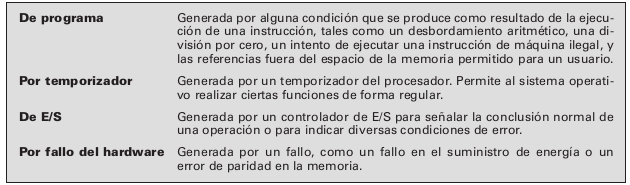
\includegraphics[width=1\textwidth, scale=1]{figura4.png}
				\end{figure}
				
				Básicamente, las interrupciones constituyen una manera de mejorar la utilización del procesador. Por ejemplo, la mayoría de los dispositivos E/S con mucho más lento que el procesador. Supóngase que el procesador está transfiriendo datos a una impresora utilizando el esquema de cilos de instruccions de la Figura \ref{figura2:instrucción}. Después de cada instrucción de escritura, el procesador debe parar y permanecer inactivo hasta que la impresora la lleva a cabo. La longitud de esta puasa puede ser del orden de muchos miles o incluso millones de ciclos de instrucción, luego se desperdicia capacidad del procesador.
				
				\subsubsection{Interrupciones y el ciclo de instrucción}
					Gracias a las interrupciones, el procesador puede dedicarse a ejectuar otras instrucciones mientras que la operación de E/S se está llevando a cabo. Considerese el flujo de control mostrado en \ref{figura5:flujo_programa}(b). Como anteriormente, el programa de usuario alcanza un punto en el que hace una llamada al sistema que consiste en una llamada a ESCRITURA. El programa de E/S que se invoca en este caso consta sólo del código de preparación y el mandato real de E/S. Después de que se ejecuten estas pocas instrucciones, se devuevle el control al programa de usuario. Mientras tanto, el dispositivo externo está ocupado aceptando datos de la memoria del computador e imprimiéndolos. La operación de E/S se lleva a cabo de forma concurrente con la ejecución de instrucciones en el programa de usuario. \\
					
					\begin{figure}
						\caption{Flujo de programa del control sin interrupciones y con ellas}
						\label{figura5:flujo_programa}
						\centering
						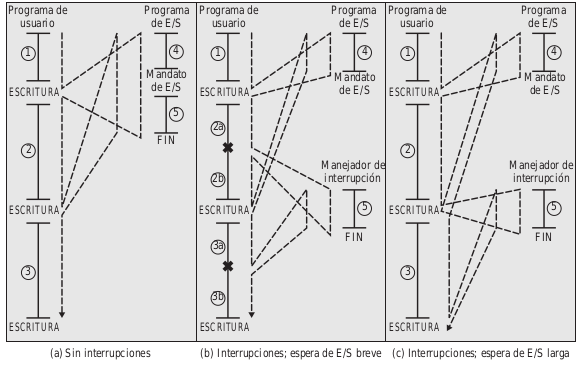
\includegraphics[width=0.8\textwidth, scale=1]{figura5.png}
					\end{figure}

					
					Cuando el dispositivo externo está listo para ser atendido, es decir, cuando está preparado para aceptar más datos del procesador, el módulo de e/S de este dispositivo externo manda una señal de \textit{petición de interrupción} al procesador. El procesador responde suspendiendo la ejecución del programa actual, saltando a la rutina de servicio específica de este dispositivo de E/S, conocida como manejador de interrupción, y reanudando la ejecución original después de haber atendido al dispositivo. \\
					
					De cara al programa de usuario, una interrupción suspende la secuencia normal de ejcución. Cuando se completa el procesamiento de la interrupción, se reanuda la ejecución (Figura \ref{figura6:transferenciacontrol}). Por tanto, el programa de usuario no tiene que contener ningún código especial para tratar las interrupciones; el procesador y el sistema operativo son responsables de suspender el programa de usuario y, posteriormente, reanudarlo en el mismo punto. \\
										
					\begin{figure}
					\caption{Transferencia de control mediante interrupciones}
					\label{figura6:transferenciacontrol}
					\centering
					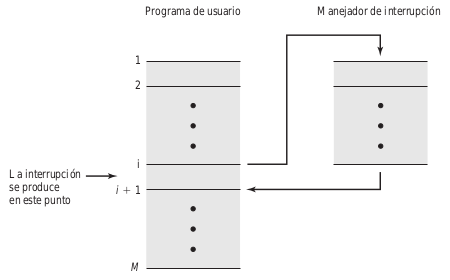
\includegraphics[width=1\textwidth, scale=1]{figura6.png}
					\end{figure}
					
					Para tratar las \textit{interrupciones}, se añade una \textit{fase de interrupción} al ciclo de instrucción, como se muestra en \ref{figura7:instruccionconinterrupcion}. En la fase de interrupción, el procesador comprueba si se ha producido cualquier interrupción, hecho indicado por la presencia de una señal de interrupción. Si no hay interrupciones pendientes, el procesador continúa con la fase de búsqueda y lee la siguiente instrucción del programa actual. Si está pendiente una interrupción, el procesador suspende la ejecución del programa actual y ejecuta la rutina del \textit{manejador de interrupción}. La rutina del manejador de interrupción es generalmente parte del SO. Normalmente, esta rutina determina la naturaleza de la interrupción y realiza las acciones que se requieran. \\
					
					Es evidente que este proceso implica cierta sobrecarga. Deben ejecutarse instrucciones adicionales (en el manejador de interrupción) para determinar la naturaleza de la interrupción y decidir sobre la acción apropiada. Sin embargo, debido a la cantidad relativamente elevada de tiempo que se gastaría simplemente a la espera de una operación de E/S, el procesador se puede emplear mucho más efectivamente con el uso de interrupciones. \\
					
					\begin{figure}
					\caption{Ciclo de instrucción con interrupciones}
					\label{figura7:instruccionconinterrupcion}
					\centering
					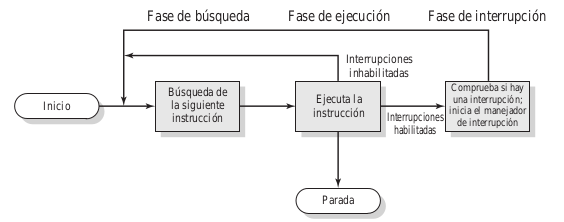
\includegraphics[width=1\textwidth, scale=1]{figura7.png}
					\end{figure}
					
					Comentando el caso de la Figura \ref{figura5:flujo_programa}(c), este caso es un poco especial. Es normal que la operación de E/S tarde mucho más tiempo que la ejecución de una secuencia de instrucciones de usuario, como en este caso. El programa de usuario alcanza la segunda llamada de ESCRITURA ante de que se complete la operación de E/S generada por la primera llamada. El resultado es que el programa de usuario se queda colgado en ese punto. Cuando se ocmpleta la operación de E/S pendiente, se puede procesar la nueva llamada de ESCRITURA y se puede empezar una nueva operación de E/S.
					
					\subsubsection{Procesamiento de interrupciones}
						La aparición de una interrupción dispara varios eventos, tanto en el hardware del procesador como en el software. Cuando un dispositivo de E/S completa una operación de E/S, se produce la siguiente secuencia de evento en el hardware:
						
						\begin{enumerate}
							\item El dispositivo genera una señal de interrupción hacia el procesador.
							\item El procesador termina la ejecución de la instrucción actual antes de responde a la interrupción, como se indica en \ref{figura7:instruccionconinterrupcion}.
							\item El procesador comprueba si hay una petición de interrupción pendiente, determina que hay una y manda una señal de reconocimeinto al dispositivo que produjo la interrupción. Este reconocimiento permite que el dispositivo elimine su señal de interrupción.
							\item En ese momento, el procesador necesita prepararse para transferir el control a la rutina de interrupción. Para comenzar, necesita salvar la información requerida para reanudar el programa actual en el momento de la interrupción. La información mínima requerida es la palabra de estado del programa (PSW) y la posición de la siguiente instrucción que se va a ejecutar, que está contenida en el PC. Esta información se puede apilar en la pila de control de sistema.
							\item A continuación, el procesador cargar el contador del programa con la posición del punto de entra de la rutina de manjeo de interrupción que responderá a esta interrupción. Dependiendo de la arquitectura del computador y del diseño del sistema operativo, puede haber un único programa, uno por cada tipo de interrupción o uno por cada dispositivo y tipo de interrupción. Si hay más de una rutina de manejo de interrupción, el procesador debe determina cuál invocar. Esta información puede estar incluida en la señal de interrupción original o el procesador puede tener que realizar una petición al dispositivo que generó la interrupción para obtener una respuesta que contenga la información requerida. \\ 
							
							Una vez que se ha cargado el contador de programa, el procesador continúa con el siguiente ciclo de instrucción, que comienza con una lectura de instrucción. Dado que la lectura de la instrucción está determinada por el contenido del contador del programa, el resultaod es que se transfiere control al programa manejador de interrupción. La ejecución de este programa conlleva las siguientes operaciones: 
							\item En este momento, el contador del programa y la PSW vinculados con el programa interrumpido se han almacenado en la pila del sistema. Sin embargo, hay otra información que se considera parte del estado del programa en ejecución. En concreto, se necesita salvar el contenido de los registros del procesador, puesto que estos registros los podría utilizar el manejador de interrupciones. Por tanto, se deben salvar todos estos valores, así como cualquier otra información de estado. Generalmente, el manejador de interrupción comenzará salvando el contenido de todos los registros en pila. El puntero de pila se actualiza para que señale a la nueva cima de la pila, mientra que el contador de programa quedará apuntando al principio de la rutina de servicio de interrupción.
							
							\item El manejador de interrupción puede en este momento comenzar a procesar la interrupción. Esto incluirá un examen de la información de estado relacionada con la operación de E/S o con otro evento distinto que haya causado la interrupción. Asimismo, puede implicar el envío de mandatos adicionales o reconocimientos al dispositivo de E/S.
							
							\item Cuando se completa el procesamiento de la interrupción, se recuperan los valores de los registros salvado en la pila y se restituyen en los registros.
							
							\item La última acción consiste en restituir la pila de los valores de la PSW y el contador de programa. Como resultado, la siguiente instrucción que se va a ejecutar corresponderá al programa previamente interrumpido.
							
						\end{enumerate}
						
						
						\begin{figure}
						\caption{Procesamiento simple de interrupciones}
						\label{figura8:procesamientointerrupciones}
						\centering
						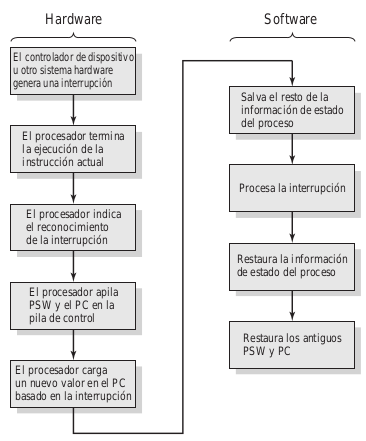
\includegraphics[width=0.8\textwidth, scale=0.8]{figura8.png}
						\end{figure}
						
						Es importante salvar toda la información de estado del programa interrumpido para su posterior reanudación. Esto se debe a que la interrupción no es una rutina llamada desde programa. En su lugar, la interrupción puede suceder en cualquier momento, y, por tanto, en cualquier punto de la ejecución de un programa de usuario. Su aparición es imprevisible. Finalmente, en la Figura \ref{figura8:procesamientointerrupciones} se muestra un esquema de lo explicado en los puntos 1-9.
						
						\subsubsection{Multiples interrupciones}
							Hasta ahora hemos visto solo el caso de que se produzca una única interrupción. Supóngase, sin embargo, que se producen múltiples interrupciones. Por ejemplo, un programa puede estar recibiendo datos de una línea de comunicación e imprimiendo resultados al mismo tiempo. La impresora generará una interrupción cada vez que completa una operación de imprsión. El controlador de la línea de comunicación generará una interrupción cada vez que llega una unidad de datos. La unidad podría consistir en un único carácter o en un bloque, dependiendo de la naturaleza del protocolo de comunicaciones. En cualquier caso, es posible que se produzca una interrupción de comunicación mientras se está procesando una interrupción de la impresora. \\ 
							
							Se pueden considerar dos alternativas a la hora de tratar con múltiples interrupciones. La primera es inhabilitar las interrupciones mientras que se está procesando una interrupción. Una \textit{interrupcion inhabilitada} significa simplemente que el procesador ignorará cualquier nueva señal de petición de interrupción. Si se produce una interrupción durante este tiempo, generalmente permanecerá pendiente de ser procesada, de manera que el procesador sólo la comprobará después de que se rehabiliten las interrupciones. Por tanto, cuando se ejecuta un programa de usuario y se produce una interrupción, se inhabilitan las interrupciones inmediatamente. Después de que se complete la rutina de manejo de interrupción, se rehabilitan las interrupciones antes de reanudar el programa de usuario, y el procesador comprueba si se han producido interrupciones adicionales. Es una estrategia válida y sencilla puesto que las interrupciones se manejan en estricto orden secuencial (Véase \ref{figura9:secuencial}). \\
							
							\begin{figure}
							\caption{Procesamiento secuencial de interrupciones}
							\label{figura9:secuencial}
							\centering
							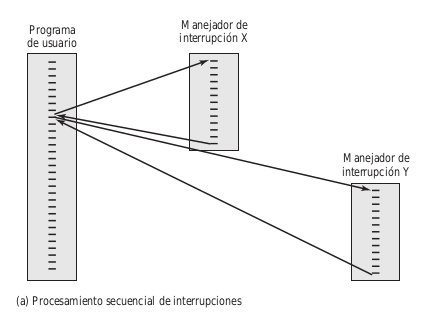
\includegraphics[width=1\textwidth, scale=1]{figura9.png}
							\end{figure}
							
							La desventaja de la estrategia anterior es que no tiene en cuenta la prioridad relativa o el grado de urgencia de las interrupciones. Por ejemplo, cuando llegan datos por la línea de comunicación puede necesitar que se procesen rápidamente de manera que se deje sitio para otros datos que puedan llegar. Si el primer lote de datos no se ha procesado antes de que llegue el segudno, los datos pueden perderse porque le \textit{buffer} del dispositivo de E/S pueden llenarse y desbordarse. \\
							
							Una segunda estrategia es definir prioridades para las interrupciones y permitir que una interrupción de más prioridad cause que se interrumpa la ejecución de un manejador de una interrupción de menor prioridad(\ref{figura10:anidado}). Finalmente definiremos un concepto \textbf{ISR}(\textit{Interrupt Service Routine}).
							
							\begin{figure}
							\caption{Procesamiento anidado de interrupciones}
							\label{figura10:anidado}
							\centering
							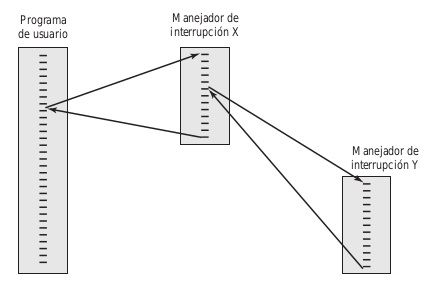
\includegraphics[width=0.8\textwidth, scale=1]{figura10.png}
							\end{figure}
							
						
						\subsubsection{Multiprogramación}
							Incluso utilizando interrupciones, puede que el procesador siga sin utilizarse eficientemente. Si el tiempo requerido para completar una operación de E/S es mucho mayor que el código de usuario entre las llamadas de E/S, el procesador estará parado la mayor parte del tiempo. Ua solución a este problema es permitir que múltiples programas de usuario estén activos al mismo tiempo. \\
							
							Supóngase, por ejemplo, que el procesador tiene que ejecutar dos programas. Uno de ellos simplemente se dedica a leer datos de la memoria y copiarlos a un dispositivo externo; el otro el algún tipo de aplicación que implica mucho cálculo. El procesador puede empezar con el programa que genera salida, emitir un mandato de escritura y, a continuación, empezar la ejecución de la otra aplicación. Cuando el procesador trata con varios programas, la secuencia en la que se ejecutan los programas dependerá de su prioridad relativa, así como de si están esperando la finalización de una operación de E/S. Cuando se interrumpe un programa y se transfiere el control a un manejador de interrupción, una vez que se ha comletado la rutina del manejador de interrupción, puede ocurrir que no se le devuelva inmediatamente el control al programa de usuario que estaba en ejecución en ese momento. En su lugar, el control puede pasar a algún otro programa pendiente de ejecutar que tenga una prioridad mayor. Posteriormente, se reanudará el programa de usuario interrumpido previamente, en el momento en que tenga la mayor prioridad. Este concepto de múltiples programas que se ejecutan en turno se denomina multiprogramación.
							
					\subsection{Técnicas de comunicación E/S}
						\subsubsection{E/S programada}
							Cuando el procesador ejecuta un programa y encuentra una instrucción relacionada con la E/S, ejecuta esa instrucción generando un mandato al módulo de E/S apropiado. En el caso de la E/S programada, el módulo de E/S realiza la acción solicitada y fija los bits correspondientes en el registro de estado de E/S, pero no realiza ninguna acción para avisar al procesador. En concreto, no interrumpe al procesador. Por tanto, después de que se invoca la instrucción de E/S, el procesador debe tomar un papel actio para determinar cuándo se completa la instrucción de E/S. Por este motivo, el procesador comprueba periódicamente el estado del módulo de E/S hasta que encuentra que se ha completado la ejecución.  \\ 
							
							Con esta técnica, el procesador es responsable de extraer los datos de la memroia principal en una operación de salida y de almacenarlo en ella en una operación de entrada. El software de E/S se escribe de manera que el procesador ejecuta instrucciones que le dan control directo de la operación de E/S, incluyendo comprobar el estado del dispositivo, enviar un mandato de lectura o de escritura, y transferir los datos. Por tanto, el juego de instrucciones incluye instrucciones de E/S de las siguientes categorías:
							
							\begin{itemize}
							\item \textbf{Control.} Utilizadas para activar un dispositivo externo y especificarle qué debe hacer. Por ejemplo, se le puede indicar a una unidad de cinta magnética que se rebobine o avance un registro.
							\item \textbf{Estado.} Utilizadas para comprobar diversas condiciones de estado asociadas a un módulo de E/S y sus periféricos.
							\item \textbf{Transferencia.} Utilizadas para leer y/o escribir datos entre los registros del procesador y los dispositivos externos.
							\end{itemize}
							
							\begin{figure}
							\caption{Tres técnicas para leer un bloque de datos}
							\label{figura11:tecnicasE/S}
							\centering
							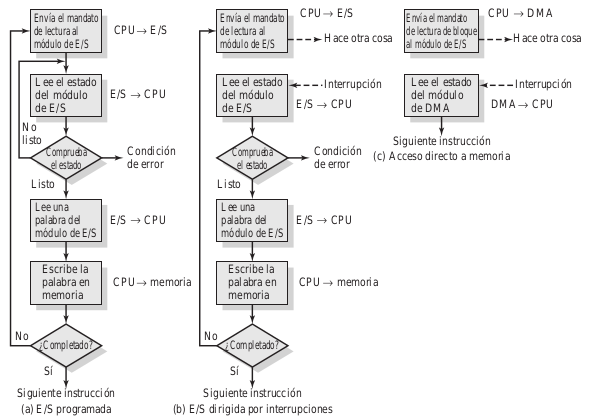
\includegraphics[width=1\textwidth, scale=1]{figura11.png}
							\end{figure}
							
						\subsubsection{E/S dirigida por interrupciones}
							El problema de la E/S programada es que el procesador tiene que esperar mucho tiempo hasta que el módulo E/S correspondiente esté listo para la recepción o la transmisión de más datos. El procesador, mientras está esperando, debe comprobar repetidamente el estado del módulo de E/S. Como resultado, el nivel de rendimiento de todo el sistema se degrada gravemente. \\
							
							Una alternativa es que el procesador genera un mandato de E/S para un módulo y, acto seguido, continúa realizando algún otro trabajo útil. El módulo de E/S interrumpirá más tarde al procesador para solicitar su servicio cuando esté listo para intercambiar datos con el mismo. El procesador ejecutará la transferencia de datos, como antes, y después reanudará el procesamiento previo. \\
							
							Para una operación de entrada, el módulo de E/S recibe un mandato de LECTURA del procesador. El módulo de E/S pasa entonces a leer los datos de un periférico asocidado. Una vez que los datos están en el registro de datos del módulo, este genera una interrupción al procesador a través de una línea de control. El módulo entonces espera hasta que el procesador pida sus datos. Cuando se hace la petición, el módulo sitúa sus datos en el bus de datos y ya está listo para otra operación de E/S. \\
							
							Desde el punto de vista del procesador, las acciones correspondientes a una operación de lectura son las que se describen a continuación. El procesador genera un mandato de LECTURA. Salva en la pila del sistema el contexto del programa actual (PSW, PC y registros) y lo abandona, pasando a hacer otra cosa. Al final de cada ciclo de instrucción el procesador comprueba si hay interrupciones. Cuando se produce la interrupción del módulo de E/S, el procesador salva el contexto del programa que se está ejecutando actualmente y comienza a ejecutar un programa de manejo de interrupción que procesa la interrupción. En este caso, el procesador lee la palabra de datos del módulo de E/S y la almacena en meoria. A continuación, restaura el contexto del programa que había realizado el mandato de E/S (o de algún programa) y reanuda su ejecución. \\
							
							Casi invariablemente, habrá múltiples módulos de E/S en un computador, por lo que se necesitan mecanismos para permitir que el procesador determina qué dispositivo causó la interrupción y decidir, en caso de múltiples interrupciones, cúal debe manejar primero. En algunos sistemas, hay múltiples líneas de interrupción, de manera que cada módulo de E/S usa una línea diferente. Cada línea tendrá una prioridad diferente. Alternativamente, puede haber una única línea de interrupción pero se utilizan líneas adicionales para guardar la dirección de un dispositivo. De nuevo, se le asignan diferentes prioridades a los distintos dispositivos.
							
						
						\subsubsection{Acceso directo a memoria}
							La E/S dirigida por interrupciones, aunque más eficiente que la E/S programada simple, todavía requiere la intervención activa del procesador para transferir datos entre la memoria y un módulo de E/S, ya que cualquier transferencia de datos debe atravesar un camino a través del procesador. Por tanto, ambas formas de E/S sufren dos inconvenientes inhernetes:
							
							\begin{itemize}
								\item La tasa de transferencia de E/S está limitada por la velocidad con la que el procesador puede comprobar el estado de un dispositivo y ofrecerle servicio.
								\item El procesador está involucrado en la gestión de una transferencia de E/S; se deben ejecutar varias instrucciones por cada transferencia de E/S.
							\end{itemize}
							
							Cuando se van a transferir grande volúmenes de datos, se requiere una técnica más eficiente: el acceso directo a memoria (\textit{Direct Memory Access}, DMA). La función de DMA puede llevarla a cabo un módulo separado conectado en el bus del sistema o puede estar incluida en un módulo de E/S. En cualquier caso, la técnica funciona como se describe a continuación. Cuando el procesador desea leer o escribir un bloque de datos, genera un mandato al módulo de DMA, enviándole la siguiente información:
							
							\begin{itemize}
								\item Si se trata de una lectura o de una escritura.
								\item La dirección del dispositivo de E/S involucrado.
								\item La posición inicial de memoria en la que se desea leer los datos o donde se quieren escribir.
								\item El númereo de palabras que se pretende leer o escribir
							\end{itemize}
							
							A continuación, el procesador continúa con otro trabajo. El módulo de DMA transferirá el bloque completo de datos, palabra a palabra, hacia la memoria o desde ella sin pasar a través del procesador. Por tanto, el procesador solamente está involucrado al principio y al final de la transferencia. \\
							
							El módulo de DMA necesita tomar el control del bus para transferir datos hacia la memoria o desde ella. Debido a esta competencia en el uso del bus, puede haber veces en las que el procesador necesita el bus y debe esperar al módulo de DMA. Nótese que esto no es una interrupción; el procesador no salva un contexto y pasa a hacer otra cosa. En su lugar, el procesadro se detiene durante un ciclo de bus ( el tiempo que se tarda en transferir una palabra a través del bus). El efecto global es causar que el procesador ejecute más lentamente durante una transfernecia de DMA en el caso de que el procesador requiera acceso al bus. Sin embargo, para una transferencia de E/S de múltiples palabras, el DMA es mucho más eficiente que la E/S dirigida por interrupciones o programada.
							
		
					\subsection{Control de procedimientos} \label{Control de procedimientos}
						Una técnica habitual para controlar la ejecución de llamadas a procedimiento y los retornos de los mismos es utilizar una pila. 
						
						\subsubsection{Implementación de la pila}
							Una pila es un conjunto ordenado de elementos, tal que en cada momentos solamente se puede acceder a uno de ellos (el más recientemente añadido). El pnto de acceso se denomina \textbf{cima} de la pila. El numero de elementos de la pila, o longitud de la pila, es variable. Poresta razón, se conoce también una pila como una lista de aplimiento o lista donde el último que entra es el primero que sale (\textit{Last In First-Out}, FIFO). \\
							
							La implementación de una pila requiere que haya un conjunto de posiciones dedicado a almacenar los elementos de la pila. Se reserva en memoria principal (o memoria virtual) un bloque contiguo de posiciones. La mayoría de las veces el bloque está parcialmente lleno con elementos de la pila y el resto está disponible para el crecimiento de la pila. Se necesitan tres direcciones para un funcionamiento adecuado, que habitualmente se almacenan en registros del procesador:
							
							\begin{itemize}
								\item \textbf{Puntero de pila.} Contiene la dirección de la cima de la pila. Si se añade un elemento(APILA) o se elimina (EXTRAE), el puntero se decrementa o incrementa para contener la dirección de la nueva cima de la pila.
								\item \textbf{Base de la pila.} Contiene la dirección de la posición inferior en el bloque reservado. Se trata de la primera posición que se utiliza cuando se añada un elemento a una pila vacía. Si se hace un intento de extraer un elemento cuando la pila está vacía, se informa del error.
								\item \textbf{Límite de la pila.} Contiene la dirección del otro extremo del bloque reservado. Si se hace un intento para apilar cuando la pila esta llena, se indica un error.
								
							\end{itemize}
							
							Tradicionalmente, y en la mayoría de las máquinas actuales, la base de la pila está en el extremo con la dirección más alta del bloque de pila reservado, y el límite está en el extremo con la dirección más baja.
							
							\begin{figure}
							\caption{Organización habitual de la pila}
							\label{figura12:pila}
							\centering
							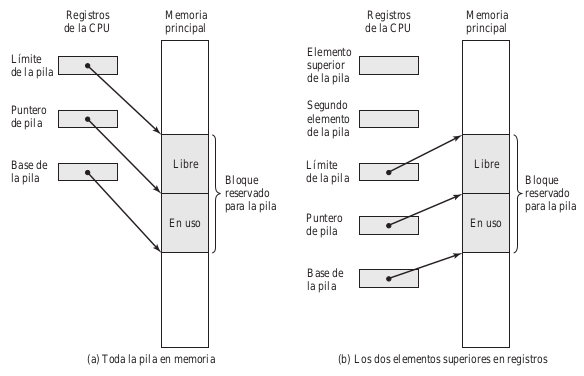
\includegraphics[width=1\textwidth, scale=1]{figura12.png}
							\end{figure}
							
						\subsubsection{Llamadas y retornos de procedimientos}
							Una técnica habitual para gestionar las llamadas y los retornos de los procedimientos es utilizar una pila. CUando el procesador ejectua una llamada, se almacena (apila) la dirección de retorno en la pila. Cuando se ejecuta un retorno, se utiliza la dirección de la cima de la pila y se elimina (extrae) esa dirección de la pila. \\
							
							Es también necesario con frecuencia pasar parámetros en una llamada a procedimiento. Estos se podrían pasar en los registros. Otra posibilidad es almacenar los parámetros en la memoria justo después de las instrucciones de llamada. En este caso, el retorno debe estar en la posición siguiente a los parámetros. Ambas técnicas tienen sus inconvenientes. Si se utilizan los registros, el programa llamado y el que realiza la llamada deben escribirse de maner que se asegure que los registros se utilizan apropiadamente. El almacenamiento de parámetros en memoria hace difícil intercambiar un número variable de parámetros. \\
							
							Una estrategia más flexible para el paso de parámetros es la pila. Cuando el procesador ejecuta una llamada, no sólo apila la direcciónde retorno, sino también los parámetros que se desean pasar al procedimiento llamado. El procedimiento invocado puede acceder a los parámetros en la pila. Al retornar, los parámetros de retorno se pueden almacenar también en la pila, debajo de la dirección de retorno. El conjunto completo de parámetros, incluyendo la dirección de retorno, que se almacena en una invocación de un procedimiento se denomina marco de pila. \\
							
							\begin{figure}
							\caption{Crecimiento del marco de pila utilizando los procesos de ejemplo P y Q}
							\label{figura13:ejemplopil}
							\centering
							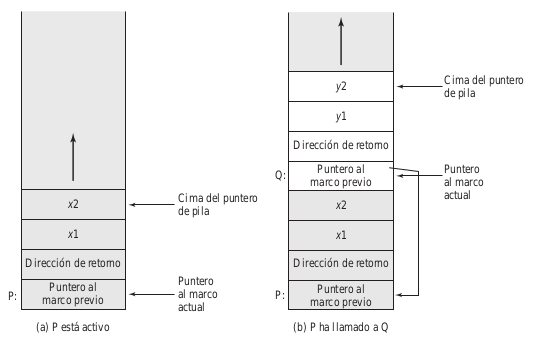
\includegraphics[width=0.8\textwidth, scale=1]{figura13.png}
							\end{figure}
							
							En la Figura \ref{figura13:ejemplopil} se muestra un ejemplo. Este se refiere a un procedimiento P en el que se declaran las variables locales $x_1$ y $x_2$, y el procedimiento Q, al cual puede llamar P y en el que se declaran las variables $y_1$ y $y_2$. El primer elemento almacenada en cada marco de pila es un puntero al marco de pila previo. Esta técnica se necesita si el número o la longitud de los parámetros que se van a apilar es variable. A continuación, se almacena el punto de retorno del procedimiento que corresponde a este marco de pila. Finalmete, se reserva espacio en la cima del marco de pila para las variables locales. Estas variables locales se pueden utilizar para el paso de parámetros. Por ejemplo, supóngase que cuando P llama a Q le pasa un valor como parámetro. Este valor se podría almacenar en la variable $y_1$. \\
							
							Cuando se ejecuta esta llamada, se crea un nuevo marco de pila para Q (Figura \ref{figura13:ejemplopil}(b)), que incluye un puentero al marco de pila para P, la dirección de retorno de P, y dos variables locales para Q, una de las caules se inia con el valor pasado como parámeto desde P. La otra variable local, $y_2$, es simplemente una variable local utilizada por Q en sus cálculos.
							
						\subsubsection{Procedimientos reentrantes}
							Un concepto útil, particularmente en un sistema que da soporte a múltiples usuarios al mismo tiempo, es el de los procedimientos reentrantes. Un procedimiento reentrante es aquel en el que una única copia del código del programa se puede compartir por múltiples usuarios durante el mismo periodo de tiempo. El carácter reentrante de un procedimiento tiene dos aspectos fundamentales: el código del programa no puede modificarse a sí mismo y los datos locales de cada usuario deben almacenarse separadamente. Un procedimiento reentrante puede ser interrumpido e invocado por el programa que causó la interrupción y, a pesar de ello, ejecutarse correctamente al retornar al procedimiento. En un sistema compartido, el carácter reentrante permite un  uso más eficiente de la memoria principal. Se mantiene una copia del código del programa en memoria principal, pero más de una aplicación puede llamar al procedimiento. \\
							
							Por tanto, un procedimiento reentrante debe tener una parte permanente (las instrucciones que constituyen el procedimiento) y una parte temporal (un puntero de retorno al programa que realizó la llamada, así como espacio para las variables locales usadas por el programa). Cada instancia de la ejecución, llamada de activación, de un procedimiento ejecutará el código en la parte permanente pero debe tener su propia copia de los parámetros y las variables locales. La parte temporal asociada con una activación en particular se denomina registro de activación. \\
							
							La manera más conveniente de dar soporte a los procedimientos reentrantes es mediante una pila. Cuando se llama a un procedimiento reentrante, el registro de activación del procedimiento se puede almacenar en la pila. Por tanto, el registro de activación se convierte en parte del marco de pila que se crea en la llamada a procedimiento. \\
					
				
				\section{Estructura del sistema operativo}	
					\subsection{Objetivos y funciones de los SOs}
						\subsubsection{El sistema operativo como una interfaz de usuario/computador}
						El hardware y software utilizados para proporcionar aplicaciones a los usuarios se pueden ver de forma jerárquica o en capas, tal y como	se ve en la figura \ref{figura14:capasScomputacion}. El usuario de dichas aplicaciones es decir, el usuario final, normalmente no se preocupa por los detalles del hardware del computador. Por tanto, el usuario final ve un sistema de computación en términos de un conjunto de aplicaciones. Una aplicación se puede expresar en un lenguaje de programación. Si un programador tuviera que desarrollar una aplicación como un conjunto de instrucciones de código máquina que se encargaran de controlar completamente el hardware del computador, se enfrentaría a una labor extremadamente compleja. Para facilitar esta labor, se proporcionan un conjunto de programas del sistema (algunos se denominan utilidades). Estos utilizan frecuentemente funciones que asisten al programador en las fases de creación de programas, gestión de ficheros y control de dispositivos de E/S. Un programador hará uso de estas utilidades cuando desarrolle una aplicación, y las aplicaciones, invocarán a las utilidades durante su ejecución. El SO es el porgrama de sistema más importante. Este oculta los detalles del hardware al programador y le proporciona una interfaz apropiada para utilizar el sistema. Actúa como mediador, haciendo más fácil al programador y a la aplicación el acceso y uso de dichas utilidades y servicios.
						
							\begin{figure}
							\caption{Capas y vsitas de un sistema de computación}
							\label{figura14:capasScomputacion}
							\centering
							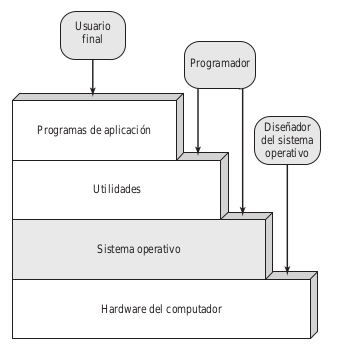
\includegraphics[width=0.8\textwidth, scale=1]{figura14.png}
							\end{figure}
					
					De froma resumida el SO proporciona servicio en:
					\begin{itemize}
					\item \textbf{Desarrollo de programas.} El SO proporciona una variedad de utilidades y servicios para asistir al programador en la creación de los programas. Normalmente, estos servicios se ofrecen en la forma de utilidades que, aunque no forman parte del núcleo del SO, se ofrecen con dicho sistema y se conocen como herramientas de desarrollo de programas de aplicación.
				
					\item \textbf{Ejecución de programas.} Se necesita realizar una serie de pasos para ejecutar un programa. Las instrucciones y los datos se deben cargar en memoria principal. Los dispositivos de E/S y los ficheros se deben inicializar, y otros recursos deben prepararse. Los sistemas operativos realizan estas labores de planificación en nombre del usuario
				
					\item \textbf{Acceso a dispositivos de E/S.} Cada dispositivo de E/S requiere su propio conjunto peculiar de instrucciones o señales de control para cada operación. El sistema operativo proporciona una interfaz uniforme que esconde esos detalles de forma que los programadores puedan acceder a dichso dispositivos utilizando lecturas y escrituras sencillas.
				
					\item \textbf{Acceso controlado a ficheros.} Para el acceso a los ficheros, el sistema operativo debe reflejar una comprensión detallada no sólo de la naturaleza del dispositivo de E/S, sino también de las estructura de los datos contenidos en los ficheros del sistema de almacenamiento. Adicionalmente, en el caso de un sistema con múltiples usuarios, el sistema operativo puede proporcionar mecanismos de protección para controlar el acceso a los ficheros.
				
					\item \textbf{Acceso al sistema.} Para sistemas compartidos o públicos, el sistema operativo controla el acceso al sistema completo y a recursos del sistema específicos. La función de acceso debe proporcionar protección a los recursos y a los datos, evitando el uso no autorizado de los usuarios y resolviendo conflictos en el caso de conflicto de recursos.
				
					\item \textbf{Detección y respuesta de errores.} Se pueden dar gran variedad de errorres durante la ejecución de un sistema de computación. Estos incluyen errores de hardware internos y externos (ej. erro de memoria, fallo de dispositivo), y diferentes errores software (división por cero, acceso a memoria prohibida \ldots). En cada caso, el sistema operativo debe proporcionar una respuesta que elimine la condición de error, suponiendo el menor impacto en las aplicaciones que están en ejecución. La respuesta puede oscilar entre finalizar el programa que causó el error hasta reintentar la operación o simplemente informar del error a la aplicación.
				
					\item \textbf{Contabilidad.} Un buen SO recogerá estadísticas de uso de los diferentes recursos y monitorizará parámetros de rendimiento tales como el tiempo de respuesta. En cualquier sistema, esta información es útil para anticipar las necesidades de mejoras futuras y para opotimizar el sistema a fin de mejorar su rendimiento. En un sistema multiusuario, esta información se puede utilizar para facturar a los diferentes usuarios.
				
					\end{itemize}
		
				\subsubsection{El SO como gestor de recursos}							
					Un computador es un conjunto de recursoso que se utilizan para el transporte, almacenamiento y procesamiento de los datos, así como para llevar a cabo el control de estas funciones. El SO se encarga de gestionar estos recursos \\
					
					El sistema operativo es un mecanismo de control inusual en dos aspectos:
						\begin{itemize}
						\item Las funciones del SO actúan de la misma forma que el resto del software; es decir, se trata de un programa o conjunto de programas ejecutados por el procesador.
						
						\item El sistema operativo frecuentemente cede el control y depende del procesador para volver a retomarlo.
						
						\end{itemize}		
						
					
					El SO es un conjunto de programas, que proporcionan instrucciones para el procesador. La principal diferencia respecto a un programa cualquiera radica en el objetivo del mismo. El SO dirige al procesador en el uso de los otros recursos del sistema y en la temporarización de la ejecución de otros programas. No obstante, para que el procesador pueda realizar esto, el sistema operativo debe dejar paso a la ejecución de otros programas. Luego, el SO deja el control para que el procesador pueda realizar trabajo útil y de nuevo retoma el control para permitir al procesador que realice la siguiente pieza del trabajo. \\
					
					Una porción del SO se encuentra en la memoria principal. Esto incluye el \textbf{kernel}, o \textbf{núcleo}, que contiene las funciones del sistema operativo más frecuentemente utilizadas y, en cierto momento, otras porciones del SO actualmente en uso. El resto de la memoria principal contiene programas y datos de usuario. La asignación de este recurso es controlada de forma conjunto por el SO y el hardware de gestión de memoria para el procesador.	El SO decide cuándo un programa en ejecución puede utilizar un dispositivo de E/S y controla el acceso y el uso de los ficheros. El procesador es también un recurso, y el sistema operativo debe determinar cuánto tiempo de procesador debe asignarse a la ejecución de un programa de usuario particular. En el caso de un sistema multiprocesador, esta decisión debe ser tomado por todos los procesadores. \\
										
					\begin{figure}
					\caption{El SO como gestor de recursos}
					\label{figura15:gestor_recursos}
					\centering
					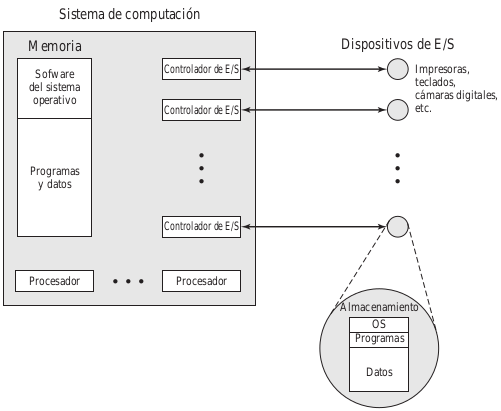
\includegraphics[width=0.8\textwidth, scale=1]{figura15.png}
					\end{figure}
					
				\subsubsection{Facilidad de evolución de un sistema operativo}
					Un sistema operativo importante debe evolucionar en el tiempo por las siguiente razones:
						
						\begin{itemize}
						\item \textbf{Actualizaciones de hardware más nuevos tipos de hardware.}
						\item \textbf{Nuevos servicios.} En respuesta a la demanda del usuario o en respuesta a las necesidades de los gestores de sistema, el sistema operativo debe ofrecer nuevos servicios.
						\item \textbf{Resolución de fallos.} Cualquier sistema operativo tiene fallos. Estos fallos se descubren con el transcurso del tiempo y se resueven. Por suspuesto, esto implica la introducción de nuevos fallos.
						\end{itemize}
						
					La necesidad de cambiar regularmente un sistema operativo introduce ciertos requisitos en su diseño. Un hecho obvio es que el sistema debe tener un diseño modular, con interfaces entre los módulos claramente definidas, y que debe estar bien documentado. Para programas grandes, tal como el típico sistema operativo contemporáneo, llevar a cabo una modularización sencilla no es adecuado.
					
			\subsection{La evolución de los sistemas operativos}
				\subsubsection{Procesamiento serie}
					Con los primeros, computadores, desde finales de los años 40 hasta mediados de los años 50, el programador interaccionaba directamente con el hardware del computador; no existía ningún sistema operativo. Estas máquinas eran utilizadas desde una consola que contenía luces, interruptores, algún dispositivo de entrada y una impresora. Los programas en código máquina se cargaban a través del dispositivo de entrada. Si un error provocaba la parada del programa, las luces indicaban la condición del error. El programador podía entonces examinar los registros del procesador y la memoria principal para determinar la causa del error. Si el programa terminaba de forma normal, la salida aparecía en la impresora.
				
				Estos sistemas presentaban dos problemas principales:
					\begin{itemize}
					\item \textbf{Planificación.} La mayoría de las instalaciones utilizaban una plantilla impresa para reservar tiempo de máquina. Típicamente, un usuario podía solicitar un bloque de tiempo en múltiplos de media hora aproximadamente. Un usuario podía obtener una hora y terminar en 45 minutos; esto impilicaba malgastar tiempo de procesamiento del computador. Por otro lado, el usuario podía tener problemas, si no finalizaba en el tiempo asignado y era forzado a terminar entes de resolver el problema.
					\item \textbf{Tiempo de configuración.} Un único programa (\textbf{trabajo}) podía implicar la carga en memoria del compiladory del programa en lenguaje de alto nivel y a continuación la carga y el enlace del programa objeto y las funciones comunes. Cada uno de estos pasos podía suponer montar y desontar cintas o configurar tarjetas. Si ocurría un error, el desgraciado usuario normalmente tenía que volver al comienzo de la secuencia de configuración. Luego se utilizaba mucho tiempo en configurar el programa a ejecutar.
					\end{itemize}
					
					Este modo de operación puede denominarse procesamiento en serie, para reflejar el hecho de que los usuario acceden al computador en serie. A lo largo del tiempo se han desarrollado varias herramientas de software de sistemas con el fin de realizar el procesamiento en serie más eficientes (bibliotecas comunes, enlazadores, cargadores, depuradores, y rutinas de gestión de E/S \ldots).
					
				\subsubsection{Sistemas en lotes sencillos}
					Las primeras máquinas eran muy caras, y por tanto, era importante maximizar su utilización. El tiempo malgastado en la planificación y configuración de los trabajos era inaceptable. 
					
					Para mejorar su utilización, se desarrolló el concepto de sistema operativo por lotes. La idea central bajo el esquema de procesamineto en lotes sencillo es el uso de una pieza de software denominada \textbf{monitor}. Con este tipo de SO, el usuario no tiene que acceder directamente a la máquina. En su lugar, el usuario envía un trabajo a través de una tarjeta o cinta al operador del computador, que crea un sistema por lotes con todos los trabajos enviados y coloca la secuencia de trabajos en el dispositivo de entrada, para que lo utilice el monitor. Cuando un programa finaliza su procesamiento, deuvelve el control al monitor, punto en el cual dicho monitor comienza la carga del siguiente programa.
					
					\begin{itemize}
					\item \textbf{Punto de vista del monitor.} El monitor controla la secuencia de eventos. Para ello, una gran parte del monitor debe estar en memoria principal y disponible para la ejecución. Esta porción es el \textbf{monitor residente}. El resto del monitor está formado por un conjunto de utilidades y funciones comunes que se cargan como subrutinas en el programa de usuario, al comienzo de cualquier trabajo que las requiera. El monitor lee de uno en uno los trabajos desde el dispositivo de entrada. Una vez leído el dispositivo, el trabajo actual se coloca en el área de programa de usuario, y se le pasa el control. Cuando el trabajo se ha completado, devuelve el control al monitor, que inmediatamente lee el siguienete trabajo. Los resultados de cada trabajo se envían a un dispositivo de salida.
					
					\item \textbf{Punto de vista del procesador.} En un cierto punto, el procesador ejecuta instrucciones de la zona de memoria principal que contiene al monitor. Estas instrucciones provocan que se lea el siguiente trabajo y se almacene en otra zona de memoria principal. Una vez que el trabajo se ha leído, el procesador encontrará una instrucción de salto en el monitor que le indica al procesador que continúe la ejecución al inicio del programa de usuario. El procesador entonces ejecutará las instrucciones del programa de usuario hasta que encuentre una condición de finalización o error. Cualquiera de esta condiciones hace que el procesador ejecute la siguiente instrucción del programa monitor. 
					\end{itemize}
					
					En la figura \ref{figura16:sistemaenlotes} se puede observar un esquema de la disposición de memoria.
										
					\begin{figure}
					\caption{Disposición de memoria de un monitor residente}
					\label{figura16:sistemaenlotes}
					\centering
					\includegraphics[width=0.4\textwidth, scale=0.5]{figura16.png}
					\end{figure}
					
					El monitor realiza una función de planificación: en una cola se sitúa un lote de trabajos, y los trabajos se ejecutan lo más rápidamente posible, sin ninguna clase de tiempo ocioso entre medias. Además, el monitor mejora el tiempo de configuración de los trabajos. Con cada uno de los trabajos, se incluye un conjunto de instrucciones en algún formato primitivo de \textbf{lenguaje de control de trabajos} (\textit{Job Control Language}, JCL). Se trata de un tipo especial de lenguaje de programación utilizado para dotar de instrucciones al monitor.m\\
					
					Durante la ejecución del programa de usuario, cualquier instrucción de entrada implica la lectura de una línea de datos. La instrucción de entrada del programa de usuario supones la invocación de una rutina de entrada, que forma parte del SO. La rutina de entrada comprueba que el programa no lea accidentalmente una línea JCL. Si esto sucede, se genera un error y se transfiere el control al monitor. Al finalizar el trabajo de usuario, el monitor analizará todas las líneas de entrada hasta que encuentra la siguiente instrucción JCL. De esta forma, el sistema queda protegido frente un programa con excesivas o escasas líneas de datos. \\
					
					El monitor, o SO en lotes, es simplemente un programa. Este confía en la habilidad del procesador para cargar instrucciones de diferentes porciones de la memoria principal que de forma alternativa le permiten tomar y abandonar el control. Otras características hardware deseables son:
					
					\begin{itemize}
					\item \textbf{Protección de memoria.} Durante la ejecución del programa de usuario, éste no debe alterar el área de memoria que contiene al monitor. Si esto ocurriera, el hardware del procesador debe detectar un error y transferir el control al monitor. El monitor entonces abortará el trabajo, imprimirá un mensaje de error y cargará el siguiente trabajo.
					
					\item \textbf{Temporizador.} Se utiliza un temporizador para evitar que un único trabajo monopolice el sistema. Se activa el temporizador al comienzo de cada trabajo. Si el temporizador expira, se para el programa de usuario, y se devuelve el control al monitor.
					
					\item \textbf{Instrucciones privilegiadas.} Ciertas instrucciones a nivel de máquina se denominan privilegiadas y sólo las puede ejecutar el monitor. Si el procesador encuentra estas instrucciones mientras ejecuta un programa de usuario, se produce un error provocando que el control se transfiera al monitor. Entre las instrucciones privilegiadas se encuentran las instrucciones de E/S, que permiten que el monitor tome control de los dispositivos de E/S. Esto evita, por ejemplo, que un programa de usuario de forma accidental lea instrucciones de control de trabajos del siguiente trabajo. Para realizar operaciones de E/S el prgorama debe solicitar al monitor que las realice.
					
					\item \textbf{Interrupciones.} Los modelos de computadores iniciales no tenían esta capacidad. Esta característica proporciona al sistema operativo más flexibilidad para dejar y retomar el control desde los programa de usuario.
					\end{itemize}
							
					Un programa de usuario ejecuta en modo usuario, en el cual los usuarios no peuden acceder a ciertas áreas de memoria y no pueden ejecutar ciertas instrucciones. El monito ejecuta en modo sistema, o lo que se denomina modo núcleo, en el cual se pueden ejecutar instrucciones privilegiadas y se puede acceder a áreas de memoria protegidas. \\
					
					No es recomendable construir un SO sin estas características, aunque se puede. Con un SO en lotes, el tiempo de máquina alterna la ejecución de programas de usuario y la ejecución del monitor. Esto implica dos sacrificios: el monitor utiliza parte de la memoria principal y consume parte del tiempo máquina. Ambas situaciones implican una sobrecarga. A pesar de esta sobrecarga, el sistema en lotes mejora la utilización del computador.	\\
					
				
				\subsubsection{Sistemas en lotes multiprogramados}
					El procesador se encuentra frecuentementes ocios, incluso con el secuenciamiento de trabajos automático que proporciona un sistema operativo en lotes simple. El problema consiste en que los dispositivos de E/S son lentos comparados con el procesador. El procesador ejecuta durante cierto tiempo hasta que alcanza una instrucción de E/S. Entonces debe esperar que la instrucción de E/S concluya antes de continuar. \\
					
					Esta ineficiencia se puede evitar. Se sabe que existe suficiente memoria para contener al sistema operativo(monitor residente) y un programa de usuario. Supóngase que hay espacio para el sistema operativo y dos programas de usuario. Cuando un trabajo necesita esperar por la E/S, se puede asignar al procesador otro trabajo, que probablemente no esté espearndo por una operación de E/S. Más aún, se puede expandir la memoria para que albergue tres, cuatro o más programas y pueda haber multiplexación entre todos ellos. Este enfoque es la multiprogramación o multitarea, y es el tema centrar de los sistemas operativos modernos. \\
					
					Del mismo modo que un sistema en lotes simple, un sistema en lotes multiprogramado también debe basarse en ciertas características hardware del computador. La característica adicional más notable que es útil para la multiprogramación es el hardware que soporta las interrupciones de E/S y DMA. Con la E/S gestionada a través de interrupciones o DMA, el procesasdor puede solicitar un mandato de E/S para un trabajo y continuar la ejecución de otro trabajo mientras el controlador del dispositivo gestiona dicha operación de E/S. Cuando esta última operación finaliza, el procesador es interrumpido y se pasa el control a un programa de tratamiento de interrupciones del SO. Entonces, el sistema operativo pasará el control a otro trabajo. \\
					
					Los sistemas operativos multiprogramados son bastantes sofisticados, comparados con los sistemas monoprogramados. Para tener varios trabajos listos para ejecutar, éstos deben guardarse en memoria principal, requiriendo alguna forma de gestión de memoria. Adicionalmente, si varios trabajos están listos para su ejecución, el procesador debe decidir cuál de ellos ejecutar; esta decisión requiere un algortimo de planificación. 	
					
				\subsubsection{Sistemas de tiempo compartido}
					Con el uso de la multiprogramación, el procesamiento en lotes puede ser bastante eficiente. Sin embargo, para muchos trabajos, es deseable proporcionar un modo en el cual el usuario interacciones directamente con el computador. De hecho, para algunos trabajos, tal como el procesamiento de transacciones, un modo interactivo es esencial.	\\
					
					Hoy en día, los computadores personales dedicados o estaciones de trabajo pueden cumplir, y frecuentemente lo hacen, los requisitos que necesita una utilidad de computación interactiva. En su lugar, se desarrolló el concepto de tiempo compartido. \\
					
					Del mismo modo, que la multiprogramación permite al procesador gestionar múltiples trabajo en lotes en un determinado tiempo, la multiprogramación se puede utilizar para gestionar múltiples trabajos interactivos. En este último caso, la técnica se denomina tiempo compartido, porque se comparte el tiempo de procesador entre múltiples usuarios. En un sistema de tiempo compartido, múltiples usuarios acceden simultáneamente al sistema a través de terminales, siendo el sistema operativo el encargado de entrelazar la ejecución de cada programa de usuario en pequeños intervalos de tiempo (\textbf{cuanto de computación}). Por tanto, si hay n usuarios activos solicitando un servicio a la vez, cada usuario sólo verá en media 1/n de la capacidad de computación efectiva, sin contar la sobrecarga introducida por el SO. Sin embargo, dado el tiempo de racción relativamente lento de los humanos, el tiempo de respuesta de un sistema diseñado adecuadamente debería ser similar al de un computador dedicado. \\
					
					Ambos tipos de procesamiento, en lotes y tiempo compartido, utilizan multiprogramación. Las diferencias son:
					
				\begin{figure}
				\caption{Multiprogramación en lotes frente a tiempo compartido}
				\label{figura17:lotes-tiempocompartido}
				\centering
				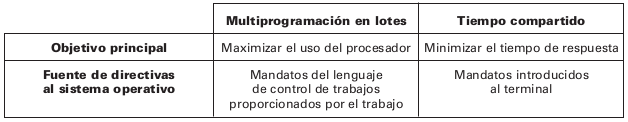
\includegraphics[width=1\textwidth, scale=1]{figura17.png}
				\end{figure}	
				
				Mencionar uno de los primeros sistemas oeprativos de tiempo comaprtido desarrollados fue el CTSS(\textit{Compatible Time-Sharing System}. Este comparado con otros posteriores es primitivo. Era extremadamente sencialla, lo que minimizaba el tamaño del monitor. Debido a que un trabajo siempre se cargaba en la misma dirección de memorio, no había necesidad de utilizar técnicas de reubicación en tiempo de carga. El hecho de sólo escribir en disco cuando es necesario, minimiza la actividad del disco. Este tenía un máximo de 32 usuarios. \\
				
				La compartición de tiempo y la multiprogramación implican nuevos problemas para el SO. Si existen múltiples trabajos en memoria, éstos deben protegerse para evitar que interfieran entre sí. Con múltiples usuarios interactivos, el sistema de ficheros debe ser protegido, de forma que sólo usuarios actualizados tengan acceso a un fichero particular. También debe gestionarse los conflictos entre los recursos, tales como impresoras y dispositivos de almacenamiento masivo.
				
		\subsection{Principales logros}
			Los sistemas operativos se encuentran entre las piezas de software más complejas jamás desarrolladas. Esto refleja el reto de intentar resolver la dificultad de alcanzar determinados objetivos, algunas veces conflictivos, de convivencia, eficiencia y capacidad de evolución. Los cinco principales avances teóricos en el desarrollo de los SO:
			
			\begin{itemize}
			\item Procesos.
			\item Gestión de memoria.
			\item Protección y seguridad de la información.
			\item Planificación y gestión de los recursos.
			\item Estructura del sistema.
			\end{itemize}
			
			\subsubsection{Procesos}
				El concepto de proceso es fundamental en la estructura de los SO. Es un término un poco más general que el de trabajo. Se han dado muchas difiniciones del término proceso, incluyendo:
				
				\begin{itemize}
				\item Un programa en ejecución.
				\item Una instancia de un programa ejecutándose en un computador.
				\item La entidad que se puede asignar o ejecutar en un procesador.
				\item Una unidad de actividad caracterizada por un solo hilo secuencial de ejcución, un estado actual, y un conjunto de recursos del sistema asociados.
				\end{itemize}
				
				Tres líneas principales de desarrollo del sistema de computación crearon problemas de temporarización y sincronización que contribuyeron al desarrollo del concepto de proceso: operación en lotes multiprogramados, tiempo compartido, y sistemas de transacciones de tiempo real. Como ya se ha visto, la multiprogramación se diseñó para permitir el uso simultáneo del procesador y los dispositivo de E/S, incluyendo los dispositivos de almacenamiento, para alcanzar la máxima eficiencia. El mecnismo clave es: en respuesta a las señales que indican la finalización de las transacciones de E/S, el procesador es planificado para los diferentes programas que residen en memoria principal. \\
				
				Una segunda línea de desarrollo fue el tiempo compartido de propósito general. En este caso, el objetivo calve de diseño es responder a las necesidades del usuario y, debido a razones económicas, ser capaz de soportar muchos usuarios simultáneamente. Estos objetivos son compatibles debido al tiempo de reacción relativamente lento del usuario. Un usuario típico necesita una media de 2 segundo de tiempo de procesamiento por minuto, entonces una cantidad de 30 usuario aproximadamente podría comaprtir el mismo sistema sin interfernecias notables. Por supuesto, la sobrecarga del sistema debe tenerse en cuenta para realizar estos cálculos. \\
				
				Otra línea importante de desarrollo han sido los sistemas de procesamiento de transacciones de tiempo real. En este caso, un cierto número de usarios realizan consultas o actualizaciones sobre una base de datos. La principal diferencia entre el sistem de procesamiento de transacciones y el sistema de tiempo real es que el primero está limitado a una o unas pocas aplicaciones, mientras que los usuarios de un sistema de tiempo real pueden estar comprometidos en el desarrollo de programas, la ejecución de trabajos, y el uso de varias aplicaciones. En ambos casos, el tiempo de respuesta del sistema es impresionante. \\
				
				La principal herramienta disponible para programadores de sistema para el desarrolo de la inicial multiprogramación y los sistemas interactivos multiusuario fue la interrupción. Cualquier trabajo podía suspender su actividad por la ocurrencia de un evento definido, tal como la finalización de una operación de E/s. El procesador guardaría alguna forma de contexto y saltaría a la rutina de tratamiento de interrupciones, que determinaría la naturalez de la interrupción, procesaría la interrupción, y después continuaría el procesamiento de usuario con el trabajo interrumpido o algún otro trabajo. \\
				
				El diseño del software del sistema para coordinar estas diversas actividades resultó ser notablemente difícil. Con la progresión simultánea de muchos trabajos, cada uno de los cuales suponía la realización de numerosos pasos para su ejecución secuencial, era imposible analizar todas las posibles combinaciones de secuencias de eventos. Con la ausencia de algún método sistemático de coordinación y cooperación entre las actividades, los programadores acudían a métodos <<\textit{ad hoc}>> basados en la comprensión del entorno que el sistema operativo tenía que controlar. Estos esfuerzos eran vulnerables frente a errores de programación sutiles, cuyos efectos sólo podían observarse cuando ciertas extrañas secuencias de acciones ocurrían. Estos errores eran difíciles de diagnosticar, porque necesitaban distinguirse de los errores de software y hardware de las aplicaciones. Incluso cuando se detectaba el error, era difícil determinar la causa, porque las condiciones precisas bajo las caules el error aparecía, eran difíciles de reproducir. Existen cuatro causas principales de dichso errores:
				
				\begin{itemize}
				\item \textbf{Inapropiada sincronización.} Es frecuente el hecho de que una rutina se suspenda esperando por algún evento en el sistema. Por ejemplo, un programa que inicia una lectura de E/S debe esperar hasta que los datos estén disponibles en un buffer antes de proceder. En este caso, se necesita una señal procedente de otra rutina. El diseño inapropiado del mecanismo de señalización puede provocar que las señales se pierdan o se reciban señales duplicadas.
				\item \textbf{Violación de la exclusión mutua.} Frecuentemente, mñas de un programa o usuario intentan hacer uso de recursos compartidos simultáneamente. Por ejemplo, dos usuario podrían intentar editar el mismo fichero a la vez. Si estos accesos no se controlan, podría ocurrir un error. Debe existir algún tipo de mecanismo de exclusión mutua que permita que sólo una rutina en un momento determinado actualice un fichero. Es difícil verificar que la implementación de la exclusión mutua es correcta en todas las posibles secuencias de eventos.
				\item \textbf{Operación no determinista de un programa.} Los resultado de un programa particular normalmente dependen sólo de la entrada a dicho programa y no de las actividades de otro programa en un sistema compartido. Pero cuando los programas comparten memoria, y sus ejecuciones son entralazadas por el procesador, podrían interferir entre ellos, sobreescribiendo zonas de memoria comunes de forma impredecible. Por tanto, el orden en el que diversos programas se planifican puede afectar a la salida de cualquier programa particular.
				
				\item \textbf{Interbloqueos.} Es posible que dos o más programas se queden bloqueados esperándose entre sí. Por ejemplo, dos programas podrían requerir dos dispositivos de E/s para llevar a cabo una operación. Uno de los programas ha tomado control de uno de los dispositivos y el otro programa tiene control del otro dispositivo. Cada uno de ellos está esperando a que el otro programa libere el recurso que no poseen. Dicho interbloqueo puede depender de la temporarización de la asignación y liberación de recursos.
				\end{itemize}
				
				Lo que se necesita para enfrentarse a estos problemas es una forma sistemática de monitorizar y controlar la ejecución de varios programas en el procesador. El concepto de proceso proporciona los fundamentos. Se puede considerar que un proceso está forma por los tres siguientes componentes:
				
				\begin{itemize}
				\item Un programa ejecutable.
				\item Los datos asociados que necesita el programa (variables, espacio de trabajo, \textit{buffers}, etc.).
				\item El contexto de ejecución del programa.
				\end{itemize}
							
					
				Este último es esencial. El \textbf{contexto de ejecución}, o \textbf{estado del proceso}, es el conjunto de datos interno por el cual el sistema operativo es capaz de supervisar y controlar el proceso. Esta información interna está separada del proceso, porque el sistema operativo tiene información a la que el proceso no puede acceder. El contexto incluye toda la información que el SO necesita para gestionar el porceso y que el procesador necesita para ejecutar el proceso apropiadamente. El contexto incluye el contenido de diversos registros del procesador, tales como contador de programa y los registros de datos. También incluye información de uso del sistema operativo, como la piroridad del proceso y si un proceso está esperando por la finalización de un evento de E/S  particular. \\
				
				Dos procesos, A y B, se encuentran en una porción de memoria principal. Es decir, se ha asignado un bloque de memroia a cada proceso, que contiene el programa, datos e información de contexto. Se incluye a cada proceso en una lista de procesos que construye y mantiene el SO. La lista de procesos contiene una entrada por proceso, e incluye un puntero a la ubicación del bloque de memoria que contiene al proceso. La entrada podría también incluir parte o todo el contexto de ejecución del proceso. El resto del contexto de ejecución es almacenado en otro lugar, tar vez junto al proceso o en una región separada de memoria. El registro índice del proceso contiene el índice del proceso que el procesador está actualmente controlando en la lista de procesos. El contador de programa apunta a la siguiente instrucción del proceso que se va a ejecutar. Los registros base y límite definen la región de memoria ocupada por el proceso: el registro base contiene la dirección inicial de la región de memoria y el registro límite el tamaño de la región. El contador de programa y todas las referencias de datos se interpretan de forma relativa al registro base y no deben exceder el valor almacenado en el registro límite. Esto previene la interferencia entre los procesos. En la figura \ref{figura18:implementaciondeprocesos} se establece un esquema de la implementación de procesos.
				
				\begin{figure}
				\caption{Implementación de procesos típica}
				\label{figura18:implementaciondeprocesos}
				\centering
				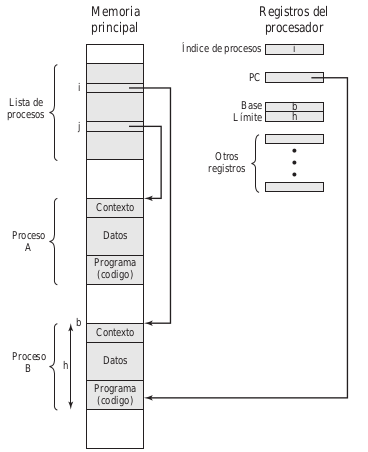
\includegraphics[width=0.8\textwidth, scale=1]{figura18.png}
				\end{figure}					
							
							
				Por tanto, el proceso puede verse como una estructura de datos. Un proceso puede estar en ejecución o esperando a ejecutarse. El \textbf{estado} completo del proceso en un instante dado se contine en su contexto. Esta estructura permite el desarrollo de técnicas potentes que aseguran la coordinación y la cooperación entre los procesos. Se pueden diseñar e incorporar nuevas características en el SO, expandiendo el contexto para incluir cualquier información nueva que se utiliza para dar soporte a dicha característica.
				
			\subsubsection{Gestión de memoria}
				Un entorno de computación que permita programación modular y el uso flexible de datos puede ayudar a resolver mejor las necesidades de los usuarios. Los gestores de sistema necesitan un control eficiente y ordenado de la asignación de los recursos. Para satisfacer estos requisitos, el SO tiene cinco responsabilidades principales de gestión de almacenamiento:
				
				\begin{itemize}
				\item \textbf{Aislamiento de procesos.} El SO debe evitar que los procesos independientes interfieran en la memoria de otro proceso, tanto datos como instrucciones.
				\item \textbf{Asignación y gestión automática.} Los programas deben tener una asignación dinámica de memoria por demanda, en cualquier nivel de la jerarquía de memoria. La asignación debe ser transparente al programador. Por tanto, el programador no debe preocuparse por los aspectos relacionados con limitaciones de memoria, y el SO puede lograr incrementar la eficiencia, asignando memoria a los trabajos sólo cuando se necesiten.
				\item \textbf{Soporte a la programación modular.} Los programadores deben ser capaces de definir módulos de programación y crear, destruir, y alterar el tamaño de los módulos dinámicamente.
				\item \textbf{Protección y control de acceso.} La compartición de memoria, en cualquier nivel de la jerarquía de memoria, permite que un programa direccione un espacio de memoria de otro proceso. Esto es deseable cuando se necesita la compartición por parte de determinadas aplicaciones. Otras veces, esta característica amenza la integriad de los programas e incluso del propio SO. El SO debe permitir que varios usuarios puedan acceder de distintas formas a porciones de memoria.
				\item \textbf{Almacenamiento a largo plazo.} Muchas aplicaciones requieren formas de almacenar la información durante largos periodos de tiempo, después de que el computador se haya apagado.
				\end{itemize}
				
				Normalmente, los SO alcanzan estos requisitos a través del uso de la memoria virutal y las utilidades de los SO. El SO implementa un almacenamiento a largo plazo, con la información almacenada en objetos denominados ficheros. El fichero es un concepto lógico, conveniente para el programador y es una unidad útil de control de acceso y protección para los SO. \\
				
				La memoria virutal es una utilidad que permite a los programas direccionar la memoria desde un punto de vista lógica, sin importar la cantidad de memoria principal física disponible. La memoria virutal fue concebida como un método para tener múltiples trabajos de usuario residiendo en memoria principal de forma concurrente, de forma que no exista un intervalo de tiempo de espera entre la ejecución de procesos sucesivos,es decir, mientras un proceso se escribe en almacenamiento secundario y se lee el proceso sucesor. Debido a que los procesos varían de tamaño, si el procesador planifica un determinado número de procesos, es difícil almacenarlos compactamente en memoria principal. Se introdujeron los sistemas de paginación, que permiten que los procesos se compriman en un número determinado de bloques de tamaño fijo, denominados páginas. Un programa referencia una palabra por medio de una \textbf{dirección virtual}, que consiste en un número de página y un desplazacmiento dentro de la página. Cada página de un proceso se puede localizar en cualquier sitio de memoria principal. El sistema de paginación proporciona una proyección dinámica entre las direcciones virtuales utilizadas por el programa y una dirección real, o dirección física, de memoria principal.	\\
				
				Con el hardware de proyección dinámica disponible, el siguiente paso era eliminar el requisito de que todas la páginas de un proceso residan en memoria principal simultáneamente. Todas las páginas de un proceso se mantienen en disco. Cuando un proceso está en ejecución, alguna de sus páginas se encuentran en memoria principal. Si se referencia una página que no está en memoria principal, el hardware de gestión de memoria lo detecta y permite que la página que false se cargue. \\
				
				El hardware del procesador, junto con el SO, dota al usuario de un <<procesador virtual>> que tiene acceso a la memoria virtual. Este almacen podría ser un espacio de almacenamiento lineal o una colección de segmentos, que son bloques de longitud variable de direcciones contiguas. En ambos casos, las instrucciones del lenguaje de programación pueden referenciar al programa y a las ubicaciones de los datos en el área de memoria virtual. El aislamiento de los procesos se puede lograr dando a cada proceso una única área de memoria virtual, que no se solape con otras áreas. La compartición de memoria se puede lograr a través de porciones de dos espacios de memoria virtual que se solapan. Los ficheros se mantienen en un almacenamiento a largo plazo. Los ficheros o parte de los mismo se pueden copiar en la memoria virtual para que los programas los manipulen.	\\
				
				El almacenamiento está compuesto por memeoria principal direccionable y memoria auxiliar de baja velocidad a la que se accede de forma indirecta, cargando bloques de la misma en memoria principal. El hardware de traducción de direcciones(\textit{memory management unit}) se interpone entre el procesador y la memoria. Los programas hacen referencia a direcciones virtuales, que son proyectadas sobre direcciones reales de memoria principal. Si una referencia a una direccioón virutal no se encuentra en memoria física, entonces una porción de los contenidos de memoria real son llevados a la memoria auxiliar y los contenidos de la memoria real que se están buscando, son llevados a memoria principal. Durante esta tarea, el proceso que generó la dirección se suspende. El diseñador del SO necesita desarrollar un mencanismo de traducción de direcciones que genere poca sobrecarga y una política de asignación de almacenamiento que minimice el tráfico entre los diferentes niveles de la jerarquía de memoria. En la figura \ref{figura19:direccionamientomemvirtual} se ve un esquema de direccionamiento de memoria virtual.
				
				\begin{figure}
				\caption{Direccionamiento de memoria virtual}
				\label{figura19:direccionamientomemvirtual}
				\centering
				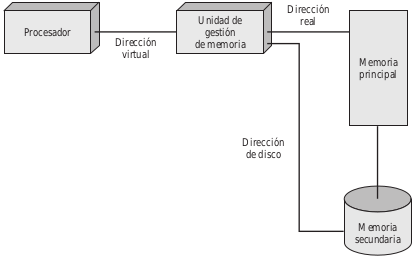
\includegraphics[width=0.8\textwidth, scale=1]{figura19.png}
				\end{figure}
				
			\subsubsection{Protección y seguridad de información}	
				El crecimiento del uso de los sistemas de tiempo compartido y, más recientemente, las redes de computadores ha originado un incremento de la preocupación por la protección de la información. La naturaleza de las amenazas que conciernen a un organización variarán enormemente dependiendo de las circunstancias. Sin embargo, hay algunas herramientas de propósito general que se pueden utilizar en los computadores y sistemas operativos para soportar una gran variedad de mecanismos de protección y seguridad. En general, el principal problema es el control del acceso a los sistemas de computación y a la información almacenada en ellos. \\
				
				La mayoría del trabajo en seguridad y protección relacionado con los sistemas operativos se puede agrupar en cuatro categorías genéricas:
				
				\begin{itemize}
				\item \textbf{Disponibilidad.} Relacionado con la protección del sistema frente a las interrupciones.
				\item \textbf{Confidencialidad.} Asegura que los usuarios no puedan leer los datos sobre los cuales no tienen autorización de acceso.
				\item \textbf{Integridad de los datos.} Protección de los datos frente a modificaciones no autorizadas.
				\item \textbf{Autenticidad.} Relacionado con la verificación apropiada de la identidad de los usuarios y la validez de los mensajes o los datos.
				\end{itemize}
				
			\subsubsection{Planificación y gestión de los recursos}
				Una responsabilidad clave de los sistemas operativos es la gestión de varios recursos disponibles para ellos y para planificar su uso por parte de los distintos procesos activos. Cualquier asignación de recursos y política de planificación debe tener en cuenta tres factores:
				
				\begin{itemize}	
				\item \textbf{Equitatividad.} Normalmente, se desea que todos los procesos que compiten por un determinado recurso, se les conceda un acceso equitativo a dicho recurso. Esto es especialmente cierto para trabajos con demandas similares.
				\item \textbf{Respuesta diferencial.} Por otro lado, el SO puede necesitar discriminar entre diferentes clases de trabajos con diferentes requisistos de servicio. El SO debe tomar las decisiones de asignación y planificación con el objetivo de satisfacer el conjunto total de requisitos. Además, debe tomar las decisiones de forma dinámica. Por ejemplo, si un proceso está esperando por el uso de un dispositivo de E/S, el SO puede intentar planificar este proceso para su ejecución tan pronto como sea posible a fin de liberar el dispositivo para posteriores demandas de otros procesos.
				\item \textbf{Eficiencia.} El SO debe intentar maximizar la productividad, minimizar el tiempo de respuesta, y, en caso de sistemas de tiempo compartido, acomodar tantos usuarios como sea posible. Estos criterios entran en conflicto; encontrar un compromiso adecuado en una situación particular es un problema objeto de la investigación sobre SO.
				\end{itemize}											
					
				La planificación y la gestión de recursos son esencialmente problemas de investigación, y se pueden aplicar los resultados matemáticos de esta disciplina. Adicionalmente, medir la actividad del sistema es importante para ser capaz de monitorizar el rendimiento y realizar los ajustes correspondientes.	
				
				El SO mantiene un numero de colas, cada una de las cuales es simplemente una lista de procesos esperando por algunos recursos. La cola a corto plazo está compuesta por procesos que se encuentran en memoria principal y están listos para ejecutar, siempre que el procesador esté disponible. Cualquiera de estos procesos podría usar el procesador a continuación. Es responsabilidad del planificador a corto plazo, o \textbf{\textit{dispatcher}}, elegir uno de ellos. Una estrategia común es asignar en orden a cada proeso de la cola un intervalo de tiempo; esta técnica se conoce como \textbf{round-robin} o \textbf{turno rotatorio}. En efecto, la técnica de turno rotatorio emplea una cola ciruclar. Otra estrategia consiste en asignar niveles de prioridad a los distintos procesos, siendo el planificador el encargado de elegir los procesos en orden de prioridad. \\
				
				La cola a largo plazo es un lista de nuevos trabajos esperando a utilizar el procesador. El sistema operativo añade trabajos al sistema transfiriendo desde la cola a largo plazo hasta la cola a corto plazo. En este punto, se debe asignar una porción de memoria principal al proceso entrante. Por tanto, el SO debe estar seguro de que no sobrecarga la memoria o el tiempo de procesamiento admitiendo demasiados procesos al sistema. Hay una cola de E/S por cada dispositivo de E/S. Más de un proceso puede solicitar el uso del mismo dispositivo de E/S. Todos los procesos que esperan utilizar dicho dispositivo, se encuentran alineados en la cola del dispositivo. De nuevo, el sistema operativo debe determinar a qué proceso le asigna un dispositivo de E/S disponible. \\
				
				Si ocurre una interrupción, el sistema operativo recibe el control del procesador a través de un manejador de interrupciones. Un proceso puede invocar específicamente un servicio del sistema operativo, tal como un manejador de un dispositivo de E/S, mediante una \textbf{llamada al sistema}. En este caso, un manejador de la llamada a sistema es el punto de entrada al sistema operativo. En cualquier caso, una vez que se maneja la interrupción o la llamada al sistema, se invoca al planificador a corto plazo para que seleccione un proceso para su ejecución. \\
				
				\begin{figure}
				\caption{Elementos clave de un SO para la multiprogramación}
				\label{figura20:elementos clave}
				\centering
				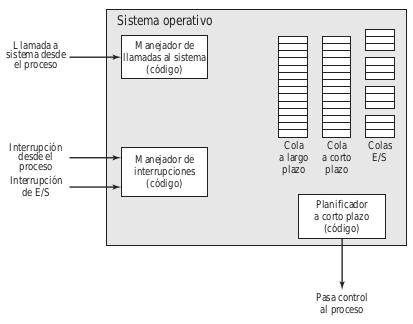
\includegraphics[width=0.8\textwidth, scale=1]{figura20.png}
				\end{figure}
				
			
			\subsubsection{Estructura del sistema}
				El tamaño de un SO con un conjunto completo de característica, y la dificultad del problema que afronta dicho sistema, ha llevado a esta disciplina a cuatro desafortunados, aunque demasiado comunes, problemas. En primer lugar, los sistemas operativos se entregan tarde de forma crónica. Esto implica la creación de nuevos sistemas operativos y frecuentes actualizaciones a viejos sistemas. En segundo lugar, los sistemas tienen fallos latentes que deben ser planteados y resuletos. En tercer lugar, el rendimiento no es frecuentemente el esperado. En último lugar, se ha comprobado que es casi imposbile construir un SO complejo que no sea vulnerable a una gran cantidad de ataques de seguridad, incluyendo virus, gusanos y accesos no autorizados. \\
				
				Para gestionar la complejidad de los sistemas operativos y eliminar estos problemas, se ha puesto mucho énfasis en la estructura software del sistema operativo a lo largo de los años. Ciertos puntos parecen obvios. El software debe ser modular. Esto ayudará a organizar el proceso de desarrollo de software y limitará el esfuerzo de diagnosticar y corregir errores. Los módulos deben tener interfaces bien definidas, y estas interfaces deben ser tan sencillas como sea posible. De nuevo, esto facilita la programación. También facilita la evolución del sistema. Con mínimas interfaces entre los módulos, se puede modificar un módulo con un mínimo impacto en otros módulos.	\\
				
				Para sistemas operativos grandes, que ejecutan desde millones a decenas de millones de líneas de código, no es suficiente la programación modular. De hecho, ha habido un incremento en el uso de los conceptos de capas jerárquicas y abstracción de información. La estructura jerárquica de un SO moderno separa sus funciones de acuerdo a las características de su escala de tiempo y su nivel de abstracción. Se puede ver el sistema como una serie de niveles. Cada nivel realiza un subconjunto relacionado de funciones requeridas por el SO. Dicho nivel confía en los niveles inmediatamente inferiores para realizar funciones más primitivas y ocultar los detalles de esas funciones. Cada nivel proporciona servicios a la capa inmediatatmente superior. Idealmente, estos niveles deben definirse de tal forma que los cambios en un nivel no requieran cambios en otros niveles. Por tanto, de esta forma se ha descompuesto un problema en un número de subproblemas más manejables.	\\
				
				En general, las capas inferiores tratan con una escala de tiempo menor. Algunas partes del SO deben interaccionar directamente con el hardware del computador, donde los eventos pueden tener una escala tan ínfima como unas pocas mil millonésimas de segundo. En el otro extremo del espectro, algunas partes del SO se comunican con el usuario, que invoca mandatos en una escala de tiempo mucho más larga, tal vez unos pocos segundos. El uso de un conjunto de niveles se adapta adecuadamente a este entorno. \\
				
				La forma en que estos principios se aplican varía enormemente entre los sistemas operativos contemporáneos. Sin embargo, es útil en este punto, para el propósito de mostrar los sistemas operativos, presentar un modelo de SO jerárquico. El modelo de define en y está compuesto por:
				
				\begin{itemize}
				\item \textbf{Nivel 1.} Está formado por cirucitos electrónicos, donde los objetos tratados son registros, celdas de memoria, y puertas lógicas. Las operaciones definidas en estos objetos son acciones, como poner a cero un registro o leer una posición de memoria.
				\item \textbf{Nivel 2.} El conjunto de instrucciones del procesador. Las operaciones a este nivel son aquellas permitidas en el conjunto de instrucciones de lenguaje máquina, como adición, resta, carga o almacenamiento.		
				\item \textbf{Nivel 3.} Añade el concepto de procedimiento o subrutina, más las operaciones de llamada y retorno (\textit{call/return}).
				\item \textbf{Nivel 4.} Introduce las interrupciones, que permiten al procesador guardar el contexto actual e invocar una rutina de tratamiento de interrupciones. \\
				
				Estos cuatro primeros niveles no son parte del SO, sino que constituyen el hardware del procesador. Sin embargo, algunos elementos del SO se empiezan a mostrar en estos niveles, por ejemplo, las rutinas de tratamiento de interrupciones.
				
				\item \textbf{Nivel 5.} En este nivel se introduce la noción de un proceso como un programa en ejecución. Los requisitos fundamentales de los sistemas operativos para dar soporte a múltiples procesos incluyen la habilidad de suspender y continuar los procesos. Esto requiere guardar los registros de hardware de forma que se puede interrumpir la ejecución de un proceso e iniciar la de otro. Adicionalmente, si los procesos necesitan cooperar, se necesitan algunos métodos de sincronización. Una de las técnicas más sencillas, y un concepto importante en el diseño de los sistemas operativos, es el semáforo.
				\item \textbf{Nivel 6.} Trata los dispositivos de almacenamiento del computador. En este nivel, se dan las funciones para posicionar las cabezas de lecturar/escritura y la transferencia real de bloques. El nivel 6 delega al nivel 5 la planificación de la operación y la notificación al proceso solicitante de la finalización de la misma. Niveles más altos se preocupan de la dirección en el disco de los datos requeridos y proporcionan una petición del bloque de datos apropiado a un controlador de dispositivo del nivel 5.
				\item \textbf{Nivel 7.} Crea un espacio de direcciones lógicas para los procesos. Este nivel organiza el espacio de direcciones virtuales en bloques que pueden moverse entre memoria principal y memoria secundaria. Tres esquemas son de uso comun: aquellos que utilizan páginas de tamaño fijo, aquellos que utilizan segmento de longitud variable y aquellos que utilizan ambos. Cuando  un bloque de memoria necesario no se encuentra en memoria principal, la lógica de este nivel requiere un transferencia desde el nivel 6. \\
				
				Hasta este punto, el sistema operativo trata con los recursos de un único procesador. A partir de aquí, el sistema operativo trata con objetos externos, como dispositivos periféricos y posiblemente redes y computadores conectados a la red. Los objetos de estos niveles superiores son bojetos lógicos con nombre, que pueden compartirse entre procesos del mismo computador o entre múltiples computadores.
				
				\item \textbf{Nivel 8.} Trata la comunicación de información y mensajes entre los procesos. Mientras que en el nivel 5 proporciona un mecanismo de señalización primitivo que permite la sincronización de procesos, este nivel trata con una compartición de información más rica. Una de las herramientas más potentes para este propósito es la tubería o \textit{pipe}, que es un canal lógico para el flujo de datos entre procesos. Una tubería se define por sus salida de un proceso y su entrada en otro proceso. Se pueden también utilizar para enlazar dispositivos externos o ficheros a procesos. 
				\item \textbf{Nivel 9.} Da soporte al almacenamiento a largo plazo en ficheros con nombre. En este nivel, los datos en el almacenamiento secundario se ven términos de entidades abstractas y con longitud variable. Esto contrasta con la visión orientada a hardware del almacenamiento secundario en términos de pistas, sectores y bloques de tamaño fijo en el nivel 6.
				\item \textbf{Nivel 10.} Proporciona acceso a los dispositivos externos utilizando interfaces estándar.
				\item \textbf{Nivel 11.} Es el nivel responsable para mantener la asociación entre los identificadores externos e internos de los recursos y objetos del sistema. El identificador externo es un nombre que puede utilizar una aplicación o usuario. El identificador interno es una dirección de otro identificador que puede utilizarse por parte de los niveles inferiores del sistema operativo para localizar y controlar un objeto. Estas asociaciones se mantienen en un directorio. Las entradas no sólo incluyen la asociación entre identificadores externos/internos, sino también características como los derechos de acceso.
				
				\item \textbf{Nivel 12.} Proporciona una utilidad completa para dar soporte a los procesos. Este nivel va más allá del proporcionado en el nivel 5. En este, sólo se mantienen los contenidos de los registros del procesador asociados con un proceso, más la lógica de los procesos de planificación. En el nivel 12, se da soporte a toda la información necesaria para las gestión ordenada de los procesos. Esto incluye el espacio de direcciones virtuales de los procesos, una lista de objetos y procesos con la cual puede interactuar y las restricciones de esta interacción, parámetros pasasdos al proceso en la creación. También se incluye cualquier otra característica que pudiera utilizar el sistema operativo para controlar el proceso.	
				
				\item \textbf{Nivel 13.} Proporciona una interfaz del SO al usuario. Se denomina \textbf{\textit{shell}}, porque separa al usuario de los detalles de los sistemas operativos y presenta el sistema operativo simplemente como una colección de servicios. El \textit{shell} acepta mandatos de usuario o sentencias de control de trabajos, los interpreta y crea y controla los procesos que necesita para su ejecución. Por ejemplo, a este nivel la interfaz podría implementarse como un menú y mostrando los resultados utilizando una salida gráfica conectada a un dispositivo específica, tal y como una pantalla.			
				\end{itemize}
				
				Este modelo hipotétio de un SO proporciona una estructura descriptiva útil y sirve como una guía de implementación. 
				
				\begin{figure}
				\caption{Jerarquía de diseño del SO}
				\label{figura21:jerarquiadiseño}
				\centering
				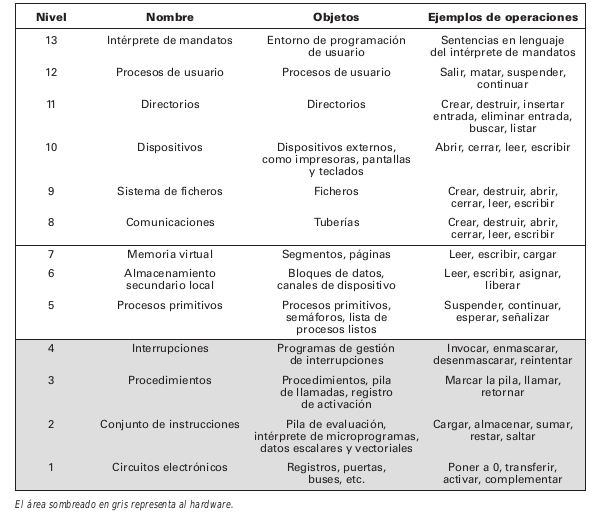
\includegraphics[width=1.1\textwidth, scale=1]{figura21.png}
				\end{figure}
				
			
		\subsection{Desarrollos que han llevado a los sistemas operativos modernos}
			La velocidad de cambio en las demandas de los sistemas operativos requiere no sólo modificaciones o mejoras en arquitecturas existentes sino también nuevas formas de organizar el sistema operativo. Un amplio rango de diferentes técnicas y elementos de diseño se han probado tanto en sistemas operativos experimentales como comerciales, pero la mayoría de este trabajo encaja en las siguientes categorías:
			
			\begin{itemize}
			\item Arquitectura micronúcleo o \textit{microkernel}.
			\item Multihilo.
			\item Multiprocesamiento simétrico (SMP).
			\item Sistemas operativos distribuidos.
			\item Diseño orientado a objetos.
			\end{itemize}
			
			Hasta hace relativamente poco tiempo, la mayoría de los sistemas operativos estaban formados por un gran \textbf{núcleo monolítico}. Estos grande núcleos proporcionan la mayoría de las funcionalidades consideradas propias del sistema operativo, incluyendo la planificación, los sistemas de ficheros, las redes, los controladores de dispositivos, la gestión de memoria y otras funcioens. Normalmente, un núcleo monolítico se implementa como un único proceso, con todos los elementos compartiendo el mismo espacio de direcciones. Una \textbf{arquitectura micronúcleo} asigna sólo unas pocas funciones esenciales al núcleo, incluyendo los espacios de almacenamiento, comunicación entre procesos (IPC), y la planificación básica. Ciertos procesos proporcionan otros servicios del SO, algunas veces denominados servidores, que ejecutan en modo usuario y son tratados como cualquier otra aplicación por el micronúcleo. Esta técnica descopla el núcleo y el desarrollo del servidor. Los servidores pueden configurarse para aplicaciones específicas o para determinados requisitos del entorno. Los servidores pueden configurarse para aplicaciones específicas o para determinados requisitos de entorno. La técnica micronúcleo simplifica la implementación, proporciona flexibilidad y se adapta perfectamente a un entorno distribuido. En esencia, un micronúcleo interactúa con procesos locales y remotos del servidor de la misma forma, facilitando la construcción de los sistemas distribuidos. \\
			
			\textbf{Multithreading} es una técnica en la cual un proceso, ejecutando una aplicación, se divide en un serie de hilos o \textit{threads} que pueden ejecutar concurrentemente. Se pueden hacer las siguientes distinciones:
			
			\begin{itemize}
			\item \textbf{Thread o hilo.} Se trata de una unidad de trabajo. Incluye el contexto del procesador (que contiene el contador del programa y el puntero de pila) y su propia área de datos para una pila (para posibilitar el salto a subrutinas). Un hilo se ejecuta secuencialmente y se puede interrumpir de forma que el procesador pueda dar paso a otro hilo.
			\item \textbf{Proceso.} Es una colección de uno o más hilos y sus recursos de sistema asociados (como la memoria, conteniendo tanto código, como datos, ficheros abiertos y dispositivos). Esto corresponde al concepto de programa de ejecución. Dividiendo una sola aplicación en múltiples hilos, el programador tiene gran control sobre la modularidad de las aplicaciones y la temporarización de los eventos relacionados con la aplicación.
			\end{itemize}
			
			La técnica \textit{multithreading} es útil para las aplicaciones que llevan a cabo un número de tareas esencialmente independientes que no necesitan ser serializadas. Un ejemplo es un servidor de bases de datos que escucha y procesa numerosas peticiones de cliente. Con múltiples hilo ejecutándose dentro del mismo proceso, intercambiar la ejecución entre los hilos suponen menos sobrecarga del procesador que intercambiar la ejecución entre diferentes procesos pesados. Los hilos son también útiles para estructurar procesos que son parte del núcleo del SO. \\
			
			A medida que la demanda de rendimiento se incrementa y el coste de los microprocesadores continúa cayendo, los fabricantes han introducido en el mercado computadores con múltiples procesadores. Para lograr mayor eficiencia y fiabilidad, una técnica consiste en emplear \textbf{multiprocesamiento simétrico (	SMP: \textit{Symmetric Multi-Processing}}), un término que se refiere a la arquitectura hardware del computador y también al comportamiento del SO que explota dicha arquitectura. Se puede definir un multiprocesamiento simétrico como un sistema de computación aislado con las siguientes características:
			
			\begin{enumerate}
			\item Tiene multiples procesadores.
			\item Estos procesadores comparten las mismas utilidades de memoria principal y de E/S, interconectadas por un bus de comunicación u otro esquema de conexión interna.
			\item Todos los procesadores pueden realizar las mismas funciones.
			\end{enumerate}
			
			El SO de un SMP planifica procesos o hilos a través de todos los procesadores. SMP tiene diversas ventajas potenciales sobre las arquitecturas monoprocesador, entre las que se incluyen:
			
			\begin{itemize}
			\item \textbf{Rendimiento.} Si el trabajo se puede organizar de tal forma que alguna porción del trabajo se pueda realizar en paralelo, entonces un sistema con múltiples procesadores alcanzará mayor rendimiento que uno con un solo procesador del mismo tipo. Con la multiprogramación, sólo un proceso puede ejecutar a la vez; mientras tanto, el resto de procesos esperan por el procesador. Con multiproceso, más de un proceso puede ejecutarse simultáneamente, cada uno de ellos en un procesador diferente.
			\item \textbf{Disponibilidad.} En un multiprocesador simétrico, debido a que todos los procesadores pueden llevar a cabo las mismas funciones, el fallo de un solo procesador no para la máquina. Por el contrario, el sistema puede continuar funcionando con un rendimiento reducido.
			\item \textbf{Crecimiento incremental.} Un usuario puede mejorar el rendimiento de un sistema añadiendo un procesador adicional.
			\item \textbf{Escalado.} Los fabricantes pueden ofrecer un rango de productos con diferente precio y caraterísticas basadas en el número de procesadores configurado en el sistema.
			\end{itemize}	
			
			Es imporatnte notar que estas características son beneficios potenciales, no garantizados. El sistema operativo debe proporcionar herramientas y funciones para explotar el paralelismo en un sistema SMP.	\\
			
			\begin{figure}
			\caption{Multiprogramación y multiproceso}
			\label{figura22:multiprogramacion_multiproceso}
			\centering
			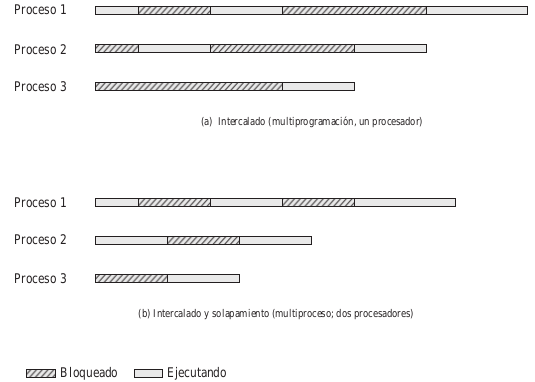
\includegraphics[width=1\textwidth, scale=1]{figura22.png}
			\end{figure}
			
			La técnica \textit{multithreading} y SMP son frecuentemente anilizados juntos, pero son dos utilidades independientes. Incluso en un nodo monoprocesador, la técnica multithreading es útil para estructurar aplicaciones y procesos de núcleo. Una máquina SMP es útil incluso para procesos que no contienen hilos, porque varios procesos se pueden ejecutar en paralelo. Sin embargo, ambas utilidades se complementan y se pueden utilizar de forma conjunta efectivamente. \\
			
			Una característica atractiva de un SMP es que la existencia de múltiples procesadores es transparente al usuario. El SO se encarga de planificar los hilos o procesos en procesadores individuales y de la sincronización entre los procesadores. Un problema diferente es proporcionar la apariencia de un solo sistema a un clúster de computadores separado-un sistema multicomputador. En este caso , se trata de una colección de entidades cada uno con sus propios módulos de memoria principal, de memoria secundaria y otros módulos de E/S. \\
			
			Un \textbf{sistema operativo distribuido} proporciona la ilusión de un solo espacio de memoria principal y un solo espacio de memoria secundario, más otras utilidades de acceso unificadas, como un sistema de fichero distribuido. \\
			
			Otra innovación en el diseño de los sistemas operativos es el uso de tecnologías orientadas a objetos. El \textbf{diseño orientado a objetos} introduce una disciplina al proceso de añadir modulares a un pequeño núcleo. A nivel de SO, una estructura basada en objetos permite a los programadores personalizar un SO sin eliminar la integridad del sistema. La orientación a objetos también facilita el desarrollo de herramientas distribuidas y sistemas operativos distribuidos.
			
		\subsection{Sistemas Unix tradicionales}
			\subsubsection{Descripción}
				En la figura \ref{figura23:arquitectura unix} se muestra una descripición general de la arquitectura UNIX. El hardware subyacente es gestionado por el software del SO. El SO se denomina frecuentemente el núcleo del sistema, o simplemente núcleo, para destacar su aislamiento frente a los usuarios y a las aplicaciones. De aquí en adelante a esta porción se la denominará como UNIX. Sin embargo, UNIX viene equivado con un conjunto de servicios de usuario e interfaces que se consideran parte del sistema. Estos se pueden agrupar en el \textit{shell}, otro software de interfaz, y los componentes del compilador C. La capa externa está formada por las aplicaciones de usuario y la interfaz de usuario del compilador C. \\
				
				\begin{figure}
				\caption{Arquitectura general de UNIX}
				\label{figura23:arquitectura unix}
				\centering
				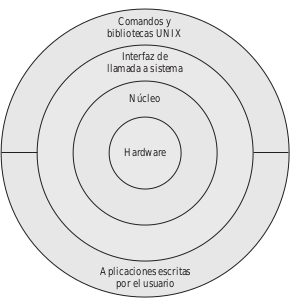
\includegraphics[width=0.6\textwidth, scale=1]{figura23.png}
				\end{figure}
				
				Los programas de usuario pueden invocar a los servicios del sistema operativos directamente o a través de programas de biblioteca. La interfaz de llamada a sistemas es la frontera con el usuario y permite que el software de alto nivel obtenga acceso a funciones específicas del núcleo. En el otro extremo, el SO contiene rutinas primitivas que interaccionan directamente con el hardware. Entre estas dos interfaces, el sistema se divide en dos partes principales, una encargada del control de procesos y la otra encargada de la gestión de fichero de la E/S. El subsistema de control de procesos se encarga de la gestión de memoria, la planificación y ejecución de los procesos, así como de la sincronización y la comunicación entre los procesos. El sistema de ficheros intercambia datos entre la memoria y los dispositivos externos tanto  flujos de caracteres como bloques. Para lograr esto, se utilizan una gran variedad de controladores de dispositivos. Para las tranferencias orientdas a bloque, se utiliza una técnica de cahce de discos: entre el espacio de direccionamiento del usuario y el dispositivo externo se interpone un \textit{buffer} de sistema en memoria principal. \\
				
				Los sistemas UNIX se diseñaron para ejecutar sobre un único procesador y carecene de la capacidad para proteger sus estructuras de datos del acceso concurrente por parte de múltiples procesadores. Su núcleo no es muy versátil, soportando un único tipo de sistema de ficheros, una única política de planificación de procesos y un único formato de fichero ejecutable. El núcleo tradicional de UNIX no está diseñado para ser extensible y tiene pocas utilidades para la reutilización de código. El resultado es que, según se iban añadiendo nuevas características a varias verisones de UNIX, se tuvo que añadir mucho código, proporcionando un núcleo de gran tamaño y no modular.
				
				\begin{figure}
				\caption{Núcleo tradicional de UNIX}
				\label{figura24:nucleoUNIX}
				\centering
				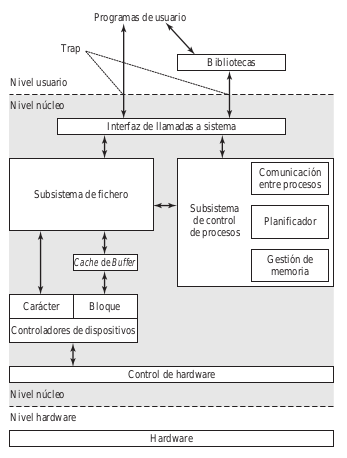
\includegraphics[width=1.1\textwidth, scale=1]{figura24.png}
				\end{figure}
				
				En la figura \ref{figura24:nucleoUNIX} se muestra un esquema del núcelo tradicional de UNIX.
				
		\subsection{Sistemas unix modernos}
			Cuando UNIX evolucionó, un gran número de diferentes implementaciones proliferó, cada una de las caules proporcionó algunas características útiles. Fue necesario de una nueva implementación que unificara muchas de las imortantes innovaciones, añadiera otras características de diseño de los sistemas operativos modernos, y produjera una arquitectura más modular. Existe un pequeño núcleo de utilidades, escritas de forma modular, que proporciona funciones y servicios necesarios para procesos del sistema operativo.
			
			\begin{figure}
			\caption{Núcleo UNIX moderno}
			\label{figura25:nucleomoderno}
			\centering
			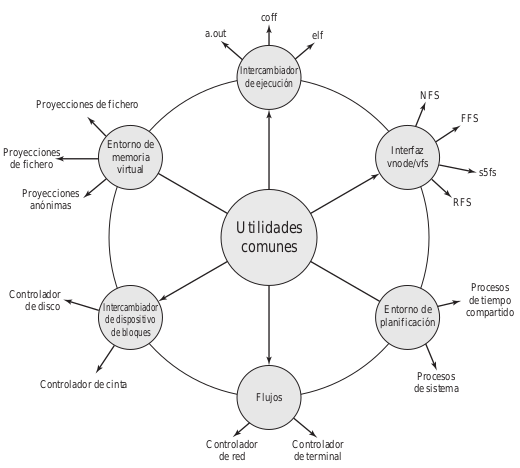
\includegraphics[width=0.8\textwidth, scale=1]{figura25.png}
			\end{figure}
			
			\subsubsection{System V relesase 4 (SVR4)}
				SVR4, desarrollado conjuntamente por AT\& T y Sun Microsistemas, combina características de SVR3, 4.3BSD, Microsoft Xenix System y SunOS. Fue casi una reescritura completa del núcleo del System V y produjo una implmentación bien organizada, aunque compleja. Las nuevas características de esta versión incluyen soporte al procesamiento en timepo real, clases de planificación de procesos, estructuras de datos dinámicamente asignadas, gestión de memoria virtual, sistema de ficheros virtual y un núcleo expulsivo. \\
				
				SVR4 mezcló los esfuerzos de los diseñadores comerciales y académicos y se desarrolló para proporcionar una plataforma uniforme que permitiera el despegue comercial de UNIX. Incorpora la mayoría de las características importantes de cualquier sistema UNIX y lo hace de una forma integrada y comercialmente viable.
				
			\subsubsection{SOLARIS 9}
				Solaris es una versión UNIX de Sun vasada en SVR4. La última versión es la 9 y proporciona todas las características de SVR4 más un conjunto de características avanzadas, como un núcleo multhilio, completamente expulsivo, con soporte completo para SMP, y una interfaz orientada a objetos para los sistemas de ficheros. Solaris es la implementación UNIX más uitlizada y comercialmente más existosa. 
			
			\subsubsection{4.4BSD}
				Las series de UNIX BSD(\textit{Berkeley Software Distribution}) han jugado un papel importante en el desarrollo de la teoría de diseño de los sistemas operativos. 4.xBSD se ha utilizado ampliamente en instalaciones académicas y ha servido como base de algunos productos comerciales UNIX. Es probable que BSD es seguramente responsable de gran parte de la popularidad de UNIX y que la mayoría de las mejoras de UNIX aparecieron en primer lugar en las versiones BSD. \\
				
				4.4BSD fue la versión final de BSD que Berkeley produjo, disolviendose posteriormente la organización encargada del diseño e implementación. Se trata de una actualización importante de 4.3BSD, que incluye un nuevo sistema de memoria virtual, cambios en la estructura del núcleo, y una larga lista de mejoras.
				
		\subsection{Linux}
			\subsubsection{Estructura modular}
				La mayoría de los núcleos de Linux son monolíticos. Un núcleo monolítico es aque que incluye prácticamente toda la funcionalidad del sistema operativo en un gran bloque de código que ejecuta como un único proceso con un único espacio de direccionamiento. Todos los componenetes funcionales del núcleo tienen acceso a todas las estructuras internas de datos y rutinas. Si los cambios se hacen sobre cualquier porción de un sistema operativo monolítico, todos lo módulos y rutinas deben volverse a enlazar y reinstalar, y el sistema debe ser reiniciado para que los cambios tengan efecto. Como resultado, cualquier modificación es difícil. Este problema es espcialmente agudo para Linux, cuyo desarrollo es global y ha sido realizado por un grupo de programadores independientes asociados de forma difusa. \\
				
				Aunque Linux no utiliza una técnica de micronúcleo, logra muchas de las ventajas potenciales de esta técnica por medio de su arquitectura modular particular. Linux está estructurado como una colección de módulos, algunos de los cuales pueden cargarse y descargarse automáticamente bajo demanda. Estos bloques relativamente independientes se llaman \textbf{módulos cargables}. Esencialmente, un módulo es un fichero cuyo código puede enlazarse y desenlazarse con el núcleo en tiempo real. Normalmente, un moulo implementa algunas funciones específicas, como un sistema de ficheros, un controlador de dispositivo o algunas características de la capa superior del núcleo. Un módulo no se ejcuta como su propio proceso o hilo, aunque puede crear los hilos del núcleo que necesite por varios propósitos. En su lugar, un módulo se ejecuta en modo núcleo en nombre del proceso actual. \\
				
				Por tanto, aunque Linux se puede considerar monolítico, su estructura modular elimina algunas de las dificultades para desarrollar y evolucionar el núcleo.
				
				Características importantes de lso modulos cargables:
				\begin{itemize}
				\item \textbf{Enlace dinámico.} Un módulo de núcelo puede cargarse y enlazarse al núcleo mientras el núcleo está en memoria y ejecutándose. Un módulo también puede desenlazarse y eleminarse de la memoria en cualquier momento.
				\item \textbf{Módulos apilables.} Los módulos se gestionan como una jerarquía. Los módulos individuales sirven como bibliotecas cuando los módulos cliente los referencian desde la parte superior de la jerarquía, y actúan como clientes cuando referencian módulos de la parte inferior de la jerarquía.
				\end{itemize}
				 					
				El enlace dinámico facilita la configuración y reduce el uso de la memoria del núcleo. En Linux, un programa de usuario o un usuario puede cargar y descargar explícitamente módulos del núcleo utilizando los mandatos insmod y rmmod. El núcleo mismo detecta la necesidad de funciones particulares y puede cargar y descargar módulos cuando lo necesite. Con módulo apilables, se pueden definir dependencias entre los módulos. Esto tiene dos ventajas: 
				 
				\begin{enumerate}
				\item El código común para un conjunto de módulos similares se puede mover a un único módulo, reduciendo la replicación.
				\item El núcleo puede asegurar que los módulos necesarios están presentes, impidiendo descargar un módulo del cual otros módulos que ejecutan dependen y cargando algunos módulos adicionalmente requeridos cuando se carga un nuevo módulo.
				\end{enumerate}
				
			\subsubsection{Componentes del núcleo}
				\begin{figure}
				\caption{Componentes del núcleo de Linux}
				\label{figura26:componentes_nucleo}
				\centering
				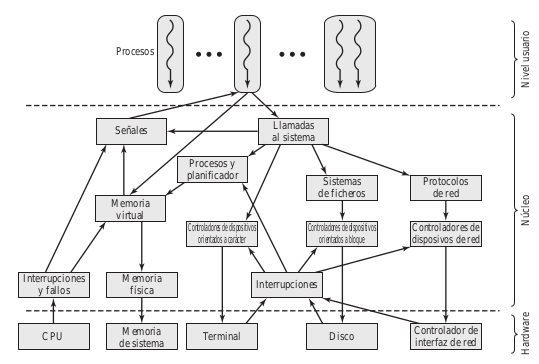
\includegraphics[width=0.8\textwidth, scale=1]{figura26.png}
				\end{figure}
				
				Usaremos la figura \ref{figura26:componentes_nucleo}. La figura muestra varios procesos ejecutando encima del núcelo. Cada caja indica un proceso separado, mientras que cada línea curvada con una cabez de flecha representa un hilo de ejecución. \\
				
				El núcleo mismo está compuesto por una colección de componentes que interaccionan, usando flechas para indicar las principales interacciones. También se muestra el hardware subyacente como un conjunto de componentes utilizando flechas para indicar qué componentes del núcleo utilizan o controlan qué componentes del hardware. Todos los componenetes del núcelo, por supuesto, ejecutan en la CPU, pero por simplicidad no se muestran estas relaciones.
				
				\begin{itemize}
				\item \textbf{Señales.} El núcleo utiliza las señales para llamar a un proceso. Por ejemplo, las señales se utilizan para notificar ciertos fallos a un proceso como por ejemplo, la división por cero.
				\item \textbf{Llamadas al sistema.} La llamada al sistema es la forma en la cual un proceso requier un servicio de núcleo específica. Hay varios cientos de llamadas al sistema, que pueden agruparse básicamente en seis categorías: sistema de ficheros, proceso, planificación, comunicación entre procesos, \textit{socket}(red) y misceláneos.
				\item \textbf{Procesos y planificador.} Crea, gestiona y planifica procesos.
				\item \textbf{Memoria virtual.} Asigna y gestiona la memoria virtual para los procesos.
				\item \textbf{Sistemas de ficheros.} Proporciona un espacio de nombres global y jerárquico para los ficheros, directorios y otros objetos relacionados con los ficheros. Además, proporciona las funcionas del sistema de ficheros.
				\item \textbf{Protocolos de red.} Da soporte a la interfaz \textit{Socket} para los usuarios, utilizando la pila de protocolos TCP/IP.
				\item \textbf{Controladores de dispositivo tipo caracter.} Gestiona los dispositivos que requier el núcleo para enviar o recibir datos de un byte cada vez, como los terminales, los módems y las impresoras.
				\item \textbf{Controladores de dispositivo tipo bloque.} Gestiona dispositivos que leen y escriben datos en bloques, tal como varias formas de memoria secundaria.
				\item \textbf{Controladores de dispositivo de red.} Gestiona las tarjetas de interfaz de red y los puertos de comunicación que permiten las conexiones a la red, tal como los puentes y los encaminadores. 
				\item \textbf{Traps y fallos.} Gestiona los traps y fallos generados por la CPU, como los fallos de memoria.
				\item \textbf{Memoria física.} Gestiona el conjunto de marcos de páginas de memoria real y asigna las páginas de memoria virtual.
				\item \textbf{Interrupciones.} Gestiona las interrupciones de los dispositivos periféricos.
				\end{itemize}
				
	\section{Virtualización}
		El término de virtualización se usó en 1960 para referirse a una máquina virtual, entendida como un duplicado aislado de un computador real.
		
		Un VM es capaz de usar los recursos del hardware vitualizados por el Virtual Machine Monitor (VMM). Un 	VMM o hipervisor es el software que proporciona la abstracción de la máquina real a las VMs. \\
		
		Los requisitos para que un hardware soporte virtualización son:
		
		\begin{itemize}
		\item \textbf{Equivalencia.} Un programa ejecutándose sobre un hipervisor debe comportarse de forma idéntica a como lo haría si se ejecutáse en la máquina física real.
		\item \textbf{Control de recursos.} El hipervisor es el único software que controla los recursos virtualizados.
		\item \textbf{Eficiencia.} La mayor proporción de instrucciones deben ejecutarse sin la intervención del hipervisor.
		\end{itemize}	
		
		\subsubsection{Tipos de virtualización}
			\textbf{Hipervisor y máquinas virutales.} Es la capa de software (hipervisor) que proporciona los recursos virtuales a las máquinas virtuales.
			
			\textbf{OS-level virtualization.} El kernel permite  múltiples instancias aisladas a nivel usuario (containers). Un programa no verá todos los recursos del SO sino solamente los asignados al container.	
		
		\subsubsection{Hipervisor y máquinas virtuales}
			La virtualización actualmente se entiende como una capa de abstracción software situada entre el software a ejecutar y el hardware real.
			
			El hipervisor crea un entorno de trabajo, la VM, para el software a ejecutar. 
			
			El hipervisor puede ser software, firmware o hardware y el ordenador en el que se ejecuta se denomina host machine, y cada máquina virtual se denomina guest machine.
			
			Más recientemente, el desarrollo y gestión de hipervisores y VMs se denomina platform virtualization o server virtualization.
			
			La virtualización permite que un único ordenador ejecute distintos SOs o múltiples ejecuciones del mismo SO.
			
			La máquina virtual dispone de una serie de recursos virtuales proporcionados por el hipervisor y sobre ella se ejecuta el SO, las bibliotecas y las aplicaciones.
			
			El ratio de consolación indica el número de VM que proporciona un determinado hipervisor.
		
		\subsubsection{Tipos de hipervisor desde Popek y Goldberg}
			\begin{itemize}
			\item \textbf{Tipo 1, native o bare-metal.} Se ejecutan directamente en el host hardware para proporcionar VM a los SO invitados.
			\item \textbf{Tipo 2, hosted.} Se ejecutan sobre un SO convencional como el resto de programas y el SO invitado se ejecuta sobre la abstracción proporcionada por el hipervisor.
			\end{itemize}
			
		\subsubsection{Razones para virtualizar}
			\begin{itemize}
			\item Permitir ejecutar diferentes SOs en el mismo HW fue el primer objetivo.
			
			Consolidación de servidores. Un HW servidor se virtualiza y tienes distintos SO actuando como servers en distintas VM.
			
			Desarrollo de kernle. VM es más fácil de controlar y observar que un HW real.
			
			VM relocation. VM con aplicaciones se traslada completamente a otro HW real.
			
			Evaluación de distintos SOs
			\end{itemize}
			
		\subsubsection{Implementación}
			El hipervisor traduce las peticiones sobre los recursos virtuales que proporciona a peticiones sobre los recursos reales del hardware. Esta traducción provoca degradación del rendimiento. 
			
			Una VM se presenta mediante archivos:
			
			\begin{itemize}
			\item Archivo de configuración: CPUs, memoria, dispositivos E/S accesibles, etc.
			\item Archivos de almacenamiento: discos virtuales y su correspondiente soporte mediante archivos reales.
			\end{itemize}
			
		\subsubsection{Funciones del hipervisor}
			\begin{itemize}
			\item Gestión de la ejecución de MVs:
				\begin{itemize}
				\item Planificación de VMs para ejecución en CPU.
				\item Gestión de la memoria virtual para aislar VMs.
				\item Cambio de contexto y emulación de timer e interrupciones.
				\end{itemize}
				
			\item Emulación de dispositivos y control de acceso.
			\item Ejecución de instrucciones privilegiadas.
			\item Gestión de máquinas virtuales
			\item Administración del hipervisor
			\end{itemize}
			
		\subsubsection{Comparación hipervisores tipo 1 y tipo 2}
			Los hipervisores tipo 1 tienen un mejor rendimiento que los de tipo 2 ya que disponen de todos los recursos de las VM y los múltiples niveles de abstracción entre el SO y el hardware real no permiten un alto rendimiento de la máquina virutal.
			
			Los hipervisores tipo 2 permiten realizar virtualización sin tener que dedicar toda la máquina a dicho fin.
			
		\subsubsection{HW-assisted virtualization}
			Arquitectura x86 no soportaba HW-assisted virtualization por lo que se desarrollaron soluciones software. El problema es que los SOs que se ejecutan sobre las máquinas virtuales necesitan ejecutarse en ring 0...
			
			Paravitualización. Es una técnica en la que el hipervisor proporciona una API y el SO que se ejecuta en una VM utiliza dicha API.
			
			Implementaciones: \\
			
				\begin{itemize}
				\item El códgio del guest OS debe estar disponible.
				\item Reemplazar instrucciones que necesitan ring 0 por hypercalls.
				\item Recompilar el guest kernel y usarlo.
				\end{itemize}
			
			Full virtualization. Esta técnica fue implementada en la primer generación VMM en x86.
			
			La idea es traducción binaria para atrapar y virtualizar la ejecución de instrucciones sensibles (ring 0).
			
			Las instrucciones sensibles se detectan (estática o dinámicamente) y se reemplazan con trampas al VMM.
			
			Esta técnica pued propovar sobrecarga del rendimiento con respecto a una VM que se ejecute en HW que soporte virtualización. \\
			
			Solución final: Intel y AMD presentan HW que soporta virtualización. Cada elemento HW debe poder ser porporcionado por hipervisor mediante una VM. El hipervisor tipo 1 debe proporcionar:
			
			 \begin{itemize}
			 \item Almacenamiento independiente de SO para proporcionar recursos a las VM.
			 \item Switching de Virtual environments para asignar recursos gestionados por el hipervisor.
			 \end{itemize}
			 
		\subsubsection{Os-level virtualization}
			\textbf{Containers.} Los container proporcionan un entorno aislado para la ejecución de programas sobre el mismo SO. Linux \textit{kernel control group}(cgroup). Permite la agrupación de procesos y gestión de recursos del sistema. Cgroup permite que distintas jerarquías de procesos coexsistean en el mismo SO. A cada jerarquía se la asigna un conjunto de recursos del sistema:
				
				\begin{itemize}
				\item Memoria máxima.
				\item Prioridad para CPU.
				\item Prioridad para dispositivos de E/S.
				\end{itemize}
				
			\textbf{Linux Namespaces.} Un espacio de nombre permite hacer visibles ciertos recursos del kernel de forma única de dicho espacio. Algunos espacios de nombres inlcuidos actualmente:
			
				\begin{itemize}
				\item System V IPC y POSIX message queues.
				\item Mounts. Sistema de archivos montado
				\item PID. Espacio de nombre para identificadores de procesos
				\item UID. Permite limitar los recursos por usuario.
				\end{itemize}
				
		\subsubsection{UML y KMV}
			\textbf{UML.} El SO anfitrión es un kernel modificado que contiene extensiones para controlar múltiples máquinas virutales cada una con su SO invitado. \\
			
			\textbf{KVM, Kernel-based Virtual Machine.} Es una implementación full virtualization para Linux sobre HW x86 que contenga las extensiones Intel VT o AMD-V.											
			
	\section{Hilos,SMP y micronúcleos}
		\subsection{Micronúcleos}
			Un micronúcleo es la pequeña parte central de un SO que proporciona las bases para extensiones modulares. Sin embargo, el término es algo confuso, y hay varias cuestiones relacionadas con los micronúcleos con respuestas distintas por parte de diferentes equipos de diseño de SOs. Estas inlcuyen, como de pequeño debe ser un núcelo para ser micronúcleo, como diseñar manejadores de dispositivos para obtener el mejor rendimientos \ldots . \\
			\subsubsection{Arquitectura micronúcleo}
				Los primeros SOs desarrollados a mediados y finales de los años 50 fueron diseñados sin preocuparse por su arquitectura. Nadie tenía la experiencia necesaria en construcción de sistemas de software realmente grandes, y los problemas causados por la dependencia mutua e interacción no se tenían en cuenta. En estos sistemas operativos monolíticos de prácticamente cualquier procedimiento se podía llamar a cualquier otro. Esta falta de estructura se hizo insostenible a medida que los sistemas operativos crecieron hasta proporciones desmesuradas. Se necesitaron técnicas de programación modular para manejar esta escala de desarrollo software. Específicamente, se desarrollaron los sistemas operativos por capas en los cuales las funciones se organizan jerárquicamente y sólo hay interacción entre las capas adyacentes. Con el enfoque por capas, la mayor parte o todas las capas ejecutan en modo núcleo. \\
				
				Los problemas permanecen incluso en el enfoque por capas. Cada capa posee demasiada funcionalidad y grandes cambios en una capa pueden tener numerosos efectos, muchos difíciles de seguir, en el código de las capas adyacentes. Como resultado es difícil implementar versiones a medida del sistema operativo básico con algunas funciones añadidas o eliminadas. Además, es difícil construir la seguridad porque hay muchas interacciones entre capas adyacentes. \\
				
				La filosofía existente en le micronúcleo es que solamente las funciones absolutamente esenciales del sistema operativo están en el núcleo. Los servicios y aplicacioens menos esenciales se construyen sobre el micronúcleo y se ejecutan en modo usuario. Aunque la filosofía de qué hay dentro y qué hay fuera del micronúclea varía de un diseño a otro, la característica general es que muchos servicios que tradicionalmente habían formado parte del SO ahora son subsistema externos que interactúan con el núcleo y entre ellos mismos (manjeadores de dispositivos, servidores de archivos, gestores de memoria virtual \ldots). \\
				
				\begin{figure}
				\caption{Arquitectura del núcleo}
				\label{figura27:arquitecturanucleo}
				\centering
				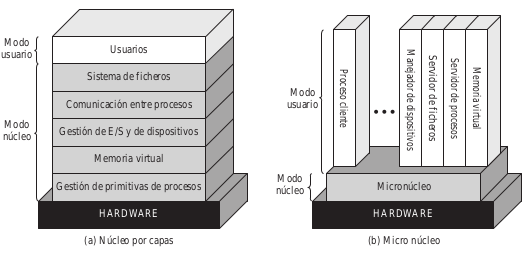
\includegraphics[width=1.1\textwidth, scale=1]{figura27.png}
				\end{figure}
				
				La arquitectura del micronúcleo reemplaza la tradicional estructura vertical y estratificada en capas por una horizontal (Figura \ref{figura27:arquitecturanucleo}b). Los componentes del SO externos al micronúcleo se implementan como servidores de procesos; interactúan entre ellos dos a dos, normalmente por paso de mensajes a través del micronúcleo. De esta forma, el micronúcleo funciona como un intercambiador de mensajes: valida mensajes, los pasa entre componentes y concede acceso al hardware. El micronúcleo también realiza una función de protección; previene el paso de mensajes a no ser que el intercambio esté permitido. \\
				
				Por ejemplo, si una aplicación quiere abrir un archivo, manda un mensaje al servido del sistema de archivos. Si quiere crear un proceso o hilo, manda un mensaje al servidor de procesos. Cada uno de los servidores puede mandar mensajes al resto de los servidores y puede invocar funciones primitivas del micronúcleo. Es decir, es una arquitectura cliente/servidor dentro de un sólo computador.
			
			\subsubsection{Beneficios de una organización micronúcleo}
				\begin{itemize}
				\item Interfaces uniformes
				\item Extensibilidad
				\item Portabilidad
				\item Fiabilidad
				\item Soporte de sistemas distribuidos
				\item Soporte de SO orientados a objetos
				\end{itemize}
				
				El micronúcleo impone una \textbf{interfaz uniforme} en las peticiones realizadas por un proceso. Los procesos no necesitan diferenciar entre servicios a nivel núcleo y a nivel usuario, porque todos los servicios se proporcionan a través de paso de mensajes. \\
				
				De forma inevitable, un SO tendrá que adquirir nuevas características que no estan en su diseño actual, a medidad que se desarrollen nuevos dispositivos hardware y nuevas técnicas software. La arquitectura micronúcleo facilita la \textbf{extensibilidad}, permitiendo agregar nuevos servicios, así como la realización de múltiples servicios en la misma área funcional. De esta forma los usuarios pueden elegir, de una variedad de servicios, el que mejor se adapte a sus necesidades. Con la arquitectura micronúcleo, cuando se añade una nueva caracterísitca, sólo el servidor relacioonado necesita modificarse o añadirse. El impacto de un servidor nuevo o modificado se restringe a un subconjunto del sistema. Además, las modificaciones no requieren la construcción de un nuevo núcleo. \\
				
				Relacionado con la extensibilidad de una arquitectura micronúcleo está su flexibilidad. No sólo se pueden añadir nuevas caracterísitcas al SO, además las características existentes se pueden eliminar para realizar una implementación más pequeña y más eficiente. U SO micronúcleo no es necesariamente un sistema pequeño. De hecho, su propia estructura le permite añadir un amplio rango de características. \\
				
				La portabilidad se convierte en una característica interesante en los SOs. En la arquitectura micronúcleo, todo o gran parte del código específico del procesador está en el micronúcleo. Por tanto, los cambios necesarios para transferir el sistema a un nuevo procesador son menores y tienden a estar unidos en grupo lógicos. \\
				
				Mayor sea el tamaño del producto software, mayor es la dificultad de asegurar su fiabilidad. Aunque el diseño modular ayuda a mejorar la fiabilidad, con una arquitectura micronúcleo se pueden ganar mayores ganancias. Un micronúcelo pequeños se puede verificar de forma rigurosa. El que sólo utilice un pequeño númeor de interfaces de programación de aplicaciones (API) hace más sencillo producir un código de calidad para servicios del SO fuera del núcleo. El programador del sistema tiene un número limitado de API que dominar y métodos limitados de interacción y,  por consiguiente, es más difícil afectar negativamente a otros componentes del sistema. \\
				
				El micronúcleo nos lleva por sí mismo al soporte de sistemas distribuidos, incluyendo clusters controlados por sistemas operativos distribuidos. Cuandos se envía un mensaje desde un cliente hasta un servidor, el mensaje debe incluir un identificador del servicio pedido. Si se configura un sistema distribuido de tal forma que todos los procesoso y servicios tengan identificadores únicso, entonces habrá una sola imagen del sistema a nivel de micronúcleo. Un proceso puede enviar un mensaje sin saber en qué máquina reside el servicio pedido.  \\
				
				Una arquitectura micronúcleo funciona bien en el contexto de un sistema operativo orientado a objetos. Un enfoque orientado a objetos puede servir para diseñar el micronúcleo y para desarrollar extensiones modulares para el sistema operativo. Como resultado, varios diseños de micronúcleos van en la dirección de orientación a objetos. Un enfoque prometedor para casar las arquitecturas micronúcleo con los principos de OOOS es el uso de componentes. Los componentes son objetos con interfaces claramente definidas que pueden ser interconectadas para la realización de software a través de bloques de construcción. Toda la interacción de componentes utiliza la interfaz del componenete.
				
			\subsubsection{Rendimiento del micronúcleo}
				Una potencial desventaja que se cita a menudo de los micronúcleos es el rendimiento. Lleva más tiempo construir y enviar un mensaje a través del micronúcleo, y aceptar y decodificar la respuesta, que hacer una simple llamada a un servicio. Sin embargo, hay que atender a otros factores. \\
				
				Hay mucho que depende del tamaño y de la funcionalidad del micronúcleo. Varios estudios revelan la pérdida sustancial de rendimiento en los que pueden ser denominados micronúcleos de primera generación. Estas pérdidas a continúan a pesar de los esfuerzos realizados para optimizar el código del micronúcleo. Una respuesta a este problema fue hacer mayores los micronúcleos, volviendo a introducir servicios críticos y manejadores en el SO. Sin embargo, esta solución reduce los problemas de rendimiento sacrificando la fortaleza del diseño del micronúcleo. \\
				
				Otro enfoque consiste en hacer el micronúcelo, no más grande, sino más pequeño. Un micronúcleo muy pequeño, apropiadamentes diseñado, elimina las pérdidas de rendimiento y mejora la flexibilidad y fiabilidad. Las experimenteaciones realizadas en estos sistemas indican que pueden funcionar tan bien o mejor que los SOs por capas.
				
			\subsubsection{Diseño del micronúcleo}
				Debido a que los diferentes micronúcleos presentan una gran variedad de tamaños y funcionalidades, no se puede facilitar reglas concernientes a qué funcionalidades deben darse por parte del micronúcleo y qué estructura debe implementarse.  \\
				
				El micronúcleo debe inlcuir aquellas funciones que dependan directamente del hardware y aquellas funciones necesarias para mantener a los servidores y aplicaciones en modo usuario. Estas funciones entran dentro de las categorías generales de gestión de memoria a bajo nivel, itercomunicación de procesos(IPC), y E/S y manejo de interrupciones. \\
				
				\textbf{Gestión de memoria a bajo nivel.} El micronúcleo tiene que controlar el concepto hardware de espacio de direcciones para hacer psoible la implementación de protección a nivel de proceso. Con tal de que el micronúcleo se responsabilice de la asignación de cada página virtual a un marco físico, la parte principal de gestión de memoria, incluyendo la protección del espacio de memoria entra procesos, el algoritmo de reemplazo de páginas y otra lógica de paginación, pueden implementarse fuera del núcleo. \\
				
				Esta técnica permite a un proceso fuera del núcleo proyectar archivos y bases de datos en espacios de direcciones de usuario sin llamar al núcleo. Las políticas de compartición de memoria específicas de la palicación se pueden implementar fuera del núcleo. \\
				
				Tres operaciones de micronúcleo que pueden dar soporte a la paginación externa y a la gestión de memoria virtual:
				
				\begin{itemize}
				\item \textbf{Conceder (\textit{Grant}).} El propietario de un espacio de direcciones (un proceso) puede conceder alguna de sus páginas a otro proceso. El núcleo borra estas páginas del espacio de memoria del otorgante y se las asigna al proceso especificado.
				\item \textbf{Proyectar (\textit{Map}).} Un proceso puede proyectar cualquiera de sus páginas en el espacio de direcciones de otro proceso, de forma que ambos procesos tienen acceso a las páginas. Esto genera memoria compartida entre dos procesos. El núcleo mantiene la asignación de estas páginas al propietario inicial, pero proporciona una asociación que permite el acceso de otros procesos.
				\item \textbf{Limpiar(\textit{Flush}).} Un proceso puede reclamar cualquier página que fue concedida o asociada a otro proceso.
				\end{itemize}
				
				Para comenzar, el núcelo asigna toda la memoria física disponible como recursos a un proceso base del sistema. A medida que se crean los nuevos procesos, se pueden conceder o asociar algunas páginas del espacio de direcciones original a los nuevos procesos. Este esquema podría dar soporte a múltiples esquemas de memoria virtual simultáneamente.
				
				\textbf{Comunicación entre procesos (\textit{Interprocess Communication}).} La forma básica de comunicación entre dos procesos o hilos en un SO micronúcleo son los mensajes. Un mensaje incluye una cabecera que identifica los procesos remitente y receptor y un cuerpo que contiene directamente los datos, un puntero a un bloque de datos, o alguna información de control del proceso. Normalmente podemos pensar que las IPC se fundamentan en puertos asociados a cada proceso. Un puerto es una cola de mensajes destinada a un proceso particular; un proceso puede tener múltiples puertos. Asociada a cada puerto existe una lista que indica qué procesos se pueden comunicar con éste. Las entidades y funcionalidades de cada puerto se mantienen en el núcleo. Un proceso puede concederse nuevas funcionalidades mandando un mensaje al núcleo con las nuevas funcionalidades del puerto. \\
				
				El paso de mensajes entre dos procesos que no tengan solapado el espacio de direcciones implica realizar una copia de memoria a memoria, y de esta forma está limitado por la velocidad de la memoria y no se incremente la velocidad del procesador. De esta forma, la investigación actual de los sistemas operativos muestra interés en IPC basado en hilo y esquemas de memoria compartido como la re-proyección de páginas -\textit{page remapping}- \\
				
				\textbf{Gestión de E/S e interrupciones.} Con una arquitectura micronúcleo es posible manejar las interrupciones hardware como mensajes e incluir los puertos de E/S en los espacios de direcciones. El micronúcleo puede reconocer las interrupciones pero no las puede manejar. Más bien, genera un mensaje para el proceso a nivel usuario que está actualmente asociado con esa interrupción. De esta forma, cuando se habilita una interrupción, se asigna un proceso de nivel de usuario a esa interrupción y el núcleo mantiene las asociacioines. La transformación de las interrupciones en mensajes las debe realizar el micronúcleo, pero el micronúcleo no está relacionado con el manejo de interrupciones específico de los dispositivos. \\
				
				Se puede ver el hardware como un conjunto de hilos que tienen identificadores únicos y que manda mensajes a hilos asociados en el espacio de usuario. El hilo receptor determina si el mensaje proviene de una interrupción y determina la interrupción específica.
			
	\section{Sistemas operativos de propósito específico}
		\subsection{Planificación de tiempo real}
			\subsubsection{Antecedentes}
				La computación de tiempo real se está convirtiendo en una disciplina de importancia cada vez mayor. El SO, y en particular el planificador, es quizás el componente más importante de un sistema de tiempo real. \\
				
				La computación de tiempo real puede definirse como aquella en la que la corrección del sistema depende no sólo del resultado lógico de la computación sino también del momento en el que se producen los resultado. Podemos definir un sistema de tiempo real definiendo lo que se entiende por proceso de tiempo real, o tarea. En general, en un sistema de tiempo real, algunas de las tareas son tareas de tiempo real, y estas tienen cierto grado de urgencia. Tales tareas intentan controlar o reaccionar a eventos que tiene lugar en el mundo exterior. Dado que estos eventos ocurren en <<tiempo real>>, una tarea de tiemo real debe ser capaz de mantener el ritmo de aquellos eventos que la concierne. Así, normalmente es posible asocar un plazo de tiempo límite con una tarea concreta, donde tal plazo especifica el instante de comienzo o de finalización. Tal tarea puede ser clasificada como dura o blanda. Una \textbf{tarea de tiempo real dura} es aquella que debe cumplir su plazo límite; de otro modo se producirá un daño inaceptable o error fatal del sistema. Una \textbf{tarea de tiempo real suave} tiene asociado un plazo límite deseable pero no obligatorio; sigue teniendo sentido planificar y completar la tarea incluso cuando su plazo límite haya vencido. \\
				
				Otra característica de las tareas de tiempo real es si son periódicas o aperiódicas. Una \textbf{tarea aperiódica} tiene un plazo en el cual debe finalizar o comenzar, o puede tener una restricción tanto de su instante de comienzo como de finalización. En el caso de una \textbf{tarea periódica}, el requisito puede ser enunciado como <<una vez por periodo T>> o << exactamente T unidades a parte>>.
				
			\subsubsection{Características de los sistemas operativos de tiempo real}
				\begin{itemize}
				\item Determinismo
				\item Reactividad
				\item Control de usuario
				\item Fiabilidad
				\item Operación de fallo suave
				\end{itemize}
				
				Un SO es \textbf{determinista} en el sentido de que realiza operaciones en instantes de tiempos fijos predeterminados o dentro de intervalos de tiempo predeterminados. Cuando múltiples procesos compiten por recursos y tiempo de procesador, ningún sistema puede ser totalmente determinista. En un SO de tiempo real, las solicitudes de los procesos son dirigidas por eventos externos y temporarizaciones. El grado en el que un SO puede satisfacer de forma determinista las solicitudes depende, primero, de la velocidad a las que es capaz de responder a las interrupciones y, segundo, de si el sistema tiene capacidad para manejar todas las solicitudes dentro del tiempo requerido. \\
				
				Una medida útil de la capacidad de un SO de funcionar de manera determinista es el retardo máximo desde la llegada de una interrupción de un dispositivo de alta prioridad hasta que comienza el servicio. En SO de tiempo no real, este retardo puede estar en el ragno de decenas a cientos de milisegundos, mientras que en un SO de tiempo real  puede tener un límite superior en algún punto entre los pocos microsegundos y el milisegundo. \\
				
				Una característica distinta pero relacionada es la \textbf{reactividad}. El determinismo se ocupa de cuánto tiempo tarda el SO antes del reconocimiento de una interrupción. La reactividad se preocupa de cuánto tiempo tarda el SO, después del reconocimiento, en servir la interrupción. Incluye los siguientes aspectos:
				
				\begin{enumerate}
				\item La cantidad de tiempo necesario para manejar inicialmente la interrupción y comenzar a ejecutar la rutina de servido de la interrupción (RSI). Si la ejecución de la RSI necesita un cambio de proceso, entonces el retardo será mayor que si la RSI  puede ser ejecutada dentro del contexto del proceso actual.
				\item La cantidad de tiempo necesario para realizar la RSI. Esto depende, generalmente, de la plataforma hardware.
				\item El efecto del anidamiento de interrupciones. Si una RSI  puede ser interrumpida por la llegada de otra interrupción, entonces el servicio se retrasará.
				\end{enumerate}
				
				El determinismo y la reactividad juntos conforma el tiempo de respuesta a eventos externos. Los requisitos de tiempo de respuesta son críticos para los sistemas de tiempo real, dado que estos sistemas deben cumplir requisitos de tiempo impuestos por individuos, dispositivos o flujos de datos externos. \\
				
				El \textbf{control de usuario} es generalmente mucho mayor en un SO de tiemo real que en SOs ordinarios. En un típico SO no de tiempo real, o bien el usuario no tiene control sobre la función de planificación o bien el SO sólo puede proporcionar una guía burda, como la agrupación de usuarios en más de una clase de prioridad. En un SO de tiempo real, sin embargo, es esencial permitirle al usuario el control de grano fino sobre la prioridad de la tarea. El usuario debe ser capaz de distinguir entre tareas duaras y suaves y de especificar prioridades relativas dentro de cada clase. Un sistema de tiempo real puede también permitirle al usuario especificar características como el uso de paginación de los procesos, qué procesos deben residir siempre en memoria principal, qué algoritmos de transferncia a disco deben utilizarse, qué derachos tienen los procesos de las varias bandas de prioridad \ldots. \\
				
				La \textbf{fiabilidad} es normalmente mucho más imporante para los sistemas de tiempo real que para los que no lo son. Un fallo transitorio en un sistema no de tiempo real puede solventarse simplemente rearrancando el sistema. El fallo de un procesador en un sistema multiprocesador no de tiempo real puede dar lugar a un nivel de servicio degradado hasta que el procesador que falla sea reparado o sustituido. Pero en un sistema de tiempo real ha de responder y controlar eventos en tiempo real. La pérdida o degradación de sus prestaciones puede tener consecuencias catastróficas. \\
				
				Como en otras áreas, la diferencia entre SO de tiempo real y no de tiempo real es una cuestión de grado. Incluso un sistema de tiempo real debe estar diseñado para responder a varios modos de fallo. La \textbf{operación de fallo suave} es una característica que se refiere a la habilidad del sistema de fallar de tal manera que se preserve tanta capacidad y datos como sea posible. Normalmente, el sistema notifica a unusuario o a un proceso de usuario, que debe intentar una acción correctiva, y luego continúa operando quizás con un nivel de servicio reducido. En el caso de que sea necesario apagar la máquina, se intentará mantener la consistencia de fichero y datos. \\
				
				Un aspecto importante de la operación de fallo suave se conoce como la estabilidad. Un sistema de tiempo real es estable si, en los casos es los que sea imposible cumplir los plazos de todas las tareas, el sistema cumplirá los plazos de sus tareas más críticas, de más alta prioridad, aunque los palzos de algunas tareas menos críticas no se satisfagan. \\
				
				Para cumplir los requisitos precedentes , los sistemas operativos de tiempo real incluyen de forma representativa las siguientes características:
				
				\begin{itemize}
				\item Cambio de proceso o hilo rápido.
				\item Pequeño tamaño.
				\item Capacidad para responder rápidamente a interrupciones externas.
				\item Multitarea con herramientas para la comunicaciçon entre procesos como semáforos, señales y eventos.
				\item Utilización de ficheros secuenciales que pueden acumular datos a alta velocidad.
				\item Planificación expulsiva basada en prioridades.
				\item Minimización de los intervalos durante los cuales se deshabilitan las interrupciones.
				\item Primitivas para retardar tareas durante una cantidad dada de tiempo y para parar/retomar tareas. 
				\item Alarmas y temporizaciones especiales.
				\end{itemize}
				
				El corazón de un sistema de tiempo real es el planificador a corto plazo. En el diseño de tal planificador, la equidad y la minimización del tiempo medio de respuesta no son lo más importante. Lo que es importante es que todas las tareas de tiempo real duro se completen en su plazo y que tantas tareas de tiempo real suave como sea posible se completen en su plazo. \\
				
				La mayoría de los SOs de tiempo real contemporáneos son incapaces de tratar directamente con plazos límites. En cambio, se diseñan para ser tan sensibles como sea posible a las tareas de tiempo real de manera que, cuando se aproxime un plazo de tiempo, la tarea puede ser planificada rápidamente. Desde este punto de vista, las aplicaciones de tiempo real requieren típicamente tiempos de respuesta deterministas en un rango de varios milisegundos al submilisegundo y bajo un amplio conjunto de condiciones; las aplicaciones más avanzadas suelen tener restricciones en el rango de los 10 a los 100 $\mu$s. \\
				
				En un planificador expulsivo que utiliza una simple planificación de turno circular, una tarea de tiempo real sería añadida a la cola de listos para esperar su próxima rondaja de tiempo. En este caso, el tiempo de planificación será generalmetne inaceptable para aplicaciones de tiempo real. De modo alternativo, con un planificador no expulsivo, puede utilizarse un mecanismo de planificación por prioridad, dándole a las tareas de tiempo real mayor prioridad. En este caso, una tarea de tiempo real que este lista será planificada tan pronto el proceso actual se bloquee o concluya. Esto podría dar lugar a un retardo de varios segundos si una tarea lenta de baja prioridad esta ejecutando en un momento crítico. Una vez más no es aceptable. Un enfoque más prometedor es combinar prioridades con interrupciones basadas en reloj. Los puntos de expulsión ocurrirán a intervalos regulares. Cuando suceda un punto de expulsión, la tarea actualemente en ejecución será expulsada si hay esperando una tarea de mayor prioridad. Esto podría incluir la expulsión de tareas que son parte del núcleo del SO. Este retardo puede ser del orden de varios milisegundos. Miestras este último enfoque puede parecer adecuado para algunas aplicaciones de tiempo real, no será suficiente para las más exigentes. En aquellos casos, la opción que se ha tomado se denomina a veces como expulsión inmediata. En este caso, el SO responde a una interrupción casi inmediatamente, a menos que el sistema esté en una sección bloqueada de código crítico. Los retardos de planificación para tareas de tiempo real pueden reducirse a 100 $\mu$s o menos.
				
			\subsubsection{Planificación de tiempo real}
				La planificación de tiempo real es una de las áreas más activas de investigación en informatica.
				
				En un compnedio de algoritmos de planificación real, se observa que los distintos enfoque de la aplicación de: 
				\begin{enumerate}
				\item cuando el sistema realiza análisis de planificabilidad, y si lo hace.
				\item Si se realiza de forma estática o dinámica.
				\item Si el resultado del análisis produce un plan de planificación de acuerdo al cual se desarrollarán en tiempo de ejecución.
				\end{enumerate}
				
				En base a estas consideraciones se presentan las siguientes clases de algoritmos:
				\begin{itemize}
				\item \textbf{Enfoques estáticos dirigidos por tabla.} En estos se realiza un análisis estático de la factibilidad de la planificación. El resultado del análisis es un aplicación que determina cuando, en tiempo de ejecución, debe comenzar a ejecutarse cada tarea.
				\item \textbf{Enfoques estáticos expulsivos dirigidos por prioridad.} También se realiza un análisis estático, pero no se obtiene una planificación. En cambio, el análisis se utiliza para asignar prioridades a las tareas, y así puede utilizarse un planificador expulsivo tradicional basado en prioridades.
				\item \textbf{Enfoques dinámicos basados en plan.} La factibilidad se determina en tiempo de ejcución (dinámicamente) en vez de antes de comenzar la ejecución (estáticamente). Una nueva tarea será aceptada como ejecutable sólo si es posible satisfacer sus restricciones de tiempo. Uno de los resultados del análisis de factibilidad es un plan que se usará para decidir cuándo poner en marcha la tarea.
				\item \textbf{Enfoques dinámicos de mejor esfuerzo.} No se realiza análisis de factibilidad. El sistema intenta cumplir todos los plazos y aborta la ejecución de cualquier proceso que haya fallado.
				
				\end{itemize}
				
				La \textbf{planificación estática dirigida por tabla} es aplicable a tareas periódicas. Los datos de entrada para el análisis son: tiempo periódico de llegada, tiempo de ejecución, plazo periódico de finalización, y prioridad relativa de cada tarea. El planificador intenta encontrar un plan que le permita cumplir todos los requisitos de todas las tareas periódicas. Este es un enfoque predecible pero no flexible, dado que un cambio en cualquiera de los requisitos de las tareas requiere rehacer toda la planificación. El plazo más cercano primero, y otras técnicas de plazos periódicos son típicas de esta categoría de algoritmos de planificación. \\
				
				La \textbf{planificación estática con expulsión dirigida por prioridad} hace uso del mecanismo de planificación expulsivo dirigido por prioridades común a la mayoría de los sistemas multiprogramados que no son de tiempo real. En un sistema no de tiempo real, pueden utilizarse múltiples factores para determinar la prioridad. En un sistema de tiempo real, la asignación de prioridades está realcionada con las restricciones de tiempo asociadas a cada tarea. \\
				
				Con la \textbf{planificación dinámica basada en un plan}, cuando llega una nueva tarea, pero antes de que comience su ejecución, se intentará crear un plan que contenga las tareas previamente planificadas así como la nueva. Si la tarea recién llegada puede ser planificada de manera que se cumplan sus plazos sin que ninguna otra tarea planificada anteirormente pierda un plazo, la nueva tarea será aceptada poniéndose en marcha el nuevo plan de planificación. \\
				
				La \textbf{planificación dinámica de mejor esfuerzo} es un enfoque utilizado en muchos SOs de tiempo real disponibles hoy en dia. Cuando llega una tarea, el sistema le asigna una prioridad basada en las características de la misma. De forma característica se utiliza algún tipo de planificación basada en plazos como la planificación del plazo más cercano. Así, las tareas no son periódicas y por tanto no es posible realizar un análisis estático de planificabilidad. Con este tipo de planificación, no sabremos si una determinada restricción de tiempo será satisfceha hasta que venza su plazo o la tarea se complete. Esta es la principal desventaja de esta forma de planificación. La ventaja es que es fácil de implementar.
		
		\subsection{Multiprocesamiento simétrico}
			\subsubsection{Arquitectura SMP}
				La forma más común de categorizar estos sistemas es la taxonomía de sistemas de procesamiento paralelo introducida pro Flynn. Este propone las siguientes categorías de sistesmas de computadores:
				\begin{itemize}
				\item \textbf{Única instrucción, único flujo de datos - \textit{Single instruction single data(SISD) stream}}. Un solo procesador ejecuta una única instrucción que opera sobre datos almacenados en una sola memoria.
				\item \textbf{Única instrucción, múltiples flujos de datos - \textit{Single instruction multiple data (SIMD) stream}}. Una única instrucción de máquina controla la ejecución simultánea de un número de elementos del proceso. Cada elemento de proceso tiene una memoria de datos asociada, de forma que cada instrucción se ejecuta en un conjunto de datos a través de los diferentes procesadores. Los procesadores vectoriales y matriciales entran dentro de esta categoría.
				\item \textbf{Múltiples instrucciones, único flujo de datos - \textit{Multiple instruction single data(MISD) stream}}. Se transmite una secuencia de datos a un conjunto de procesadores, cada uno de los cuales ejecuta una secuencia de instrucciones diferente. Esta estructura nunca se ha implementado.
				\item \textbf{Múltiples instrucciones, múltiples flujos de datos - \textit{Multiple instruction multiple data (MIMD) stream}}. Un conjunto de procesadores ejecuta simultáneamente diferentes secuencias de instrucciones en diferentes conjuntos de datos.
				\end{itemize}
				
				Con la organización MIMD, los procesadores son de propósito general, porque deben ser capaces de procesar todas las instrucciones necesarias para realizar las transformaciones de datos apropiadas. MIMD se puede subdividir por la forma en que se comunican los porcesadores(Figura	\ref{figura28:arquitecturaprocesadoresparalelos}). Si cada procesador tiene una memoria dedicada, cada elemento de proceso es en sí un computador. La comunicación entre los computadores se puede realizar a través de rutas prefijadas o bien a través de redes. Este sistema es conocido como un \textbf{cluster}, o multicomputador. Si los procesadores comparten una memoria común, entonces cada procesador accede a los programas y datos almacenados en la memoria compartida, y los procesasdores se comunican entre sí a través de dicha memoria; este sistema se conoce como \textbf{multiprocesador de memoria compartida}. \\
				
				Una clasificación general de los multiprocesadores de memoria compartida se basa en la forma de asignar procesos a los procesadores. Los dos enfoques fundamentales son maestro/esclavo y simétrico. Con la arquitectura \textbf{maestro/esclavo}, el núcleo del SO siempre ejecuta en un determinado procesador. El resto de los procesadores sólo podrán ejecutar programas de usuario y, a lo mejor, utilidades del SO. El maestro es responsable de la planificación de procesos e hilos. Una vez que un proceso/hilo está activado, si el esclavo necesita servicios, debe enviar una petición al maestro y esperar a que se realice el servicio. Este enfoque es bastante sencillo y requier pocas mejoras respecto a un SO multiprogramado uniprocesador. La resolución de conflictos se simplifica porque un procesador tiene el control de toda la memoria y recursos de E/S. Las desventajas son:
				
				\begin{itemize}
				\item Un fallo en el maestro echa abajo todo el sistema.
				\item El maestro puede convertirse en un cuello de botella desde el punto de vista del rendimiento, ya que es el único responsable de hacer toda la aplicación y gestión de procesos.
				\end{itemize}
				
				\begin{figure}
				\caption{Arquitectura de procesadores paralelos}
				\label{figura28:arquitecturaprocesadoresparalelos}
				\centering
				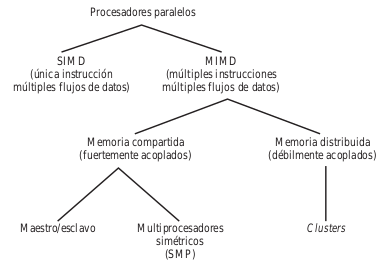
\includegraphics[width=0.8\textwidth, scale=1]{figura28.png}
				\end{figure}
				
				En un \textbf{multiprocesador simétrico (\textit{Symmetric Multiprocessor, SMP)}}, el núcleo puede ejecutar en cualquier procesador, y normalmente cada procesador realiza su propia planificación del conjunto disponible de procesos e hilos. El núcleo puede construirse como múltiples procesos o múltiples hilos, permitiéndose la ejecución de partes del núcleo en paralelo. El enfoque SMP complica el sistema operativo, ya que debe asegurar que dos procesadores no seleccionan un mismo proceso y que no se pierde ningún proceso de la cola. Se deben emplear técnicas para resolver y sincronizar el uso de los recursos.
				
				
	\section{Descripción y control de procesos}
		El diseño de un SO debe reflejar ciertos requisitos generales. Todos los SOs multiprogramados que son capaces de dar soporte a miles de usuarios, se construyen en torno al concepto de proceso. La mayoría de los requisitos que un SO debe cumplir se pueden expresar con referencia a los procesos: 
		
		\begin{itemize}
		\item El SO debe intercalar la ejecución de múltiples procesos, para maximiar la utilización del procesador mientras se proporciona un tiempo de respuesta razonable.
		\item El sistema operativo debe reservar recursos para los procesos conforme a una política específica (por ejemplo, ciertas funciones o aplicaciones son de mayor prioridad) mientras que al mismo tiempo evita interbloqueos.
		\item Un sistema operativo puede requerir dar soporte a la comunicación entre procesos y la creación de procesos, mediante las cuales ayuda a la estructuración de las aplicaciones.
		\end{itemize}
		
		\subsection{¿Qué es un proceso?}
			\subsubsection{Procesos y bloques de control de procesos}
				También se puede pensar en un proceso como en una entidad que consiste en un número de elementos. Los dos elementos esenciales serían el \textbf{código de programa} (que puede compartirse con
otros procesos que estén ejecutando el mismo programa) y un \textbf{conjunto de datos} asociados a dicho código.
				
				En cualquier instante puntual del tiempo, mientras el proceso está en ejecución, un proceso se puede caracterizar por una serie de elementos que incluyen:
				
				\begin{itemize}
				\item \textbf{Indentificador.} Un identificador único asociado a este proceso, para distinguirlo del resto de procesos.
				\item \textbf{Estado.} Si el proceso está actualmente corriendo, está en el estado en ejecución.
				\item \textbf{Prioridad.} Nivel de prioridad relativo al resto de procesos.
				\item \textbf{Contador de programa.} La dirección de la siguiente instrucción del programa que se ejecutará.
				\item \textbf{Punteros a memoria.} Incluye los punteros al código de programa y los datos asociados a dicho proceso, además de cualquier bloque de memoria compartido con otros procesos.
				\item \textbf{Datos de contexto.} Estos son datos que están presentes en los registros del procesador cuando el proceso está corriendo.
				\item \textbf{Información de estado de E/S.} Incluye las peticiones de E/S pendientes, dispositivos de E/S asignados a dicho proceso, una lista de los ficheros en uso por el mismo, etc.
				\item \textbf{Información de auditoría.} Puede incluir la cantidad de tiempo de procesador y de tiempo de reloj utilizados, así como los límites de tiempo, registros contables, etc.
				\end{itemize}
				
				La información de la lista anterior se almacena en una estructura de datos, que se suele llamar bloque de control de proceso (\textit{process control block (PCB)})(\ref{figura2.1:pcb}), que el SO crea y gestiona. El punto más significativo del PCB es que contiene suficiente información de forma que es posible interrumpir el proceso cuando está corriendo y posteriormente restaurar su estado de ejecución como si no hubiera habido interrupción alguna. Es la herramienta clave que permite al sistema operativo dar soporte a múltiples procesos y proporcionar multiprogramación. Cuando un proceso se interrumpe, los valores actuales del contador de programa y los registros del procesador (datos de contexto) se guardan en los campos correspondientes del BCP y el estado del proceso se cambia a cualquier otro valor, como bloqueado o listo. El sistema operativo es libre ahora para poner otro proceso en estado de ejecución. El contador de programa y los datos de contexto se recuperan y cargan en los registros del
procesador y este proceso comienza a correr. \\
				
				\begin{figure}
				\caption{PCB simplificado}
				\label{figura2.1:pcb}
				\centering
				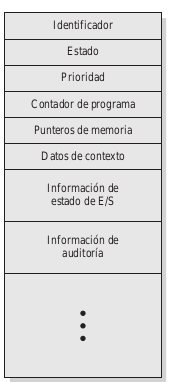
\includegraphics[width=0.4\textwidth, scale=1]{tema_2_figura1.png}
				\end{figure}
				
				De esta forma se puede decir que un proceso está compuesto por el código de programa y los datos asociados, además del PCB.
				
		\subsection{Estado de los procesos}
			Para que un programa se ejecute se necesita crear un proceso o tarea para dicho programa. Desde el punto de vista del procesador, el ejecuta instrucciones de su repertorio de instrucciones en una secuencia dictada por el cambio de los valores del registro contador de programa. A lo largo del tiempo, el contador de programa puede apuntar al código de diferentes porgramas que son parte de diferentes procesos. Desde el punto de vista de un programa individual, su ejecución
implica una secuencia de instrucciones dentro de dicho programa. \\
			
			Se puede caracterizar el comportamiento de un determinado proceso, listando la secuencia de instrucciones que se ejecutan para dicho proceso. A esta lista se la denomina traza del proceso. Se puede caracterizar el comportamiento de un procesador mostrando cómo las trazas de varios procesos se entrelazan. \\
			
			De manera adicional, existe un pequeño programa \textbf{activador}(\textit{dispatcher}) que intercambia el procesador de un proceso a otro. Hay que tener en cuenta cuando se vea la traza desde el punto de vista del procesador que para intercambiar el procesador entre procesos el dispatcher debe ejecutar una serie de instrucciones y que estas se deben tener en cuenta en la traza. Luego si se ejecuta un proceso y este finaliza o se expulsa (por ejemplo por temporarización) se llama al dispatcher que ejecuta una serie de instrucciones y luego se inicia el siguiente proceso a ejecutar. Luego la traza desde el punto de vista del procesador serían las instrucciones ejecutadas por el proceso más las ejecutadas por el dispatcher para interacmbiar el proceso.
			
			\subsubsection{Modelo de dos estados}
				La responsabilidad principal del sistema operativo es controlar la ejecución de los procesos; esto incluye determinar el patrón de entrelazado para la ejecución y asignar recursos a los procesos. El primer paso en el diseño de un sistema operativo para el control de procesos es describir el comportamiento que se desea que tengan los procesos. \\
				
				Se puede construir el modelo más simple posible observando que, en un instante dado, un proceso está siendo ejecutando por el procesador o no. En este modelo, un proceso puede estar en dos estados: Ejecutando o No Ejecutando. Cuando el sistema operativo
crea un nuevo proceso, crea el bloque de control de proceso (BCP) para el nuevo proceso e inserta dicho proceso en el sistema en estado No Ejecutando. El proceso existe, es conocido por el sistema
operativo, y está esperando su oportunidad de ejecutar. De cuando en cuando, el proceso actualmente
en ejecución se interrumpirá y una parte del sistema operativo, el activador (notese que el dispatcher forma parte del SO), seleccionará otro proceso a ejecutar. El proceso saliente pasará del estado Ejecutando a No Ejecutando y pasará a Ejecutando un nuevo proceso. \\
				
				Cada proceso debe representarse de manera que el SO pueda seguirle la pista, debe haber información correspondiente a cada proceso tal como el estado actual y su localización de memoria (PCB). Los procesos que no están ejecutando deben estar en una especie de cola, esperando su turno de ejecución. Existe una cola cuyas entradas son puntero al PCB de un proceso particular. Alternativamente, la cola debe consistir en una lista enlazada de bloques de datos, en la cual cada bloque representa un proceso. \\
				
				Un proceso que se interrumpe se transfiera a la cola de procesos en espera. Alternativamente, si el proceso ha finalizado o se aborta, se descarta (sale del sistema), y en ambos caso el dispatcher selecciona un nuevo proceso de la cola para ejecutar.
				
			\subsubsection{Creción y terminación de procesos}
				\textbf{Creación de un proceso.} Cuando se va a añadir un nuevo proceso a aquellos que se están gestionando en un determinado momento, el sistema operativo construye las estructuras de datos que
se usan para manejar el proceso (PCB) y reserva el espacio de direcciones en memoria principal para el proceso. Estas acciones constituyen la creación de un nuevo
proceso.
				\begin{figure}
				\caption{Razones para la creación de un proceso}
				\label{figura2.2:creacionprocesos}
				\centering
				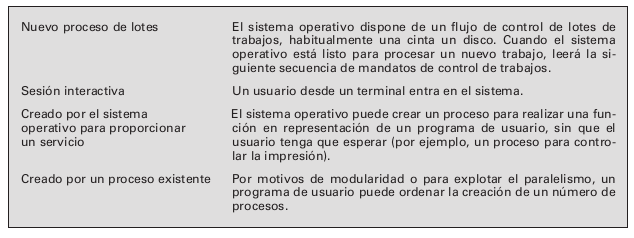
\includegraphics[width=1.1\textwidth, scale=1]{tema_2_figura2.png}
				\end{figure}
				
				En la figura \ref{figura2.2:creacionprocesos} se muestran las razones de creación de un proceso.
				
				Tradicionalmente, un SO creaba todos los procesos de forma transparente para usuarios y programas. Sin embargo, puede ser muy útil permitir a un proceso la creación de otro. Cuando un SO crea un proceso a petición explícita de otro proceso, dicha acción se denomina creación del proceso. \\
				
				Cuando un proceso lanza a otro, al primero se le denomina \textbf{proceso padre}, y al creado \textbf{proceso hijo}. La realación entre procesos suele necesitar comunicación y cooperación entre ellos.
				
				\textbf{Terminación de procesos}. En la figura \ref{figura2.3:terminaciónprocesos} se muestran las razones típicas para la terminación de un proceso. Todo sistema debe proporcionar los mecanismo mediante los cuales un proceso indica su finalicazión. Todas las acciones de finalización conllevan la solicitud de un servicio al sistema operativo para terminar con el proceso solicitante.
				
				\begin{figure}
				\caption{Razones para la terminación de un proceso.}
				\label{figura2.3:terminaciónprocesos}
				\centering
				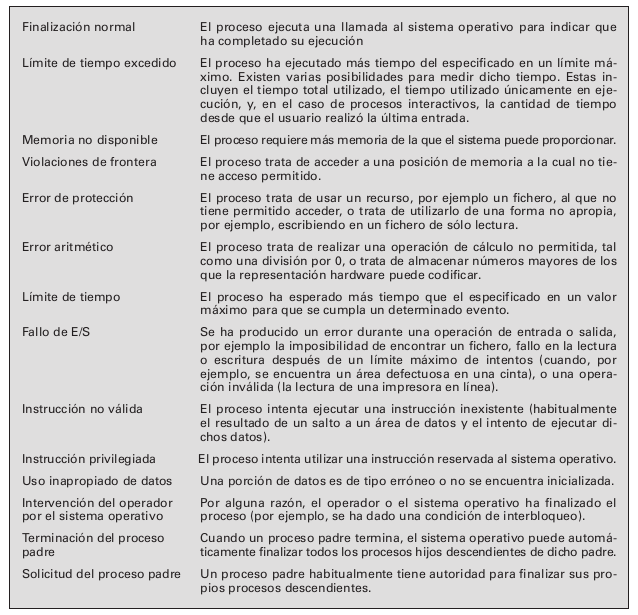
\includegraphics[width=1.2\textwidth, scale=1]{tema_2_figura3.png}
				\end{figure}	
				
				Adicionalmente, un número de error o una condición de fallo puede llevar a la finalización de un proceso. \\
				
			\subsubsection{Modelo de proceso de cinco estados}
				La cola es una lista de tipo FIFO y el procesador opera siguiendo una
estrategia cíclica (round-robin o turno rotatorio) sobre todos los procesos disponibles (cada proceso
de la cola tiene cierta cantidad de tiempo, por turnos, para ejecutar y regresar de nuevo a la cola, a
menos que se bloquee).	 \\

				En contraposición al modelo de dos estados, una forma más natural es dividir el estado No ejecutando en dos estados, listo y bloqueado. Para gestionarlo correctamente, se han añadido dos estados adicionales que resultarán muy útiles. 
				
				\begin{figure}
				\caption{Modelo de proceso de cinco estados}
				\label{figura2.4:cinco estados}
				\centering
				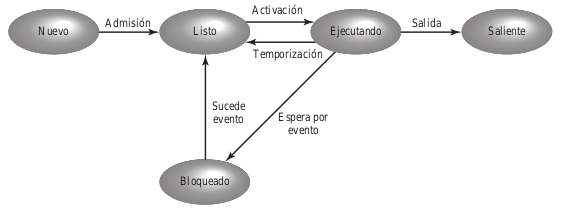
\includegraphics[width=0.8\textwidth, scale=1]{tema_2_figura4.png}
				\end{figure}
				
				Los cinco estados disponibles de un proceso son: 
				\begin{itemize}
				\item \textbf{Ejecutando.} El proceso está actualmente en ejecución.
				\item \textbf{Listo.} Un proceso que se prepara para ejecutar cuando tenga oportunidad.
				\item \textbf{Bloqueado.} Un proceso que no puede ejecutar hasta que se cumpla un evento determinado o
se complete una operación E/S.
				\item \textbf{Nuevo.} Un proceso que se acaba de crear y que aún no ha sido admitido en el grupo de procesos ejecutables por el sistema operativo. Típicamente, se trata de un nuevo proceso que no ha
sido cargado en memoria principal, aunque su bloque de control de proceso (BCP) si ha sido creado.
				\item \textbf{Saliente.} Un proceso que ha sido liberado del grupo de procesos ejecutables por el sistema operativo, debido a que ha sido detenido o que ha sido abortado por alguna razón.
				\end{itemize}
									
				Los estados Nuevo y Saliente son útiles para construir la gestión de procesos. Si se solicita un nuevo trabajo a un sistema de procesamiento por lotes, el SO puede definir un nuevo proceso en dos etapas. Primero, el SO realiza todas las tareas internas que correspondan. Se asocia un identificador al proceso. Se reservan y construyen todas las tables para gestionar el proceso. En este punto, el proceso estará en estado Nuevo. Mientras un proceso está en el estado nuevo, la información realitva al proceso que se necesite por parte del SO se mantiene en tablas de control de memoria principal. Sin embargo, el proceso en sí mismo no se encuentra en memoria principal. Esto es, el código de programa a ejecutar no se encuentra en meoria principal, y no se ha reservado ningún espacio para los datos asociados al programa. \\
				
				De forma similar, un proceso sale del sistema en dos fases. Primero, el proceso termina cuando alcanza su punto de finalización natural, cuando es abortado debido a un error irrecuperable, o cuando otro proceso con mayor autoridad causa que el proceso se aborte. La terminación mueve el proceso a Saliente. En este punto, el proceso no es elegible de nuevo para su ejecución. Las tablas y otra información asociada con el trabajo se encuentran temporalmente preservadas por el sistema operativo, el cual proporciona tiempo para que programas auxiliares o de soporte extraigan la información necesaria (programas de utilidad, auditoría, etc.). Una vez que estos programas han extraído la información necesario, el SO no necesita mantener ningún dato relativo al proceso y el proceso se borra del sistema.
				
				Las posibles transacciones de estado de un proceso son las siguientes:
				
				\begin{itemize}
				\item \textbf{Null $\rightarrow$ Nuevo}. Se crea un nuevo proceso para ejecutar un programa. (\ref{figura2.2:creacionprocesos}).
				\item \textbf{Nuevo $\rightarrow$ Listo.} El SO mueve a un proceso del estado nuevo a listo cuando éste se encentre preparado para ejecutar un nuevo proceso. Las
tablas y otra información asociada con el trabajo se encuentran temporalmente preservadas por el sistema operativo, el cual proporciona tiempo para que programas auxiliares o de soporte extraigan la información necesaria.
				\item \textbf{Listo $\rightarrow$ Ejecutando.} Cuando llega el momento de seleccionar un nuevo proceso para ejecutar, el SO selecciona uno de los procesos en estado listo. Esta es una tarea que lleva a cabo el planificador.
				\item \textbf{Ejecutando $\rightarrow$ Saliente.} El proceso actual en ejecución se finaliza por parte del SO tanto si el proceso indica que ha completado su ejecución como si éste aborta.
				\item \textbf{Ejecutando $\rightarrow$ Listo.} La razón más habitual para esta transición es que el proceso en ejecución haya alcanzado el máximo tiempo posible de ejecución de forma ininterrumpida;
prácticamente todos los sistemas operativos multiprogramados imponen este tipo de restric-
ción de tiempo. Es de particular importancia el caso en el cual el sistema operativo asigna diferentes niveles de prioridad a diferentes procesos. Si un proceso de más prioridad está bloqueado a las espera de una condición y se produce esta condición, este pasará al estado de listo y se puede dar que expulse del procesador al proceso que se esté ejecutando si este tiene una menor prioridad.
				\item \textbf{Ejecutando $\rightarrow$ Bloqueado.} Un proceso se pone en el estado Bloqueado si solicita algo por lo cual debe esperar. Una solicitud al sistema operativo se realiza habitualmente por medio de
una llamada al sistema; esto es, una llamada del proceso en ejecución a un procedimiento que es parte del código del sistema operativo.
				\item \textbf{Bloqueado $\rightarrow$ Listo.} Un proceso en estado bloqueado se mueve al estado listo cuando sucede el evento por el cual estaba esperando.
				\item \textbf{Listo $\rightarrow$ Saliente.} En algunos sistemas, un padre puede terminar la ejecución de un proceso hijo en cualquier momento. También, si el padre termina, todos los procesos hijos asociados con dicho padre pueden finalizarse.
				\item \textbf{Bloqueado $\rightarrow$ Saliente.} Se aplican los comentarios del caso anterior.
				
				\item En general, el término expulsión (\textbf{\textit{preemption}}) se define como la reclamación de un recurso por parte de un proceso antes de que el proceso que lo poseía finalice su uso. En este caso, el recurso es el procesador.
				\end{itemize}
				
				Se pueden sugerir una forma de aplicar dos colas: la de listos y la de bloqueados. Cada proceso admitido por el sistema, se coloca en la cola de los listos. Cuando llega el momento de que el SO seleccione otro proceso a ejecutar, selecciona uno de la cola de listos. En ausencia de priorida, esta cola puede ser una lista de tipo FIFO. Cuando el proceso en ejecución termina de utilizar el procesador, o bien finaliza o bien se coloca en la cola de listos o de bloqueados, dependiendo de las circunstancias. Por úlitmo, cuando sucede un evento, cualquier proceso en la cola de bloqueados que únicamente esté esperando dicho evento, se mueve a listos.
				
				En los SOs con muchos procesos, si varios procesos esperan por un mismo evento al producirse el mismo todos los procesos de la cola de bloqueados que pertenezcan a la cola de dicho evento se enviarán a listo. \\
				Si la activación de procesos está dictada por un esquema de prioridades, sería conveniente tener varias colas de procesos listos, una por cada nivel de prioridad. El sistema operativo podría determinar cual es el proceso listo de mayor prioridad simplemente seleccionando éstas en orden.
			\subsubsection{Procesos suspendidos}
				\textbf{La necesidad de intercambio o swapping}.Existe una buena justificación para añadir otros estados al modelo. Cada proceso que se ejecuta debe cargarse completamente en memoria principal. Se podría dar el caso en el que debido a que la diferencia de velocidad entre procesador y E/S es tal que todos los procesos en memoria se podrían encontrar bloqueados a la espera de dichas oepraciones. Por tanto, incluso en un sistema multiprogramado, el procesador puede estar ocioso la mayor parte del tiempo. \\
				
				La memoria principal puede expandirse para acomodar más procesos. Hay dos fallos en esta solución. Primero, existe un coste asociado a la memoria principal, que, desde un coste reducido a nivel de bytes, comienza a incrementarse según nos acercamos a un almacenamiento de gigabytes. Segundo, el apetito de los programas a nivel de memoria ha crecido tan rápido como ha bajado el coste de las memorias. De forma que las grandes memorias actuales han llevado a ejecutar procesos de gran tamaño, no más procesos. \\
				
				Otra solución es el \textit{swapping}(memoria de interacmbio), que implica mover parte o todo el proceso de memoria principal al disco. Cuando ninguno de los procesos en memoria principal se encuentra en estado Listo, el sistema operativo intercambia uno de los procesos bloqueados a disco, en la cola de Suspendidos. Esta es una lista de procesos existentes que han sido temporalmente expulsados de la memoria principal, o suspendidos. El SO trae otro proceso de la cola de Suspendidos o responde a una solicitud de un nuevo proceso, de forma que la ejecución continúa con los nuevos procesos. \\
				
				El \textit{swapping}, sin embargo, es una operación de E/S, y por tanto existe el riesgo potencial de hacer que el problema empeore. Pero debido a que la E/S en disco es habitualmente más rápida que la E/S sobre otros sistemas, el \textit{swapping} suele mejorar el rendimiento del sistema. \\
				
				Con el uso de swapping tal y como se ha escrito, debe añadirse un nuevo estado a nuestro modelo de comportamiento, el estado suspendido. Cuando todos los procesos en memoria principal se encuentran en estado Bloqueado, el sistema operativo puede suspender un proceso poniéndolo en el estado Suspendido y transfiriéndolo a disco. El espacio que se libera en memoria principal puede usarse para traer a otro proceso. \\
				
				Cuando el sistema operativo ha realizado la operación de swap (transferencia a disco de un proceso), tiene dos opciones para seleccionar un nuevo proceso para traerlo a memoria principal: puede admitir un nuevo proceso que se haya creado o puede traer un proceso que anteriormente se encontrase en estado de Suspendido. Parece que sería preferible traer un proceso que anteriormente estuviese suspendido, para proporcionar dicho servicio en lugar de incrementar la carga total del
sistema. \\
				
				Este razonamiento tiene una dificulta, que todos los procesos que se suspendieron estaban previamente bloqueados. Claramente no sería bueno traer un proceso bloqueado de nuevo a memoria porque podría no encontrarse todavía listo para la ejecución. Se debe reconocer que todos los procesos en estado bloqueado están a la espera del suceso de un evento, luego cuando ese evento ocurre pasa a estar listo. \\
				
				Para el nuevo modelo se requieren de cuatro estados: 
				\begin{itemize}
				\item \textbf{Listo.} El proceso está disponible para ejecución.
				\item \textbf{Bloqueado.} El proceso esta en memoria principal a la espera de un proceso.
				\item \textbf{Bloqueado/Suspendido.} El proceso está en almacenamiento secundario y esperando un evneto.
				\item \textbf{Listo/Suspendido.} El proceso está en almacenamiento secundario pero disponible para ejecución tan pronto se cargue en memoria principal.
				\end{itemize}
				
				La explicación ha asumido que no se utiliza memoria virtual y que un proceso está completamente en memoria principal, o completamente fuera de la misma. Con
un esquema de memoria virtual, es posible ejecutar un proceso que está sólo parcialmente en memoria principal. Si se hace referencia a una dirección de proceso que no se encuentra en memoria principal, la porción correspondiente del proceso se trae a ella. El uso de la memoria principal podría parecer que elimina la necesidad del swapping explícito, porque cualquier dirección necesitada por un
proceso que la demande puede traerse o transferirse de disco a memoria por el propio hardware de gestión de memoria del procesador. Sin embargo, el rendimiento de los sistemas de memoria virtual pueden colapsarse si hay un número de suficientemente grande de procesos activos, todos ellos están parcialmente en memoria principal. De esta forma, incluso con un sistema de memoria virtual, el sistema operativo necesita hacer swapping de los procesos de forma explícita y completa, de vez en cuando, con la intención de mejorar el rendimiento. \\
				
				\begin{figure}
				\caption{Diagrama de transición de estados de procesos con dos estados suspendidos.}
				\label{figura2.5:estadossuspendidos}
				\centering
				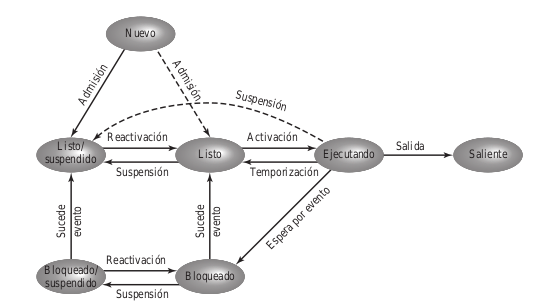
\includegraphics[width=0.8\textwidth, scale=1]{tema_2_figura5.png}
				\end{figure}
				
				Veamos las nuevas transiciones más importantes:
				
				\begin{itemize}
				\item \textbf{Bloqueado $\rightarrow$ Bloqueado/Suspendido.} Si no hay procesos listos, entonces al menos uno de los procesos bloqueados se transfiere al disco para hacer espacio para otro proceso que no se encuentra bloqueado. Esta transición se puede realizar incluso si hay procesos listos, si el SO determina que el proceso actualmente en ejecución o los procesos listos requieren más memoria principal para mantener un rendimiento adecuado.
				\item \textbf{Bloqueado/Suspendido $\rightarrow$ Listo/Suspendido.} Un proceso en el estado Bloqueado/Suspendido se mueve al estado Listo/Suspendido cuando sucede un evento al que estaba esperando. Nótese que esto requiere que la información de estado concerniente a un proceso suspendido sea accesible para el sistema operativo.
				\item \textbf{Listo/Suspendido $\rightarrow$ Listo.} Cuando no hay más procesos listos en memoria principal, el sistema operativo necesitará traer uno para continuar la ejecución. Adicionalmente, puede darse el caso de que un proceso en estado Listo/Suspendido tenga mayor prioridad que cualquiera de los procesos en estado Listo. En este caso, el sistema operativo puede haberse diseñado para determinar que es más importante traer un proceso de mayor prioridad que para minimizar el efecto del swapping.
				\item \textbf{Listo $\rightarrow$ Listo/Suspendido.} Puede ser necesario suspender un proceso Listo si con ello se consigue liberar un bloque suficientemente grande de memoria. También el sistema operativo puede decidir suspender un proceso Listo de baja prioridad antes que un proceso Bloqueado de alta prioridad, si se cree que el proceso Bloqueado estará pronto listo. \\
				
				Otras transiciones interesantes son:
				
				\item \textbf{Nuevo $\rightarrow$ Listo/Suspendido y Nuevo a Listo.} Cuando se crea un proceso nuevo, puede añadirse a la cola de Listos o a la cola de Listos/Suspendidos. En cualquier caso, el sistema operativo puede crear un bloque de control de proceso (BCP) y reservar el espacio de direcciones del proceso. Puede ser preferible que el sistema operativo realice estas tareas internas cuanto antes, de forma que pueda disponer de suficiente cantidad de procesos no bloqueados. Sin embargo, con esta estrategia, puede ocurrir que no haya espacio suficiente en memoria principal para el nuevo proceso; de ahí el uso de la transición (Nuevo $\rightarrow$ Listo/Suspendido). Por otro lado haciendo la creación de procesos cuanto más tarde, se hace posible reducir la sobrecarga del SO y le permite realizar las tareas de creación de procesos cuando el sistema está lleno de procesos bloqueados.
				\item \textbf{Bloqueado/Suspendido $\rightarrow$ Bloqueado.} Un proceso termina, liberando alguna memoria principal. Hay un proceso en la
cola de Bloqueados/Suspendidos con mayor prioridad que todos los procesos en la cola de Listos/Suspendidos y el sistema operativo tiene motivos para creer que el evento que lo bloquea va a ocurrir en breve. Bajo estas circunstancias, sería razonable traer el proceso Bloqueado a memoria por delante de los procesos Listos.
				\item \textbf{Ejecutando $\rightarrow$ Listo/Suspendido.} Si un proceso está ejecutando pero un proceso de mayor prioridad que estaba en la cola de Bloqueado/Suspendido se desbloquea, el SO puede producir una preemption y enviar el proceso que se estaba ejecutando directamente a la cola de Listo/Suspendido para así liberar memoria para el proceso de mayor prioridad.
				
				\item \textbf{De cualquier estado $\rightarrow$ Saliente.} Habitualmente, un proceso termina cuando está ejecutando, bien porque ha completado su ejecución o debido a una condición de fallo. Sin embargo, en algunos sistemas operativos un proceso puede terminarse por el proceso que lo creó o cuando el proceso padre a su vez ha terminado. Si se permite esto, un proceso en cualquier estado puede moverse al estado Saliente.			
				\end{itemize}
				
				\textbf{Otros usos para la suspensión de procesos.} Podemos analizar el concepto de proceso suspendido, definiendo un proceso suspendido como el que cumple las siguientes características:
				
				\begin{enumerate}
				\item El proceso no está inmediatamente disponible para su ejecución.
				\item El proceso puede estar o no a la espera de un evento, si es así, la condición de bloqueo es independiente de la condición estar suspendido, y si sucede el evento que lo bloquea, eso no habilita al proceso para su ejecución inmediata.
				\item El proceso fue puesto en estado suspendido por un agente: bien el proceso mismo, el proceso padre o el sistema operativo, con el propósito de prevenir su ejecución.
				\item El proceso no puede ser recuperado de este estado hasta que el agente explícitamente así lo indique.
				\end{enumerate}
				
				\begin{figure}
				\caption{Razones de suspensión de un proceso}
				\label{figura2.6:suspensión}
				\centering
				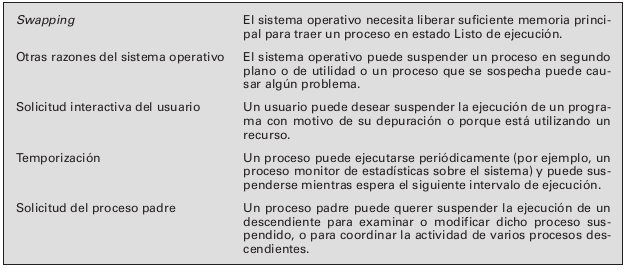
\includegraphics[width=1\textwidth, scale=1]{tema_2_figura6.png}
				\end{figure}
				
		\subsection{Descripción de procesos}
			El SO controla los eventos dentro del computador, planifica y activa los procesos para su ejecución por el procesador, reserva recursos para los mismos y responde a las solicitudes de servicios básicos de los procesos de usuarios. Fundamentalmente, se piensa en el SO como en la entidad que gestiona el uso de recursos del sistema por parte de los procesos. \\
			
			\begin{figure}
			\caption{Procesos y recursos(reserva de recursos instantánea del sistema}
			\label{figura2.7:procesosyrecurso}
			\centering
			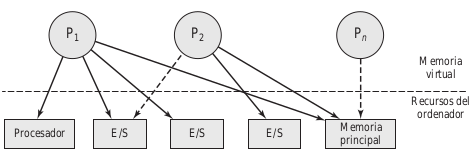
\includegraphics[width=0.8\textwidth, scale=1]{tema_2_figura7.png}
			\end{figure}
			
			En la figura \ref{figura2.7:procesosyrecurso} se observa este concepto. En un entorno multiprogramado, hay numerosos procesos (P1,... Pn) creados y residentes en memoria virtual. Cada proceso, durante el transcurso de su ejecución, necesita acceder a ciertos recursos del sistema, incluido el procesador, los dispositivos de E/S y la memoria principal. Enn la figura, P1 está ejecutando; al menos parte del proceso está en memoria principal, y controla dos dispositivos de E/S. P2 está también totalmente en memoria principal pero está bloqueado a la espera de un dispositivo de E/S asignado a P1. El proceso Pn se encuentra transferido a disco y está por tanto suspendido.
			
			\subsubsection{Estructuras de control del SO}
				Si el sistema operativo se encarga de la gestión de procesos y recursos, debe disponer de información sobre el estado actual de cada proceso y cada recurso. El mecanismo universal para proporcionar esta información es el siguiente: el sistema operativo construye y mantiene tablas de información sobre cada entidad que gestiona. A pesar de que los detalles difieren entre SOs todos mantienen información de memoria, E/S, ficheros y procesos.
				
				\begin{figure}
				\caption{Estructura general de las tablas de control del SO}
				\label{figura2.8:tablasdecontrol}
				\centering
				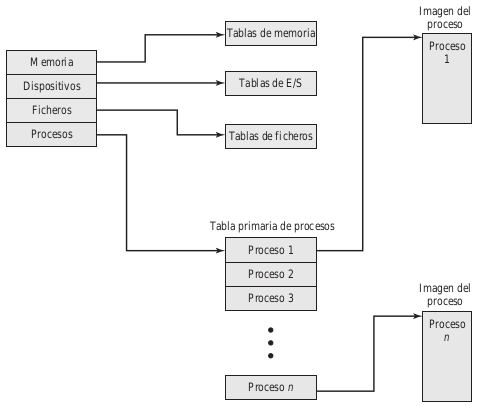
\includegraphics[width=0.8\textwidth, scale=1]{tema_2_figura8.png}
				\end{figure}
				
				Las \textbf{Tablas de memoria} se usan para mantener el registro tanto de la memoria principal (real) como de la secundaria (virtual). Parte de la memoria principal está reservada para el uso del SO;el resto está disponible para el uso de los procesos. Los procesos se mantienen en memoria secundaria utilizando algún tipo de memoria virtual o técnicas de swapping. Las tablas de memoria deben incluir la siguiente información:
				
				\begin{itemize}
				\item Las reservas de memoria principal por parte de los procesos.
				\item Las reservas de memoria secundaria por parte de los procesos.
				\item Todos los atributos de protección que restringe el uso de la memoria principal y virtual, de forma que los procesos puedan acceder a ciertas áreas de memoria compartida.
				\item La información necesaria para manejar la memoria virutal.
				\end{itemize}
				
				El SO debe utilizar las \textbf{tablas de E/S} para gesitonar los dispositivos de E/S y los canales del computador. Pero, en un instante determinado, un dispositivo E/S puede estar disponible o asignado a un proceso en particular. Si la operación de E/S se está realizando, el sistema operativo necesita conocer el estado de la operación y la dirección de memoria principal del área usada como fuente o destino de la transferencia de E/S. \\
				
				El SO también puede mantener las \textbf{tablas de ficheros}. Estas proporcionan información sobre las existencia de memoria, su posición en almacenamiento secundario, su estado actual, y otros atributos. La mayoría de, o prácticamente toda, esta información se puede gestionar por el sistema de ficheros, en cuyo caso el sistema operativo tiene poco o ningún conocimiento sobre los ficheros. \\
				
				El SO debe mantener \textbf{tablas de procesos} para gestionar los procesos. Las tablas anteriormente mencionadas se encuentran entrelazadas y referenciadas entre sí de alguna manera. Memoria, E/S, y ficheros se gestionan por parte de los procesos, de forma que debe haber algunas referencias en estos recursos, directa o indirectamente, desde las tablas de procesos. Los ficheros indicados en las tablas de ficheros son accesibles mediante dispositivos E/S y estarán, en algún caso, residentes en memoria virtual o principal. Las tablas son también accesibles para el sistema operativo, y además están controladas por la gestión de memoria.
				
			\subsubsection{Estructuras de control de procesos}
				Un SO para controlar y manejar procesos, primero, debe conocer dónde se localizan, y segundo, los atributos de aquellos que quiera gestionar (PID, estado \ldots). \\
				
				\textbf{Localización de procesos.} Como mínimo un proceso debe incluir un programa o conjunto de programas a ejecutar. Asociados a estos existen unas posiciones de emmoria para datos de variables locales y globales y de cualquier constante definida. Así, un proceso debe consistir en una cantidad suficiente de memoria para almacenar el programa y datos del mismo. Adicionalmente, la ejecución típica de un programa incluye una pila (\textit{véase} \pageref{Control de procedimientos})que se utiliza para las llamadas a procedimientos y los parámetros pasados entre dichos procedimientos. Por último, cada proceso está asociado a un número de atributos que son utilizados por el SO para controlar el proceso. Normalmente, el conjunto de estos atributos se llama \textbf{PCB}. Nos podemos referir al conjunto de \textbf{programa, datos, pila y atributos, como \textit{imagen del proceso}}. \\				
				
				\begin{figure}
				\caption{Elementos típicos de la imagen de un proceso.}
				\label{2.9:imagenproceso}
				\centering
				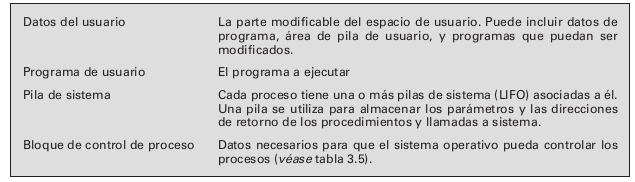
\includegraphics[width=0.9\textwidth, scale=1]{tema_2_figura9.png}
				\end{figure}
				
				La posición de la imagen del proceso dependerá del esquema de gestión de memoria que se utilice. En el caso más simple, la imagen del proceso se mantiene como un bloque de memoria contiguo, o continuo. Este bloque se mantiene en memoria secundaria. Para que el SO pueda gestionar el proceso, al menos una pequeña porción de su imagen se debe mantener en memoria principal. Para ejecutar el proceso, la imagen del proceso completa se debe cargar en memoria principal o al menos en memoria virtual. Asimismo, el sistema operativo necesita conocer la posición en disco de cada proceso y, para cada proceso que se encuentre en memoria principal, su posición en dicha memoria. Con \textit{Compatible Time-Sharing System}, cuando un proceso se transfiere a disco parte de la imagen del proceso permanece en memoria principal(no siempre ocurre). De esta forma, el SO debe mantener en registro qué partes de la imagen del proceso se encuentran todavía en memoria principal. \\
				
				Los sistemas operativos modernos suponen la existencia de un hardware de paginación que permite el uso de la memoria física no contigua, para dar soporte a procesos parcialmente residentes en la memoria principal. En esos casos, una parte de la imagen del proceso se puede encontrar en dicha
memoria principal, con las restantes en memoria secundaria. De esta forma, las tablas mantenidas por sistema operativo deben mostrar la localización de cada página de la imagen del proceso. En un sistema que utilice memoria virtual, toda imagen de un proceso activo se encuentra siempre en memoria secundaria. Sólo una parte de la imagen se carga en memoria principal, esta se copia no se mueve. De esta forma, la memoria secundaria mantiene una copia de todos los segmentos y/o páginas. Sin embargo, si la parte de imagen del proceso en memoria principal se ve modificada, la copia en memoria secundaria estará desactualizada hasta que la parte residente en memoria principall se copie de nuevo a disco. \\

				\textbf{Atributos de proceso.} Cualquier sistema operativo multiprogramado de la actualidad requiere una gran cantidad de información para manejar cada proceso. Como quedó explicado, esta información se puede considerar que reside en el bloque de control del proceso (BCP). Los diferentes sistemas organizarán esta información de formas diferentes. \\
				
				Podemos agrupar la información del PCB en tres categorías:
				\begin{itemize}
				\item Identificación del proceso.
				\item Información de estado del procesador.
				\item Información de control del proceso.
				\end{itemize}
				
				\begin{figure}
				\caption{Elementos típicos de un PCB}
				\label{figura2.10.12:PCB}
				\centering
				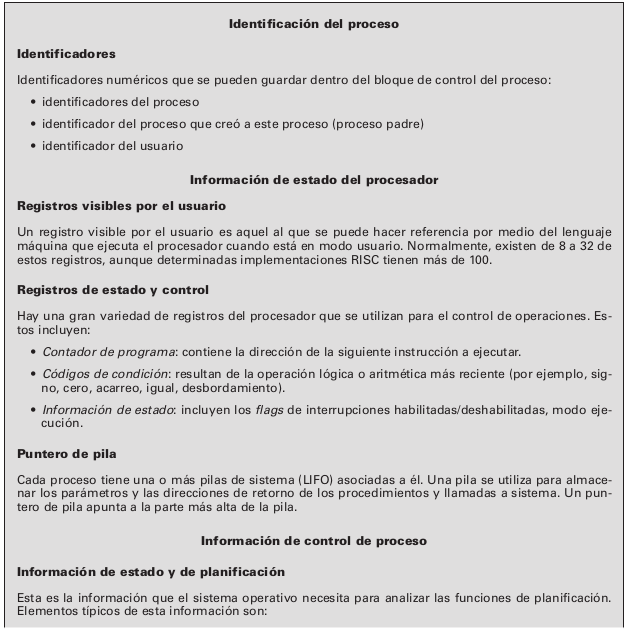
\includegraphics[width=0.9\textwidth, scale=1]{tema_2_figura10.png}
				\centering
				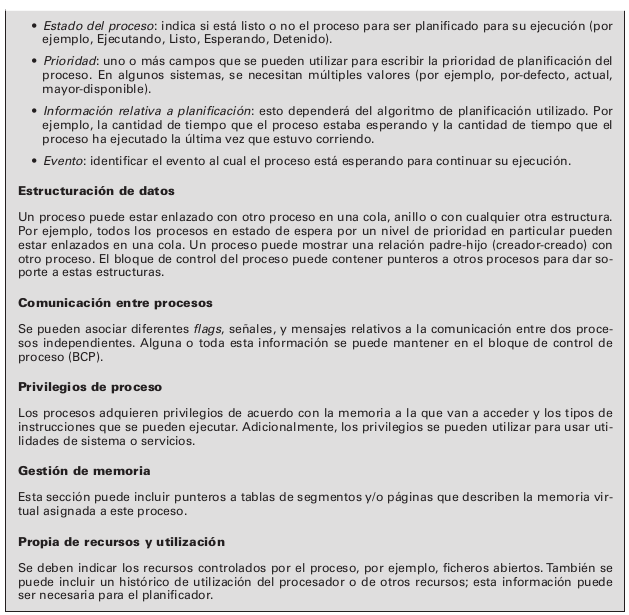
\includegraphics[width=0.9\textwidth, scale=1]{tema_2_figura11.png}
				\end{figure}
				
				Con respecto al \textbf{identificador de proceso}, en prácticamente todos los SOs, a cada proceso se le asocia un identificador numérico único, que puede ser simplemente un índice en la tabla de procesos principal; de otra forma, debe existir una traducción que permita al SO localizar las tablas apropiadas basándose en dicho identificador de proceso. Este identificador es útil para diferentes cuestiones. Muchas de las otras tablas controladas por el sistema operativo incluyen información que referencia a otro proceso por medio del identificador de proceso. Cuando un proceso se comunica con otro roceso informa al SO del destino de la comunicación. Cuando los procesos pueden crear otros procesos, los identificadores indican el proceso padre y los descendientes en cada caso.
				
				Junto con los PID, se pueden asignar UID que indica el usuario responsable del trabajo. \\
				
				La \textbf{información de estado de proceso} indica los contenidos de los registros del procesador.
Cuando un proceso está ejecutando, esta información está, por supuesto, en los registros. Cuando un proceso se interrumpe, toda la información de los registros debe salvaguardarse de forma que se pueda restaurar cuando el proceso continúe con su ejecución. La naturaleza y el número de estos registros depende del diseño del procesador. \\

				Se debe notar que, el diseño de todos los procesadores incluye un registro o conjuntos de registros, habitualmente conocidos como palabras de estado de programa (program status word, PSW) que contiene información de estado. La PSW típicamente contiene códigos de condición así como otra información de estado. \\
				
				\textbf{Inforamción de control de proceso.} Esta información adicional la necesita el SO para controla y coordinar varios procesos activos. \\
				
				\begin{figure}
				\caption{Registros EFLAGS de Pentium II (PSW)}
				\label{figura2.12:PSW_PENTIUM}
				\centering
				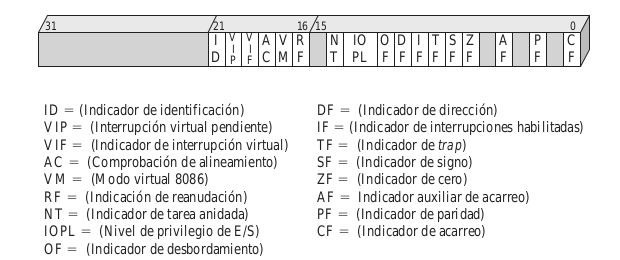
\includegraphics[width=1\textwidth, scale=1]{tema_2_figura12.png}
				\end{figure}
				
				\begin{figure}
				\caption{Procesos de usuario en memoria virtual}
				\label{figura2.13:procesos_mem_virtual}
				\centering
				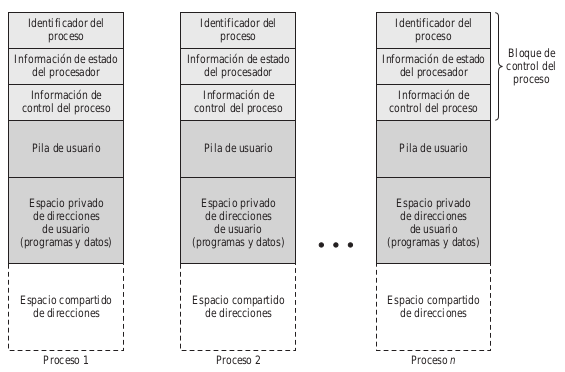
\includegraphics[width=1\textwidth, scale=1]{tema_2_figura13.png}
				\end{figure}
				
				La figura \ref{figura2.13:procesos_mem_virtual} sugiere la estructura de las imágenes de los procesos en memoria virtual. Cada imagen de proceso consiste en un PCB, y cualquier otro espacio de direcciones que el proceso comparta con otros procesos. En la figura, cada imagen de proceso aparece como un rango de direcciones contiguo, pero en una implementación real, no tiene por qué ser el caso; dependerá del esquema de gestión de memoria y de la forma en la cual se encuentren organizadas las estructuras de control por parte del SO. \\
				Un PCB puede contener información estructural, incluyendo puntero que permiten enlazar bloques de control de proceso entre sí. De esta forma, las colas que se describieron en la sección anterior pueden implementarse como listas enlazadas de PCB. \\
				
				\textbf{El papel del PCB.} El PCB es la más importante de las estructuras de datos del SO. Cada PCB contiene toda la información sobre un proceso que necesita el SO. Los bloques se leen y/o se modifican por la práctica totalidad de los módulos del SO, incluyendo aquellos relacionados con la planificación, la reserva de recursos, el procesamineto entre regiones, y el análisis y monitorización del rendimiento. Se puede decir que el conjunto de los bloques de control de proceso definen el estado del SO. \\
				
				Un gran número de rutinas dentro del SO necesitarán acceder a información de los PCB. Proporcionar acceso directo a estas tablas no es difícil. Cada proceso lleva asociado un único PID, que peude utilizarse para indexar dentro de una tabla de punteros a bloque de control de proceso. Dos posibles problemas serían:
				
				\begin{itemize}
				\item Un fallo en una simple rutina, como un manejador de interrupción, puede dañar los PCB, que puede destruir la capacidad del sistema para manejar los procesos afectados.
				\item Un cambio en la estructura o en la semántica de los PCB puede afectar a un gran número de módulos del SO.
				\end{itemize}
				
				Estos problemas se pueden ser tratar obligando a que todas rutinas del sistema operativo pasen a través de una rutina de manejador, cuyo único trabajo es proteger a los bloques de control de proceso, y que es la única que realiza el arbitraje en las operaciones de lectura y escritura de dichos bloques. Los factores a equilibrar en el uso de está rutina son, por un lado los aspectos de rendimiento, y por el otro, el grado en el cual el resto del software del sistema puede verificarse para determinar su corrección.
		\subsection{Control de proceso}
			\subsubsection{Modos de ejecución}
				Muchos procesadores proporcionan al menos dos modos de ejecución. Ciertas instrucciones se pueden ejecutar en modo privilegiado únicamente. Èstas incluirían lectura y modificación de registros de control(ej. PSW); instrucciones de E/S primitivas; e instrucciones relacionadas con la gestión de memoria. Adicionalmente, ciertas regiones de memoria sólo se pueden acceder en los modos más privilegiados. \\
				
				El modo menos privilegiado es el \textbf{modo usuario}, porque los programas de usuario típicamente se ejecutan en este modo. El más privilegiado es el \textbf{modo sistema, modo control o modo núcleo}. Este último se refiere al núcleo del SO, que es la parte del SO que engloba las funciones más importantes del sistema.  \\
				
				\begin{figure}
				\caption{Funciones típicas de un núcleo de SO}
				\label{figura2.14:funciones_kernel}
				\centering
				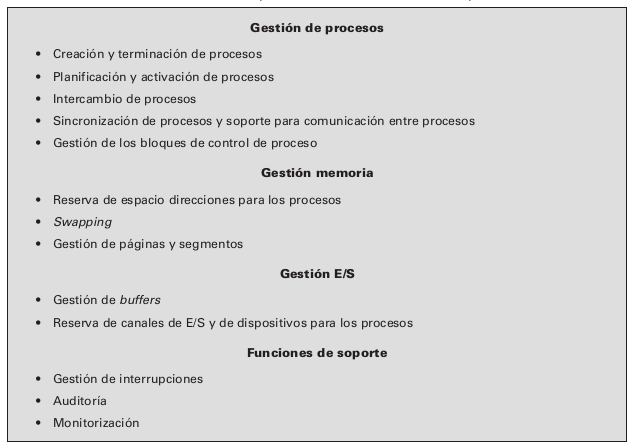
\includegraphics[width=1\textwidth, scale=1]{tema_2_figura14.png}
				\end{figure}
				
				Se necesita proteger al SO y a las tablas claves del sistema de la interferencia con programas de usuario. En modo núcleo, el software tiene control completo del procesador y de sus instrucciones, registros y memoria. Este nivel de control no es necesario y por seguridad tampoco es recomendable para los programas de usuario. \\
				
				Para que el procesador conozca el modo de ejecución, existe un bit en PSW que indica el modo de ejecución. Este cambia como respuesta a determinados eventos. Habitualmente, cuando un usuario realiza una llamada de servicio del SO o cuando una interrupción dispara la ejecución de una rutina del SO, este modo de ejecución se cambia a modo núcleo, y tras la finalización del servicio, se fija de nuevo el modo usuario. (cpl $\rightarrow$ \textit{current privilege level}, psr $\rightarrow$ registro de estado, en Intel Itanium).
				
			\subsubsection{Creación de procesos}
				Una vez que un SO decide crear un proceso procede de la siguiente manera:
				
				\begin{enumerate}
				\item \textbf{Asignar un identificador de proceso único al proceso.} En este instante, se añade una nueva entrada en la tabla primeria de procesos, que contiene un entrada por proceso.
				\item \textbf{Reserevar espacio para proceso.} Incluye todos los elementos de la imagen del proceso. Para ello, el SO debe conocer cuánta memoria se requiere para el espacio de direcciones privado (programas y datos) y la pila de usuario. Estos valores se pueden asignar por defecto en función del tipo de proceso, o pueden fijarse en base a la solicitud de creación de trabajo permitido por el usuario. Si un proceso es creado por otro, el padre puede pasar parámetros requeridos por el SO como parte de la solicitud de la creación de proceso. Si existe una parte del espacio de direcciones compartido por este nuevo proceso, se fijan los enlaces apropiados. Por último, se debe reservar espacio para el PCB.
				\item \textbf{Inicialización del PCB.} La parte de identificación de proceso del BCP contiene el identificador del proceso así como otros posibles identificadores, tal como el indicador del proceso padre. En la información de estado de proceso del BCP, habitualmente se inicializa con la mayoría de entradas a 0, excepto el contador de programa (fijado en el punto entrada del programa) y los punteros de pila de sistema (fijados para definir los límites de la pila del proceso). La parte de información de control de procesos se inicializa en base a los valores por omisión, considerando también los atributos que han sido solicitados para este proceso. Inicialmente, el proceso no debe poseer ningún recurso (dispositivos de E/S, ficheros) a menos que exista una indicación explícita de ello o que haya sido heredados del padre.
				\item \textbf{Establecer los enlaces apropiados.} Si el SO mantiene cada cola del planificador como una lista enlazada, el nuevo proceso debe situarse en la cola de Listos o en la cola de Listos/Suspendidos.
				\item \textbf{Creación o expansión de otras estructuras de datos.} El SO puede mantener un registro de auditoría por cada proceso que se puede utilizar posteriormente a efectos de facturación y/o de análisis de rendimiento del sistema.
				\end{enumerate}
				
			\subsubsection{Cambio de proceso}
				La operación de cambio de proceso puede parecer sencilla. En algunos casos, un proceso en ejecución se interrumpe para que el SO asigne a otro proceso el estado Ejecutando y de esta forma establece el turno entre los procesos. \\
				
				\textbf{Cuando se realiza el cambio de proceso.}     Puede ocurrir en cualuqier instante en el que el SO obtiene el control sobre el proceso actualmente en ejecución. \\
				
				\begin{figure}
				\caption{Mecanismos para la interrupción de la ejecución de un proceso}
				\label{figura2.15:interrupcion proceso}
				\centering
				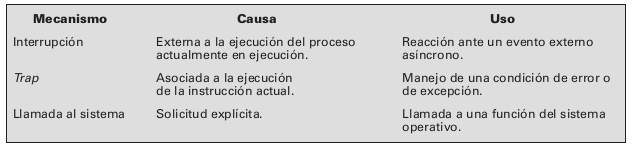
\includegraphics[width=1\textwidth, scale=1]{tema_2_figura15.png}
				\end{figure}
				
				Realmente podemos distinguir dos tipos de interrupciones de sistema, unas denominas interrupciones y otras denominadas \textit{traps}. Las primeras se producen por causa de algún tipo de evento que es externo e independiente del proceso actualmente en ejecución. Las otras asociadas a una condición de error o excepción generada dentro del proceso que está ejecutando, como un intento de acceso no permitido a un fichero. Dentro de una interrupción ordinaria, el control se transfiere al manejador de interrupción, que realiza determinadas tareas internas y salta a una rutina del SO. Ejemplos:
				\begin{itemize}
				\item \textbf{Interrupción de reloj.} El SO determina si el proceso en ejecución ha excedido o no la unidad máxima de tiempo de ejecución (\textit{time slice}). Esta es la máxima cantidad de timepo que un proceso puede ejecutar antes de ser interrumpido. En dicho caso, este proceso pasa al estado de listo y puede activar otro proceso.
				\item \textbf{Interrupción E/S.} El SO determina que acción de E/S ha ocurrido. Si uno o varios procesos esperan por esta acción, el SO mueve los procesos correspondientes al estado de listo( y los de estado bloqueado/supendido a listo/suspendido). El SO puede decidir si reanuda la ejecuciónd el proceso actualmente en estado ejecutando o si expulsa para proceder a la ejecución de un proceso de mayor prioridad.
				\item \textbf{Fallo de memoria}. El procesador se encuentra con una referencia a una dirección de memoria virtual, a una palabra que no se encuentra en memoria principal. El SO debe traer el bloque que contiene la referencia desde memoria secundaria a memoria principal. Después de que se solicita la operación de E/S para traer el bloque de memoria, el proceso que causó el fallo se pasa al estado bloqueado; el SO realiza un cambio de proceso y pone a ejecutar a otro proceso. Después de que el bloque e memoria se haya traído, el proceso pasará al estado Listo.
				\end{itemize}
				
				Con un \textbf{trap}, el SO conoce si una condición de error o de excepción es irreversible. Si es así, el proceso en ejecución se pone en el estado Saliente y se hace un cambio de proceso. De no ser así, el sistema operativo actuará dependiendo de la naturaleza del error y su propio diseño. Se puede intentar un procedimiento de recuperación o simplemente la notificación al usuario, pudiendo implicar tanto un cambio de proceso como la continuación de la ejecución del proceso actual. \\
				
				El SO se puede activar por medio de una llamada al sistema procedente del programa en ejecución. Esta llamada implica un salto a una rutina que es parte del código del SO. La realización de una llamada al sistema puede implicar en algunos casos que el proceso que la realiza pasa a Bloqueado. \\
				
				\textbf{Cambio de modo.} En la fase de interrupción, el procesador comprueba que no exista ninguna interrupción pendiente, indicada por la presencia de una señal de interrupción. Si no hay interrupciones pendientes, el procesador pasa a la fase de búsqueda de instrucción, siguiendo con el programa del proceso actual. Si hay interrupción pendiente, el proceso actúa de la siguiente manera:
				
				\begin{enumerate}
				\item Coloca el PC en la dirección de comienzo de la rutina del programa manejador de interrupción.
				\item Cambia de modo usuario a modo núcleo de forma que el código de tratamiento de interrupción pueda incluir instrucciones privilegiadas.
				\end{enumerate}

				El procesador, acto seguido, pasa a la fase de búsqueda de instrucción y busca la primera instrucción del programa de manejo de interrupción, que dará servicio a la misma. En este punto, habitualmente, el contexto del proceso que se ha interrumpido se salvaguarda en el bloque de control de proceso del programa interrumpido. \\
				
				Se debe salvaguardar toda la información que se pueda ver alterada por la ejecución de la rutina de interrupción y que se necesitará para la continuación del proceso interrumpido. De esta forma, se debe guardar la parte del PCB que hace referencia a la información de estado del procesador. Esto incluye PC, otros registros del procesador, y la información de la pila.	\\
				
				El manejador de interrupción es
habitualmente un pequeño programa que realiza unas pocas tareas básicas relativas a la interrupción. Por ejemplo, borra el flag o indicador que señala la presencia de interrupciones. Puede enviar una confirmación a la entidad que lanzó dicha interrupción, como por ejemplo el módulo de E/S. Y puede realizar algunas tareas internas variadas relativas a los efectos del evento que causó la interrupción. Si la interrupción proviene del reloj, el manejador de rutina le  pasará el control al \textit{dispatcher} que decidirá pasar a otro proceso pues el tiempo de procesador asignado a un proceso ha terminado. \\
				
				Si a esta interrupción le sigue un cambio de proceso a otro proceso, se necesitan más cosas. Sin embargo, en muchos SOs, la existencia de una interrupción no implica el cambio de proceso. Es posible, por tanto, que después de la ejecución de la rutina de interrupción, la ejecución se reanude con el mismo proceso. En esos casos sólo se necesita salvaguardar la información del estado del procesador cuando se produce la interrupción y restaurarla cuando se reanude la ejecución. Habitualmente, las operaciones de salvaguarda y recuperación se realizan por hardware. \\
				
				\textbf{Cambio del estado del proceso.} Esta claro, por tanto, que el cambio de modo es un concepto distinto al de cambio de proceso. Un cambio de modo puede ocurrir sin que cambie el estado de procesos actualmente ejecutando. En dicho caso, la salvaguarda del estado y su posterior restauración comportan sólo una ligera sobrecarga. Sin embargo, si el proceso actualmente en estado Ejecutando, se va a mover a cualquier otro estado (Listo, Bloqueado, etc.), entonces el sistema operativo debe realizar cambios sustanciales en su entorno. Los pasos que se realizan para un cambio de proceso completo son:
				
				\begin{enumerate}
				\item Salvar el estado del procesador, incluyendo PC y otros registros
				\item Actualizar el PCB que está actualmente en estado ejecutando. Esto incluye cambiar el estado del proceso a otro estado. También se acutalizan otros cambios importantes, inlcuyendo la razón por la cual el proceso deja de estar ejecutando y otra información de auditoría.
				\item Mover el PCB a la cola apropiada.
				\item Slección de nun nuevo proceso a ejecutar.
				\item Actualizar el PCB elegido. Esto incluye pasarlo a ejecutando.
				\item Actualizar las estructuras de datos de gestión de memoria. Esto se puede necesitar, dependiendo de cómo se haga la traducción de direcciones.
				\item Restaurar el estado del procesador al que tenía en el momento en el que el proceso seleccionado salió del estado Ejecutando por última ez, leyendo los valores anteriores de PC y registros.
				\end{enumerate}
				
				El cambio de proceso que implica un cambio de estado, requier un mayor esfuerzo que un cambio de modo.
				
			\subsubsection{Ejecución del SO}
				\textbf{Núcleo sin procesos.} Una visión tradicional, que es común a muchos SOs antiguos, es la ejecución del SO fuera de todo proceso. Con esta visión, cuando el proceso en ejecución se interrumpe o invoca una llamada al sistema, el contexto se guarda y el control pasa al núcleo. El SO tiene su propia región de memoria y su propia pila de sistema para controlar la llamada de procedimientos y sus retornos. El SO puede realizar todas las funciones que necesite y restaurar el contexto del proceso interrumpido, que hace que se retome la ejecución del proceso de usuario afectado. De forma alternativa, el SO puede realizar la salvaguarda del contexto y la activación de otro proceso diferente. Si esto ocurre o no depende de la causa de la interrupción y de las circunstancias puntales del momento. \\
				
				En cualquier caso, el punto clave en este caso es que el concepto de proceso se aplica aquí únicamente a los programas de usuario. El código del sistema operativo se ejecuta como una entidad independiente que requiere un modo privilegiado de ejecución. \\
				
				\textbf{Ejecución dentro de los procesos de usuario.} Una alternativa que es común en los sistemas operativos de máquinas pequeñas (PC, estaciones de trabajo) es ejecutar virtualmente todo el software de sistema operativo en el contexto de un proceso de usuario. Esta visión es tal que el sistema operativo se percibe como un conjunto de rutinas que el usuario invoca para realizar diferentes funciones, ejecutadas dentro del entorno del proceso de usuario. En un punto determinado, el SO maneja n imágenes de procesos. Cada imagen incluye áreas de programa, datos y pila para los programas del núcleo. \\
				
				\begin{figure}
				\caption{Relación entre el SO y los procesos de usuario}
				\label{figura2.16:relaciónSO-procesos}
				\centering
				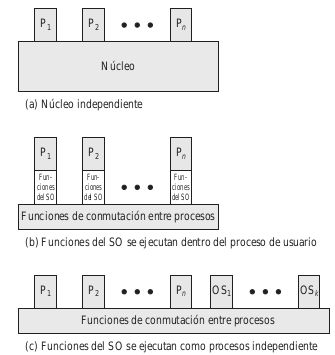
\includegraphics[width=0.8\textwidth, scale=1]{tema_2_figura16.png}
				\end{figure}
				
				Se sugiere la estrutura de imagen de proeso típica para esta estrategia. Se usa una pila de núcleo seperada para manejar llamadas/retornos cuando el proceso está en modo núcleo. El código del SO y sus datos están en el espacio de direcciones compartidas y se comparten entre todos los procesos.\\
				
				Cuando ocurre una interrupción, trap o llamada al sistema, el procesador se pone en modo núcleo y el control pasa al SO. Para este fin, el contexto se salva y se cambia de
modo a una rutina del sistema operativo. Sin embargo, la ejecución continúa dentro del proceso de usuario actual. De esta forma, no se realiza un cambio de proceso, sino un cambio de modo dentro del mismo proceso. \\
				
				Si el SO, después de haber realizado su trabajo, determina que el proceso actual debe continuar con su ejecución, entonces el cambio de modo continúa con el programa interrumpido, dentro del mismo proceso. Ésta es una de las principales ventajas de esta alternativa: se ha interrumpido un programa de usuario para utilizar alguna rutina del sistema operativo, y luego continúa, y todo esto se ha hecho sin incurrir en un doble cambio de proceso. Sin embargo, si se
determina que se debe realizar un cambio de proceso en lugar de continuar con el proceso anterior, entonces el control pasa a la rutina de cambio de proceso. Esta rutina puede o no ejecutarse dentro del proceso actual, dependiendo del diseño del sistema. En algún momento, no obstante, el proceso actual se debe poner en un estado de no ejecución, designando a otro porceso como el siguiente a ejecutar. Durante esta fase, es más conveniente ver la ejecución como fuera de cualquiera de los procesos. \\
					
					De alguna forma, esta visión de un sistema operativo es muy reseñable. De una forma más sencilla, en determinados instantes de tiempo, un proceso salva su estado, elige otro proceso a ejecutar entre aquellos que están listos, y delega el control a dicho proceso. La razón por la cual este esquema no se convierte en una situación arbitraria y caótica es que durante los instantes críticos el código que se está ejecutando es código de compartido de sistema operativo, no código de usuario. Debido al con cepto de modo usuario y modo núcleo, el usuario no puede interferir con las rutinas del sistema operativo, incluso cuando se están ejecutando dentro del entorno del proceso del usuario. Esto nos recuerda que existe una clara distinción entre el concepto de proceso y programa y que la relación entre los dos no es uno a uno. Dentro de un proceso, pueden ejecutarse tanto un programas de usuario como programas del sistema operativo. Los programas de sistema operativo que se ejecutan en varios procesos de usuario son idénticos. \\	
					
					\textbf{Sistemas operativos basados en procesos.} Se puede implementar un SO como una colección de procesos de sistema. Como en las otras opciones, el software que es parte del núcelo se ejecuta en modo núcelo. En este caso, las principales funciones del núcleo se organizan como procesos independientes. De nuevo, debe haber una pequeña cantidad de código para intercambio de procesos que se ejecuta fuera de todos los procesos. \\
					
					Esta visión tiene diferentes ventajas. Impone una disciplina de diseño de programas que refuerza el uso de sistemas operativos modulares con mínimas y claras interfaces entre los módulos. Adicionalmente, otras funciones del sistema operativo que no sean críticas están convenientemente separadas como otros procesos. Por último, la implementación del sistema operativo como un grupo de procesos en entornos de multiprocesadores y multicomputadores, en los cuales determinados servicios del sistema operativo se pueden enviar a procesadores dedicados, incrementando el rendimiento.
					
		\section{Hilos,SMP y micronúcleos}
			\subsection{Procesos e hilos}
				Hasta este momento se ha presentado el concepto de proceso como poseedor de dos características:
				
				\begin{itemize}
				\item \textbf{Propiedad de recursos.} Un proceso incluye un espacio de direcciones virtuales para el manejo de la imagen del proceso; esta es la colección de programa, datos, pila y atributos definido en el PCB. De vez en cuando un proceso se le puede asignar control o propiead de recursos tales como la memoria principal, canales E/S, dispositivos E/S y archivos. El SO realiza la función de protección para evitar interferencias no deseadas entre procesos en relación con los recursos. 
				\item \textbf{Planificación/Ejecución.} La ejecución de un proceso sigue una ruta de ejecución (traza) a través de una o más programas. Esta ejecución puede estar intercalada con ese u otros procesos. De esta manera, un proceso tiene un estado de ejecución y una prioridad de activación y ésta es la entidad que se planifica y activa por el SO.
				\end{itemize}
				
				Debe quedar muy claro que estas dos características son independientes y podrían ser tratadas como tales por el sistema operativo. Así se hace en diversos sistemas operativos, sobre todo en los desarrollados recientemente. Para distinguir estas dos características, la unidad que se activa se suele denominar hilo (thread), o proceso ligero, mientras que la unidad de propiedad de recursos se suele denominar proceso o tarea.
				
				\subsubsection{Multhilo}
					Multihilo se refiere a la capacidad de un sistema operativo de dar soporte a múltiples hilos de ejecución en un solo proceso. El enfoque tradicional de un solo hilo de ejecución por proceso, en el que no se identifica con el concepto de hilo, se conoce como estrategia monohilo.	
					
					\begin{figure}
					\caption{Hilos y procesos}
					\label{figura2.17:hilos y procesos}
					\centering
					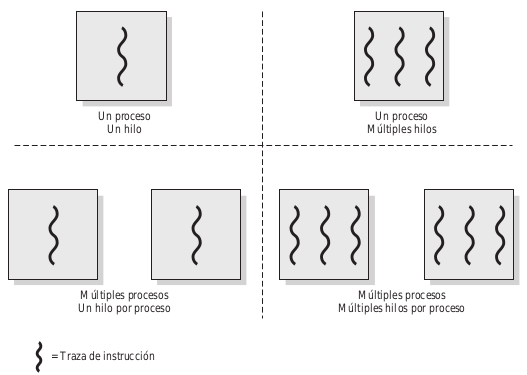
\includegraphics[width=0.8\textwidth, scale=1]{tema_2_figura17.png}
					\end{figure}
					
					En un entorno multihilo, un proceso se define como la unidad de asignación de recursos y una unidad de protección. Se asocian con procesos los siguientes:
					
					\begin{itemize}
					\item Un espacio de direcciones virtuales que soporta la imagen del proceso
					\item Acceso protegido a procesadores, otros procesos, archivos y recursos de E/S
					
					Dentro de un procesos puede haber uno o más hilos ejecutando, cada uno con:
					
					\item Un estado de ejecución por hilo.
					\item Un contexto de hilo que se almacena cuando no está en ejecución; una fomra de ver un hilo es como un contador de programa independiente dentro de un proceso.
					\item Una pila de ejecución.
					\item Por cada hilo, espacio de almacenamiento para variables locales.
					\item Acceso a la memoria y recursos de su proceso, compartido con todos los hilos de su mismo proceso.
					\end{itemize}
					
					En un modelo de procesos monohilo, la representación de un proceso incluye su PCB y el espacio de direcciones de usuario, además de las pilas de usuario y núcleo para gestionar el comportamiento de las llamadas/retornos en la ejecución de procesos. Mientras el proceso está ejecutando, los registros del procesador se controlan por ese proceso y, cuando el proceso no está ejecutando, se almacena el contenido de estos registros. En un entorno multihilo, sigue habiendo un único PCB y un espacio de direcciones de usuario asociado al proceso, pero ahora hay varias pilas separadas para cada hilo, así como un TCB que tiene los valores de registros, la prioridad, y otra información relativa al estado del hilo. \\
					
					De esta forma, todos los hilos de un proceso comparten el estado y los recursos del procesos, residen en el mismo espacio de direcciones y tienen acceso a los mismo datos. Cuando un hilo cambia determinados datos en memoria, otros hilos ven los resultados cuando acceden a estos. Si un hilo abre un archivo con permisos de lectura, los demás hilos del mismo proceso pueden también leer ese archivo. \\
					
					Los mayores beneficios de los hilos provienen de las consecuencias del rendimiento: 
					
					\begin{enumerate}
					\item Lleva mucho menos tiempo crear un hilo de un proceso existente que crear un proceso totalmente nuevo.
					\item Lleva menos tiempo finalizar un hilo que un proceso.
					\item Lleva menos tiempo cambiar entre dos hilos dentro del mismo proceso.
					\item Los hilos mejoran la eficiencia de la comunicación entre diferentes programas que están ejecutando. En la mayor parte de los SOs, la comunicación entre procesos independientes requiere la intervención del núcleo para proporcionar los mecanismo necesarios. Sin embargo, ya que los hilos de un proceso comparten memoria y archivos, se pueden comunicar sin necesidad de invocar al núcleo.
					\end{enumerate}
					
					Si se desea implementar una aplicación o función como un conjunto de unidades de ejecución relacionadas, es más eficiente hacer como conjunto de hilos que como conjunto de procesos independientes. \\
					
					A veces los hilos son también útiles en un solo procesador ya que ayudad a simplificar la estructura de programas que realizan varias funciones diferentes. \\
					
					Ejemplos de uso de hilos en un sistema de multiprocesamiento de un sólo usuario:
					
					\begin{itemize}
					\item \textbf{Trabajo en primer y segundo plano.} Por ejemplo, en un programa de hoja de cálculo, un hilo podría mostrar menús y leer la entrada de usuario, mientras otro hilo ejecuta los mandatos de usuario y actualiza la hoja de cálculo. Esta forma de trabajo a menudo incrementa la velocidad que se percibe de la aplicación, permitiendo al programa solicitar el siguiente mandato antes de que el mandato anterior esté completado.
					
					\item \textbf{Procesamineto asíncrono.} Los elementos asíncronos de un programa se pueden implementar como hilos. Por ejemplo, se puede diseñar un procesador de textos con protección contra un fallo de corriente que escriba el buffer de su memoria RAM a disco una vez por minuto. Se puede crear un hilo cuyo único trabajo sea crear una copia de seguridad periódicamente y que se planifique directamente a través del sistema operativo; no se necesita código adicional en el programa principal que proporcione control de tiempo o que coordine la entrada/salida.
					
					\item \textbf{Velocidad de ejecución.} Un proceso multihilo puede computar una serie de datos mientras que lee los siguientes de un dispositivo. En un sistema multiprocesador pueden estar ejecutando simultáneamente múltiples hilos de un mismo proceso. De esta forma, aunque un hilo pueda estar bloqueado por una operación de E/S mientras lee datos, otro hilo puede estar ejecutando.
					
					\item \textbf{Estructura modular de programas.} Los programas realizan diversas tareas o que tienen varias fuentes y destinos de entrada y salida, se pueden diseñar e implementar más fácilmente usando hilo.
					\end{itemize}
					
					En un sistema operativo que soporte hilos, la planificación y la activación se realizan a nivel de hilo; de aquí que la mayor parte de la información de estado relativa a la ejecución se mantenga en estructuras de datos a nivel de hilo. Existen, sin embargo, diversas acciones que afectan a todos los hilos de un proceso y que el SO debe gestionar al nivel de proceso. Suspender un proceso implica expulsar el espacio de direcciones de un proceso de memoria principal para dejar hueco a otro espacio de direcciones de otro proceso. Ya que todos los hilos de un proceso comparten el mismo espacio de direcciones, todos los hilos se suspenden al mismo tiempo. De forma similar, la finalización de un proceso finaliza todos los hilos de este.
				\subsubsection{Funcionalidades de los hilos}
					Los hilos, al igual que los procesos, tienen estados de ejecución y se pueden sincronizar entre ellos. \\
					
					\textbf{Estados de los hilos.} Los estados de los hilos principales son: ejecutando, listo, bloqueado. Generalmente, no tiene sentido aplicar estados de suspensión a un hilo, ya que dichos estados son conceptos a nivel de proceso. En particular, si se expulsa un proceso, todos sus hilos se deben expulsar porque comparten el espacio de direcciones del proceso. \\
					
					Hay cuatro operaciones básicas relacionadas con los hilos que están asociadas al cambio de estado del hilo:
					
					\begin{itemize}
					\item \textbf{Creación.} Cuando se crea un nuevo proceso, también se crea un hilo de dicho proceso. Pos-
teriormente, un hilo del proceso puede crear otro hilo dentro del mismo proceso, proporcionando un puntero a las instrucciones y los argumentos para el nuevo hilo. Al nuevo hilo se le proporciona su propio registro de contexto y espacio de pila y se coloca en la cola de Listos. 
					\item \textbf{Bloqueo.} Cuando un hilo necesita esperar a un evento se bloquea, almacenando los registros de usuario, contador de programa y punteros de pila. El procesador puede pasar a ejecutar otro hilo de la cola de listo, dentro del mismo proceso o de otro proceso.
					\item \textbf{Desbloqueo.} Cuando sucede el evento por el que un hilo se bloquea, este pasa a la cola de listos.
					\item \textbf{Finalización.} Cuando se completa un hilo, se liberan su registro de contexto y pilas.
					\end{itemize}
					
					*(RPC es una técnica por la que los programas, que pueden ejecutar en diferentes máquinas, interactúan utilizando la sintaxis y la semántica de las llamadas a procedimiento. Tanto el programa llamante omo el llamado se comportan como si el otro estuviera en la misma máquina). \\
					
					En un uniprocesador, la multiprogramación permite el intercalado de múltiples hilos con múltiples procesos. La ejecución pasa de un hilo a otro cuando se bloquea el hilo actualmente en ejecución o su porción de tiempo se agota. \\
					\textbf{Sincronización de hilos.} Todos los hilos de un proceso comparten espacio de direcciones y otros recursos. Cualquier alteración de un recurso por cualquiera de los hilos, afecta al entorno del resto de los hilos del mismo procesos. Por tanto, es necesario sincronizar las actividades de los hilos para que no interfieran entre ellos o corrompan etructuras de datos. Los asuntos que surgen y las técnicas que se utilizan en la sincronización de hilos son , en general, los mismo que en la sincronización de procesos.
					
				\subsubsection{Hilos de nivel de usuario y de nivel de núcleo}
					Existen dos amplias categorías de implementacion de hilos: hilos de nivel de usuario (\textit{user-level threads, UTL}) e hilos de nivel de núcleo (\textit{kernel-level threads, KTL}). Los últimos son también conocidos como hilos soportados por el núcleo (\textit{kernel-supported threads}) o procesos ligeros (\textit{lightweight processes}).
					
					\textbf{Hilos de nivel de usuario.} En un entorno ULT puro, la aplicación gestiona todo el trabajo de los hilos y el núcleo no es conscientede la existencia de estos.
					
					\begin{figure}
					\caption{Hilos de nivel de usuario y de nivel de núcleo}
					\label{figura2.18:hilosUK}
					\centering
					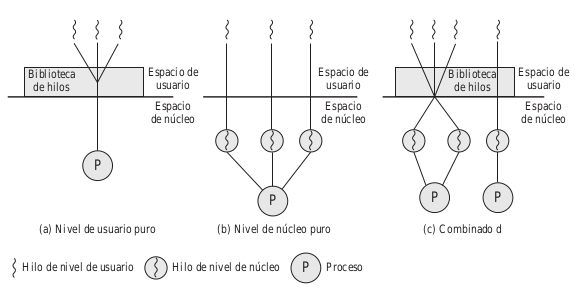
\includegraphics[width=1\textwidth, scale=1]{tema_2_figura18.png}
					\end{figure}
					
					Cualquier aplicación puede programarse para ser multihilo a través del uso de una biblioteca de hilos, que es un paquete de rutinas para la gestión de ULT. La biblioteca de hilos contiene código para la creación y destrucción de hilos, para paso de mensajes y datos entre hilos, para planificar la ejecución de hilos, y para guardar y restaurar el contexto de los hilos. \\
					
					Por defecto, una aplicación comienza con un solo hilo y ejecutando en ese hilo. Esta aplicación y su hilo se localizan en un solo proceso gestionado por el núcleo. En cualquier momento que la aplicación esté ejecutando (el proceso está en estado Ejecutando), la aplicación puede crear un nuevo hilo a ejecutar dentro del mismo proceso. La creación se realiza llamando a la utilidad de creación en la biblioteca de hilos. Se pasa el control a esta utilidad a través de una llamada a procedimiento. La biblioteca de hilos crea una estructura de datos para el nuevo hilo y luego pasa el control a uno de los hilos de ese proceso que esté en estado listo, utilizando algún algoritmo de planificación. Cuando se pasa el
control a la biblioteca, se almacena el contexto del hilo actual, y cuando se pasa el control de la biblioteca al hilo, se recupera el contexto de ese hilo. El contexto tiene esencialmente el contenido de los registros del usuario, el contador que programa, y los punteros de pila. \\

					Todo lo anterior tiene lugar en el espacio de usuario y dentro de un único proceso. El núcleo no es consciente de esta actividad. El núcleo continúa planificando el proceso como una unidad y asigna al proceso un único estado. \\
					
					Ventajas del uso de UTL en lugar de KTL:
					
					\begin{enumerate}
					\item El cambio de hilo no requiere privilegiso de modo núcleo porque todas las estructuras de datos de gestión de hilos están en el espacio de direcciones de usuario de un solo proceso. Por consiguiente, el proceso no cambia a modo núcleo para realizar la gestion de hilos. Esto ahorra la sobrecarga de dos cambios de modos.
					\item La planificación puede especificarse por parte de la aplicación. Una aplicación se puede beneficiar de un simple algoritmo de planificación cíclico, mientras que otras se podría beneficiar de un algoritmo de planificación basado en prioridades. El algoritmo de planificación de puede hacer a medida sin tocar el planificador del SO.
					\item Los UTL pueden ejecutar en cualquier SO. No se necesita cambio en el nuevo núcleo para dar soporte a los UTL. La biblioteca de los hilos es un conjunto de utilidades a nivel de aplicación que comparten todas las aplicaciones.
					\end{enumerate}
					
					Desventajas de los ULT en comparación con los KLT:
					
					\begin{enumerate}
					\item En un SO típico muchas llamadas al sistema son bloqueantes. Como resultado, cuando un UTL realiza una llamada al sistema, no sólo bloquea el hilo, sino que bloquea todos los hilos del procesos. \\
					 \item En una estrategia pura UTL, una aplicación multihilo no puede sacar ventaja del multiproceso. El núcleo asigna el proceso a un solo procesador al mismo tiempo. Por consiguiente, en un determinado momento sólo se puede ejecutar un hilo de proceso. En efecto, tenemos multiprogramación a nivel de aplicación de un solo proceso. Aunque esta multiprogramación puede dar lugar a una mejora significativa de la velocidad de la aplicacion, hay aplicaciones que se podrían beneficiar de la habilidad de ejecutar porciones de código concurrente.
					\end{enumerate}
					
					Hay forma de afrontar estos dos problemas. Por ejemplo, ambos puede superarse escribiendo una aplicación de múltiples procesos en lugar de múltiples hilos. Esto elimina la ventaja de los hilos. \\
					
					Otra forma de solucionar el problema de hilos que se bloquean es una técnica denominada \textit{jacketing}(revestimiento). El objetivo es convertir una llamada al sistema bloqueante en una no bloqueante. Por ejemplo, en lugar de llamar a una rutina del sistema de E/S, unhilo puede llamar a una rutina \textit{jackert} de E/S a nivel de aplicación. Con esta rutina \textit{jacket}, el código verifica si el dispositivo E/S está ocupado. Si lo está, el dispositivo pasa a bloqueado y pasa el control a otro hilo. Cuando lo recupera, chequea de nuevo el dispositivo. \\
					
					\textbf{Hilos a nivel de núcleo.} En un entorno KTL puro, el núcleo gestiona todo el trabajo de gestión de hilos. No hay código de gestión de hilos en la aplicación, solamente una interfaz de aplicación (API) para acceder a las utilidades del núcleo. \\
					
					Cualquier apliación puede programarse para ser multihilo. Todos los hilos de una aplicación se mantienen en un solo proceso. El núcleo mantiene información de contexto del proceso como una entidad y de los hilos individuales del proceso. La planificación realizada por el núcleo se realiza a nivel de hilo. Este enfoque resuelve los dos principales inconvenientes del enfoque ULT. Primero, el núcleo puede planificar simultáneamente múltiples hilos de un solo proceso en múltiples procesadores. Segundo, si se bloquea un hilo de un proceso, el núcleo puede planificar otro hilo del mismo proceso. Otra ventaja del enfoque KLT es que las rutinas del núcleo pueden ser en sí mismas multihilo. \\
					
					La principal desventaja del enfoque KLT en comparación con el enfoque ULT es que la transferencia de control de un hilo a otro del mismo proceso requiere un cambio de modo al núcleo. En cuanto a rendimiento los ULT con mas rápidos que los KLT y ambos son mucho más rápidos que los procesos. \\
					
					De esta forma, mientras que hay una ganancia significativa entre el uso de multihilos KLT en comparación con procesos de un solo hilo, hay una ganancia significativa adicional por el uso de ULT. Sin embargo, depende de la naturaleza de la aplicación involucrada que nos podamos beneficiar o no de la ganancia adicional. Si la mayor parte de los cambios de hilo en una aplicación requieren acceso al modo núcleo, el esquema basado en ULT no sería tan superior al esquema basado en KLT. \\
					
					\textbf{Enfoques combinados.}.(véase \ref{figura2.18:hilosUK}). Algunos SOs proporcionan utilidades combinadas ULT/KLT. En un sistema combinado, la creación de hilos se realiza por completo en el espacio de usuario, como la mayor parte de la planificación y sincronización de hilos dentro de una aplicación. Los múltiples ULT de una palicación se asocian en un número (menor o igual) de KLT. El programador debe ajustar el número de KLT para una máquina y aplicación en particular par lograr los mejores resultados posibles. \\
					
					En los enfoques combinados, múltiples hilos de la misma aplicación pueden ejecutar en paralelo en múltiples procesadores, y una llamada al sistema bloqueante no necesita bloquear el proceso completo. Si el sistema está bien diseñado, este enfoque debería combinar las ventajas de ambos enfoques puros, minimizando las desventajas.
				
				\subsubsection{Otras configuraciones}
					Los conceptos de asignación de recursos y unidades de activación an sido tradicionalmente relacionados con el concepto de proceso; esto es, como una relación 1:1 entre los hislos y procesos. Recientemente, ha habido mucho interŕes en proporcionar múltiples hilos dentro de un solo proceso, lo que es una relación muchos-a-uno. \\
					
					\begin{figure}
					\caption{Relación entre hilos y procesos}
					\label{figura2.19:rel-hilos-procesos}
					\centering
					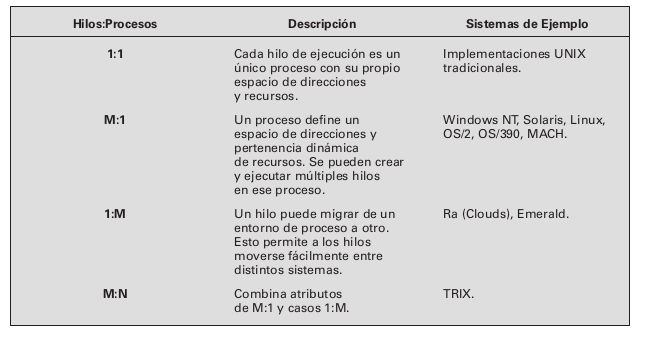
\includegraphics[width=1\textwidth, scale=1]{tema_2_figura19.png}
					\end{figure}
					
					\textbf{Relación muchos-a-muchos.} En TRIX, existen los conceptos de dominio de hilo. Un dominio es una entidad estática, que consiste en un espacio de direcciones y <<puertos>> a través de los cuales se pueden enviar y recibir mensajes. Un hilo es una ruta de ejecución, con una pila de ejecución, estado del procesador e información de planificación. \\
					
					Al igual que en el enfoque multihilo, múltiples hilos podrían ejecutar en un solo dominio. Sin embargo, también es posible realizar la actividad de usuario o ejecutar aplicaciones en múltiples dominios. En este caso hay un hilo que se puede mover entre dominios. \\
					
					El uso de un solo hilo en múltiples dominios está motivado por el deseo de proporcionar herramientas de estructuración al programador. \\
					
					\textbf{Relación uno-a-muchos.} En el campo de los SO distribuidos, ha habido interés en el concepto de un hilo como una entidad que se puede mover entre espacios de direcciones. \\
					
					Desde el punto de vista el usuarion, un hilo en Clouds es una unidad de actividad. Un proceso es un espacio de direcciones virtual con un bloque de control de proceso asociado. Una vez creado, un hilo comienza ejecutando en un proceso a través de la invocación de un punto de entrada de un programa en ese proceso. Los hilos se pueden moveer de un espacio de direcciones a otro, incluso fuera de los límites de la máquina. Según se mueve el hilo, debe llevarse determinada información con él (controlador de terminal, parámetros globales y guía de planificación). \\
					
					El enfoque de Clouds proporciona una forma eficiente de aislar a los usuarios y programadores de los detalles del entorno distribuido. La actividad de usuario puede ser representada como un solo hilo, y el movimiento de ese hilo entre máquinas puede ser gestionado por el SO gracias a información relativa al sistema.
					
		\section{Planificación uniprocesador.}
			\subsection{Tipos de planificación del procesador}
				El objetivo de la planificación de procesos es asignar procesos a ser ejecutados por el prcesador o procesadores a lo largo del tiempo, de forma que se cumplan los objetivos del sistema tales como tiempo de respuesta, rendimiento y eficiencia del procesador. En muchos sistemas, esta actividad de planificaión se divide en tres funciones: planificación a largo-,medio- y corto plazo.
				
				\begin{figure}
				\caption{Tipos de planificación}
				\label{figura2.20:tiposplanifición}
				\centering
				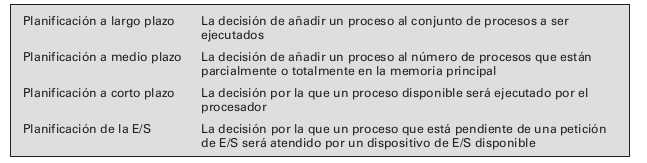
\includegraphics[width=1\textwidth, scale=1]{tema_2_figura20.png}
				\end{figure}
				
				La planificación a largo plazo se realiza cuando se crea un nuevo proceso. Hay que decidir si se añade un nuevo proceso al conjunto de los que están activos actualmente. La planificación a medio plazo es parte de la función de intercambio (swapping function). Hay que decidir si se añade un proceso a los que están al menos parcialmente en memoria y que, por tanto, están disponibles para su ejecución. La planificación a corto plazo conlleva decidir cuál de los procesos listos para ejecutar es ejecutado.
				
				\begin{figure}
				\caption{Planificación y transiciones de estado de los procesos}
				\label{figura2.21:planificación y transiciones}
				\centering
				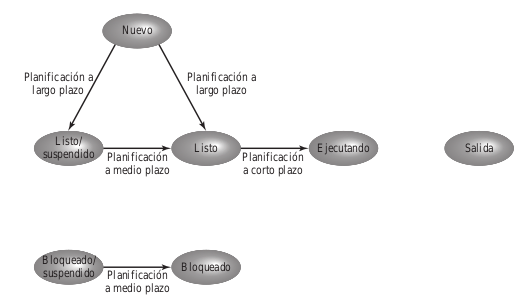
\includegraphics[width=1\textwidth, scale=1]{tema_2_figura21.png}
				\end{figure}
				
				La planificación afecta al rendimiento del sistema porque determina qué proceso esperará y qué proceso progresará. Fundamentalmente, la planificación es un problema de manejo de colas para minimizar el retardo en la cola y para optimizar el rendimiento en un entorno de colas.
				
			\subsubsection{Planificación a largo plazo}
				El planificador a largo plazo determina qué programas se admiten en el sistema para su procesamiento. De esta forma, se controla el grado de multiprogramación. Una vez admitido, un trabajo o programa de usuario se convierte en proceso y se añada a la cola del planificador a corto plazo. En algunos sistemas, un proceso de reciente creación comienza en la zona de intercambio, en cuyo caso se añaden a la cola del planificador a medio plazo. \\
				
				En un sistema por lotes, o en la parte de lotes de un SO de propósito general, los nuevos trabajos enviados se manda al disco y se mantienen en una cola de lotes. El planificador a largo plazo creará procesos desde la cola siempre que pueda. En este caso el planificador toma dos decisiones, la primera, el planificador debe decidir cuándo el SO puede coger uno o más procesos adicionales, la segundo, el planificador debe decidir qué trabajo o trabajos se aceptan y son convertidos en procesos. \\
				
				La decisión de cuándo crear un nuevo proceso se toma dependiendo del grado de multiprogramación deseado. Cuanto mayor sea el número de procesos creados, menor será el porcentaje de tiempo en que cada proceso se pueda ejecutar. De esta forma, el planificador a largo plazo puede limitar el grado de multiprogramación a fin de proporcionar un servicio satisfactorio al actual conjunto de procesos. Cada vez que termine un trabajo, el planificador puede decidir añadir uno o más nuevos trabajos. Además, si la fracción de tiempo que el procesador está ocioso excede un determinado valor, se puede invocar al planificador a largo plazo. \\
				
				La decisión de qué trabajo admitir, puede basarse en un sencillo FCFS(\textit{first come first service}), o puede ser una herramienta para gestionar el rendimiento del sistema. El criterio utilizado puede incluir prioridad, tiempo estimado de ejecución y los requisitos de E/S. Además, la decisión puede ser tomada dependiendo de los recursos de E/S que vayan a ser utilizados, de forma que se intente equilibrar el uso de la E/S. \\
				
				Para los programas interactivos en un sistema de tiempo compartido, la petición de la creación de un proceso, puede estar generada por un usuario intentando conectarse al sistema. Los usuarios de tiempo compartido no se sitúan simplemente en una cola hasta que el sistema los pueda aceptar. Más exactamente, el sistema operativo aceptará a todos los usuarios autorizados hasta que el sistema se sature. La saturación se estima utilizando ciertas medidas prefijadas del sistema. Llegado a este punto, una petición de conexión se encontrará con un mensaje indicando que el sistema está completo y el usuario debería reintentarlo más tarde. 
				
			\subsubsection{Planificación a medio plazo}
				La planificación a medio plazo es parte de la función de intercambio (\textit{swapping}). Con frecuencia, la decisión de intercambio se basa en la necesidad de gestionar el grado de multiprogramación. En un sistema que no utiliza la memoria virtual, la gestión de la memoria es también otro aspecto a tener en cuenta. De esta forma, la decisión de meter un proceso en la memoria, tendrá en cuenta las necesidades de memoria de los procesos que están fuera de la mismo.
			
			\subsubsection{Planificación a corto plazo}
				En términos de frecuencia de ejecución, el planificador a largo plazo ejecuta con relativamente poca frecuencia y toma la decisión de grano grueso de admitir o no un nuevo proceso y qué admitir. El planificador a medio plazo se ejecuta más frecuentemente para tomar decisiones de intercambio. El planificador a corto plazo, ejecuta muchos más frecuentemente y tomas las decisiones de grano fino sobre qué proceso ejecutar el siguiente. \\
				
				El planificador a corto plazo se invoca siempre que ocurre un evento que puede conllevar el bloqueo del proceso actual y que puede proporcionar la oportunidad de expulsar al proceso actualmente en ejecución por otro. Ejemplos de estos eventos:
				\begin{itemize}
				\item Interrupciones de reloj
				\item Interrupciones de E/S
				\item Llamadas al sistema
				\item Señales
				\end{itemize}
				
		\subsection{Algotirmos de planificación}
			\subsubsection{Criterios de la planificación a corto plazo}
				El objetivo principal de la planificación a corto plazo es asignar tiempo de procesador de tal forma
que se optimicen uno o más aspectos del comportamiento del sistema. Generalmente, se establece un conjunto de criterios con los que se pueden evaluar varias políticas de lanificación. \\
				
				Los criterios utilizados habitualmente se pueden categorizar en dos dimensiones. Primero, se puede hacer distinción entre criterios orientados al usuario y orientados al sistema. Los criterios orientados al usuario están relacionados con el comportamiento del sistema tal y como lo percibe un usuario individual o un proceso. \\
				
				Otros criterios son los relacionados con el sistema. Es decir, la atención se centra en el uso efectivo y eficiente del procesador. Un ejemplo es el rendimiento (\textit{throughput}), que es la tasa con que los procesos se finalizan. Esta medida es valiosa en relación al sistema y es algo que nos gustaría maximizar. Sin embargo, no se centra en los servicios proporcionados al usuario. De esta forma, el rendimiento incumbe al administrador del sistema pero no a los usuarios. \\
				
				Mientras que los criterios orientados al usuario son importantes en prácticamente todos los sistemas, los criterios orientados al sistema son generalmente menos importantes en sistemas de un solo usuario. En sistemas de un solo usuario, probablemente no es tan importante lograr una alta utilización del procesador o un alto rendimiento como que la respuesta del sistema a las aplicaciones del usuario sea aceptable.\\
				
				También es posible clasificar los criterios dependiendo de si están o no relacionado con las prestaciones. Los criterios relacionados con las prestaciones son cuantitativos y generalmente pueden ser medidos. Algunos ejemplos son el tiempo de respuesta y el rendimiento. Los criterios que no están relacionados con las prestaciones, o son cualitativos por naturaleza, o no pueden ser medidos y analizados (ej. previsibilidad). Nos gustaría que el servicio proporcionado a los usuarios tuviera las mismas características a lo largo del tiempo, independientemente de otros trabajos que se estén realizando en el sistema. Hasta cierto punto este criterio puede ser medido calculando las discrepancias en función de la carga de trabajo. Sin embargo, esta medida no es tan directa como medir el rendimiento o el tiempo de respuesta como una función de la carga de trabajo. \\
				
				\begin{figure}
				\centering
				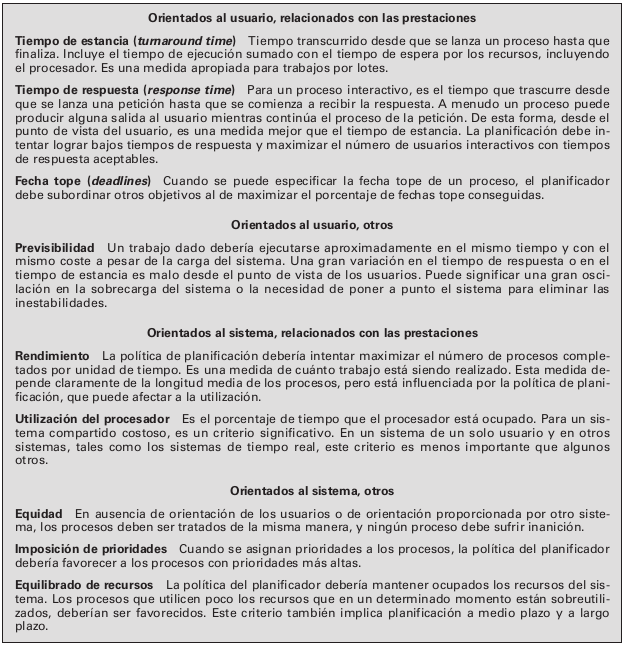
\includegraphics[width=1.2\textwidth, scale=1]{tema_2_figura22.png}
				\end{figure}
				
				En la mayor parte de los SOs interactivos, ya sean de un solo usuario o de tiempo compartido, un adecuado tiempo de respuesta es un requisito crítico.
				
			\subsubsection{El uso de prioridades}
				En muchos sistemas, a cada proceso se le asigna una prioridad y el planificador siempre elegirá un proceso de prioridad mayor sobre un proceso de prioridad menor.  \\
				
				Un problema de los esquemas de planificación con prioridades es que los procesos con prioridad más baja pueden sufrir inanición. Esto sucederá si hay siempre un conjunto de procesos de mayor prioridad listos para ejecutar. Si este comportamiento no es deseable, la prioridad de un proceso puede cambiar su antiguedad o histórico de ejecución.
				
			\subsubsection{Políticas de planficación alternativas}
				\textbf{La función de selección} determina qué proceso, entre los listos, se selecciona para ejecución. La función puede estar basade en prioridades, requisitos sobres los recursos, o las característica del procesos. En el último caso, hay tres medidas cuantitativas: \\
			
				w = tiempo usado en el sistema hasta este momento, esperando o ejecutando
				
				e = tiempo usado en ejecución hasta este momento
				
				s = tiempo de servicio requerido por el proceso, inlcuyendo e; generalmente, esta cantidad debe ser estimada o proporcionada por el usuario.
				
				El \textbf{modo de decisión} especifica los instantes de tiempo en que se ejecuta la función de selección. Hay dos categorías generales:
				
				\begin{itemize}
				\item \textbf{Sin expulsión (\textit{nonpreemptive}).} En este caso, una vez que el proceso está en el estado ejecutando, continúa ejecutando hasta que (a) termina o (b) se bloquea para esperar E/S o para solicitar algún servicio al SO.
				\item \textbf{Con expulsión (\textit{preemptive}).} Un proceso ejecutando en un determinado momento puede ser interrumpido y pasado al estado listo por el SO. La decisión de expulsar puede ser tomada cuando llega un nuevo proceso, cuando llega una interrupción que pasa un proceso de bloqueado a listo, o periódicamente, basándose en las interrupciones del reloj.
				\end{itemize}
				
				Las políticas expulsivas tienen mayor sobrecarga que las no expulsivas, pero pueden proporcionar mejor servicio a la población total de procesos, ya que previenen que cualquier proceso pueda monopolizar el procesador durante mucho tiempo. Además, el coste de la expulsión puede resultar relativamente bajo a través de la utilización de mecanismos eficientes de cambios de proceso (tanta ayuda del hardware como sea posible) y proporcionando una gran cantidad de memoria principal para dejar un alto porcentaje de programas en la memoria principal. \\
				
				Podemos pensar en estos procesos como trabajos por lotes, con un tiempo de servicio igual al tiempo de ejecución requerido. También los podemos considerar como procesos en curso que requieren un uso alternativo del procesador y de la E/S de forma repetitiva. En este último caso, los tiempos de servicio representan el tiempo de procesador requerido en un ciclo. En cualquier caso, en términos de un modelo de colas, esta cantidad se corresponde con el tiempo de servicio. \\
				
				Primero, se determina el tiempo de finalización de cada proceso. De esta forma, se puede determinar el timepo de estancia. En términos del modelo de colas, el \textbf{tiempo de estancia}(\textit{turnaround time} - TAT) es el tiempo de residencia o tiempo total que un elemento está en el sistema. Algo más útil es el tiempo de estancia normalizado, que es tasa del tiempo de estancia y tiempo de servicio. Este valor indica el retardo relativo experimentado por un proceso. Así, mayor sea el tiempo de ejecución, mayor será el valor absoluto del retardo que se puede tolerar. El menor valor posible para esta tasa es 1,0 ; valores mayores corresponden a un servicio de nivel menor. \\
				
				\textbf{Primero en llegar, primero en servirse (\textit{first-come-first-served}).} La directiva de planificación más sencilla es FCFS, también conocida como primero que entra primero que sale (FIFO) o como un sistema de colas estricto. En el momento en que un proceso pasa al estado de listo, se une a la cola de listos. Cuando el proceso actualmente en ejecución deja de ejecutar, se selecciona para ejecutar el proceso que ha estado más tiempo en la cola de listos.  \\
				
				Este tipo de planificación funciona bien para procesos largos pero no tanto para cortos. Se puede dar el caso en el que a la cola de listos llegue un proceso corto después de uno largo, como consecuencia su tiempo de estancia será demasiado grande. \\
				
				Otro problema de FCFS es que tiende a favorecer procesos limitados por el procesador sobre los limitados por la E/S. Considere que hay una colección de procesos, uno de los cuales está limitado por el procesador y un número de procesos limitados por la E/S. Cuando el limitado por el procesador está ejecutando, el resto debe esperar. Algunos de estos estarán en colas de E/S(bloqueados) pero se pueden mover a la cola de listos mientras que el proceso limitado por el procesador sigue ejecutando. En este punto, la mayor parte de los dispositivos de E/S pueden estar ociosos, incluso aunque exista trabajo potencial que puedan hacer. Cuando el proceso actual en ejecución deja el estado ejecutando, los procesos listos pasarán a ejecutando y se volverán a bloquear en un evento de E/S. Si el proceso limitado por el procesador está también bloqueado, el procesador se quedará ocioso. De esta manera, FCFS puede conllevar usos ineficientes del procesador y de los dispositivos de E/S. \\
				
				FCFS no es una alternativa atractiva por sí misma en un sistema uniprocesador. Sin embargo, a menudo se combina con esquemas de prioridades para proporcionar una planificación eficaz. De esta forma, el planificador puede mantener varias colas, una por cada nivel de prioridad, y despachar dentro de cada cola usando el primero en llegar, primero en servirse. \\
				
				\textbf{Turno rotatorio (\textit{round robin})} Una forma directa de reducir el castigo que tienen los trabajos con FCFS es la utilización de expulsión basándose en reloj. La  política más sencilla es la del turno rotatorio. Se genera una interrupción de reloj cada cierto intervalo de tiempo. Cuando sucede la interrupción, el proceso actual en ejecución se sitúa en la cola de listos, y se selecciona el siguiente trabajo según la política FCFS. Esta técnica es conocida como (\textit{time slicing}) se le da una rodaja de tiempo antes de ser expulsado. \\
				
				Con la planificación en turno rotatorio, el tema clave de diseño es la longitud del quantum de tiempo, o rodaja, a ser utilizada. Si el quantum es muy pequeño, el proceso se moverá por el sistema relativamente rápido. Por otra parte, existe una sobrecarga de procesamiento debido al manejo de la interrupción de reloj y por las funciones de planificación y activación. De esta forma, se deben evitar los quantums de tiempo muy pequeños. Una buena idea es que el quantum de tiempo debe ser ligeramente mayor que el tiempo requerido para una interacción o una función típica del proceso. \\
				
				La planificación en turno rotatorio es particularmente efectiva en sistemas de tiempo compartido de propósito general o en sistemas de procesamiento transaccional. Una desventaja de la planificación en turno rotatorio es que trata de forma desigual a los procesos limitados por el procesador y a los procesos limitados por la E/S. Generalmente, un proceso limitado por la E/S tiene ráfagas de procesador más cortas (cantidad de tiempo de ejecución utilizada entre operaciones de E/S) que los procesos limitados por el procesador. Si hay una mezcla de los dos tipos de procesos, sucederá lo siguiente: un proceso limitado por la E/S utiliza el procesador durante un periodo corto y luego se bloquea; espera a que complete la operación de E/S y a continuación se une a la cola de listos. Por otra parte, un proceso limitado por el procesador generalmente utiliza la rodaja de tiempo completa mientras ejecuta e inmediatamente vuelve a la cola de listos. De esta forma, los procesos limitados por el procesador tienden a recibir una rodaja no equitativa de tiempo de procesador, lo que conlleva un mal rendimiento de los procesos limitados por la E/S, uso ineficiente de los recursos de E/S y un incremento en la varianza del tiempo de respuesta. \\
				
				Una solución a este problema sería la disposición de una cola auxiliar FCFS a la que se mueven los procesos después de estar bloqueados en una E/S. Cuando se va a tomar una decisión de activación, los procesos en la cola auxiliar tienen preferencia sobre los de la cola de listos. Cuando se activa un proceso de la cola auxiliar, éste ejecuta por un tiempo no superior a una rodaja de tiempo, menos tiempo total que ha estado ejecutando desde que no está en la cola principal de listos.  \\
				
				\textbf{Primero el proceso más corto (\textit{shortest process next}).} Otro enfoque para reducir el sesgo a favor de los procesos largos inherente al FCFS es la política SPN. Es una política no expulsiva en la que se selecciona al proceso con el timepo de procesamineto más corto esperado. De esta forma un proceso corto se situará a la cabeza de la cola, por delante de los procesos más largos. \\
				
				El rendimiento global se mejora significativamente en términos del tiempo de respuesta. Sin embargo, se incrementa la variabilidad de los tiempos de respuesta, especialmente para los procesos más largos, y de esta forma se reduce la predecibilidad.  \\
				
				Un problema de la política SPN es la necesidad de saber, o al menos estimar, el tiempo de procesamiento requerido por cada proceso. Para trabajos por lotes, el sistema puede requerir que el programador estime el valor y se lo proporcione al SO. Si la estimación del programador es mucho menor que el tiempo actual de ejecución, el sistema podría abortar el trabajo. En un entorno de producción, ejecutan frecuentemente los mismos trabajo y, por tanto, se pueden recoger estadísticas. Para procesos interactivos, el SO podría guardar una media del tiempo de ejecución de cada <<ráfaga>> de cada proceso. La forma más sencida de cálculo sería:
				
				\begin{equation}
				S_{n+1} = \frac{1}{n}\sum_{i=1}^{n}T_{i}
				\end{equation}
				
				donde, 
				
				$T_{i}$ = Tiempo de ejecución del procesador para la instancia i-ésima de este proceso
				
				$S_{i}$ = valor predicho para la instancia i-ésima
				
				$S_{1}$ = valor predicho para la primera instancia; no calculado.
				
				Para evitar volver a calcular la suma completa cada vez, podemos reescribir la ecuación como 
				
				\begin{equation}
				S_{n+1}=\frac{1}{n}T_{n}+\frac{n-1}{n}S_{n}
				\end{equation}
				
				Esta fórmula otorga el mismo peso a cada instancia. Así, nos gustaría otorgar mayor peso a las instancias más recientes, ya que hay más probabilidades de que reflejen comportamientos futuros. El promedio exponencial es una técnica común de predecir valores futura basándose en una serie de tiempos pasados:
				
				 \begin{equation}
				 S_{n+1}=\alpha T_{n} + (1-\alpha)S_{n}
				 \end{equation}
				 
				 donde $\alpha$ es un factor de multiplicación constantes (0 < $\alpha$ < 1) que determina el peso relativo dado a las observaciones más recientes en relación a las antiguas observaciones. A través del uso de un valor constante $\alpha$, independientemente del número de observaciones pasadas, todos los valores pasados se consideran, pero los más distantes tienen menor peso. \\
				 
				 La ventaja de utilizar un valor de $\alpha$ cercano a 1 es que el promedio reflejará un cambio rápido en las cantidades observadas. Las desventaja es que si hay un cambio brusco en los valores observados y luego vuelven a su valor medio anterior, el uso de un valor alto de $\alpha$ puede dar lugar a oscilaciones en el promedio. \\
				 
				 Un riesgo con SPN es la posibilidad de inanición para los procesos más largos, si hay una llegada constante de procesos más cortos. Por otra parte, aunque SPN reduce la predisposición a favor de los trabajos más largos, no es desable para un entorno de tiempo compartido o de procesamiento transaccional por la carencia de expulsión. \\
				 
				 \textbf{Menor tiempo restante (\textit{shortest remaining time first}).} La política del menor tiempo restante (SRTF) es una versión expulsiva de SPN. En este caso, el planificador siempre escoge el proceso que tiene el menor tiempo restante esperado. Cuando un nuevo proceso se une a la cola de listos, podría tener un tiempo menor que el proceso actualmente en ejecución. Por tanto, el planificador podría expulsar al proceso actual cuando llega un nuevo proceso. Al igual que con SPN, el planificador debe tener una estimación del tiempo proceso para realizar la función seleccionada, y existe riesgo de inanición para los procesos más largos. \\
				 
				 SRT no tiene el sesgo en favor de los procesos largos que se puede encontrar en FCFS. A diferencia del turno rotatoria, no se generan interrupciones adicionales, reduciéndose la sobrecarga. Por otro parte, se deben almacenar los tiempo de servicio transcurridos, generando sobrecarga. SRT debería mejorar los tiempos de estancia de SPN, porque a un trabajo corto se le da preferncia sobre un largo. \\
				 
				 \textbf{Retroalimentación (\textit{feedback}).} Si no es posible averiguar el tiempo de servicio de varios procesos, SPN, SRTF no se pueden utilizar. Otra forma de establecer una prefencia para los trabajos más cortor es penalizar a los trabajos que han estado ejecutando más tiempo. En otras palabras, si no podemos basar en el tiempo de ejecución restante, nos podemos basar en el tiempo de ejecución utilizado hasta el momento. \\
				 
				 La forma de hacerlo es, la planificación se realiza con expulsión(por rodajas de tiempo), y se utiliza un mecanismo de prioridades dinámico. Cuando un proceso entra al sistema se le da máxima prioridad. Después de su primera expulsión, cuando vuelve al estado de Listo se le reduce la prioridad. Cada vez que es expulsado, se le coloca en la siguiente cola con menor prioridad. Un proceso corto se completará de forma rápidad, sin llegar a migrar muy lejos en la jerarquía de colas de listos. Un proceso largo irá degradándose gradualmente. De esta forma, se favores a los procesos nuevos más cortos sobre los viejos y largos. Dentro de cada cola, excepto en la cola de menor prioridad, se utiliza un mecanismo FCFS. Una vez en la cola de menor prioridad, un procesos no puede descender más, por lo que es devuelvo a esta cola repetidas veces mediante una política Round-Robin. \\
				 
				 Este enfoque se conoce como retroalimentación multinivel, ya que el SO adjudica el procesador a un proceso y, cuando se bloquea o es expulsado, lo vuelve a situar en una de las varias colas de prioridad. \\
				 
				 Un problema de este esquema es que el tiempo de estancia de procesos más largos se puede alargar de forma alarmante. De hecho, puede ocurrir inanición si están entrando nuevos trabajos frecuentemente en el sistema. Para compensar este problema, podemos variar los teimpos de expulsión de cada cola (ej, la cola de más prioridad tiene una rodaja de tiempo, la siguiente dos y así sucesivamente, de forma que en la i-ésima cola se tienen $2^i$ rodajas de tiempo antes de ser expulsado). \\
				 
				 Incluso asignando rodajas de tiempo mayores a las colas de menor prioridad, un proceso grande puede sufrir inanición. Una posible solución es promover a los procesos a colas de mayor prioridad una vez superen el umbral de inanición.
				 
		\section{Planificación multiprocesador y tiempo real}
			\subsection{Panificación multiprocesador}
				\subsubsection{Aspectos de diseño}
					En un multiprocesador la planificación involucra tres aspectos interrelacionados:
					
					\begin{itemize}
					\item La asignación de procesos a procesadores.
					\item El uso de multiprogramación en cada procesador individual.
					\item La activación del proceso, propiamente dicha.
					\end{itemize}
					
					\textbf{Asignación de procesos a procesadores.} Si se asume que la arquitectura multiprocesador es uniforma, en el sentido de que ningún procesador tienen ventaja física particular con respecto al acceso a memoria principal o a dispositivos de E/S, entonces el enfoque más simple de la planificación consiste en tratar cada proceso como un recurso colectivo y asignar procesos a procesadores por demanda. Sugre la cuestión de si la asignación debería ser estática o dinámica. \\
					
					Si un proceso se vincula permanentemente a un procesador desde su activación hasta que concluye, entonces se mantiene una cola a corto plazo dedicada por cada procesador. Una ventaja de esta estrategia es que puede haber menos sobrecarga en la función de planificación, dado que la asignación a un procesador se realiza una vez y para siempre. Asimismo, el uso de procesadores dedicados permite una estrategia conocida como planificación de grupo o pandilla, como se verá más adelante. \\
					
					Una desventaja de la asignación estática es que un procesador puede estar ocioso, con su cola vacía, mientras otro tiene trabajo acumulado. Para evitar esta situación, puede utilizarse una cola común. Todos los procesos van a una cola global y son planificados sobre cualquier procesador disponible. Así, a lo largo de la vida de un proceso, puede ser ejecutado en diferentes procesadores en diferentes momentos. En una arquitectura de memoria compartida fuertemente acoplada, la información de contexto de todos los procesos estará disponible para todos los procesadores, y por lo tanto el coste de planificación de un proceso será independiente de la identidad del procesador sobre cual se planifica. Otra opción más, es el balance dinámico de carga, en el que los hilos se mueven de una cola de un procesador a la cola de otro procesador. \\
					
					Independientemente de cómo los procesos se vinculan a los procesadores, se necesita alguna manera de asignar procesos a procesadores. Se han venido usando dos enfoques: maestro/esclavo y camaradas. Con la arquitectura maestro/esclavo, ciertas funciones clave del núcleo del sistema operativo ejecutan siempre en un procesador concreto. Los otros procesadores sólo pueden ejecutar programas de usuario. El maestro es responsable de la planificación de trabajos. Una vez que el proceso está activo, si el esclavo necesita un servicio, debe enviar una solicitud al maestro y esperar a que el servicio se realice. Este enfoque es bastante simple y sólo requiere mejorar un poco un SO monoprocesador multiprogramado. La resolución de conflictos se simplifica porque un procesador tiene todo el control de la memoria y de los recursos de E/S. Desventajas:
					
					\begin{itemize}
					\item Un fallo  en el maestro hace que falle todo el sistema.
					\item El maestro puede llegar a ser un cuello de botella para el rendimiento de todo el sistema.
					\end{itemize}
					
					En la arquitectura camaradas, el núcleo puede ser ejecutado en cualquier procesador, y cada procesador se auto-planifica desde la colección de procesos disponibles. Este enfoque complica el sistema operativo. El sistema operativo debe asegurar que dos procesadores no escogen el mismo proceso y que los procesos no se extravían por ninguna razón. Deben emplearse técnicas para resolver y sin cronizar la competencia en la demanda de recursos. \\
					
					Por supuesto, hay una gama de opciones entre estos dos extremos. Un enfoque es tener un subconjunto de los procesadores dedicado a procesar el núcleo en vez de uno solo. Otro enfoque es simplemente gestionar las diferentes necesidades entre procesos del núcleo y otros procesos sobre la base de la prioridad y la historia de ejecución. \\
					
					\textbf{El uso de la multiprogramación en procesadores individuales.} En los multiprocesadores tradicionales, que tratan con sincronizaciones de grano grueso o independientes, está claro que cada procesador individual debe ser capaz de cambiar entre varios procesos para conseguir una alta utilización y por tanto un mejor rendimiento. No obstante, para aplicaciones de grano medio ejecutando en un multiprocesador con muchos procesadores, la situación está menos clara. Cuando hay muchos procesadores disponibles, conseguir que cada procesador esté ocupado tanto tiempo como sea posible deja de ser lo más importante. En cambio, la
preocupación es proporcionar el mejor rendimiento, medio, de las aplicaciones. Una aplicación que consista en varios hilos, puede ejecutar con dificultad a menos que todos sus hilos estén dispuestos a ejecutar simultáneamente. \\
					
					\textbf{Activación de procesos.} El último aspecto de diseño relacionado con la planificación multiprocesador, es la elección real del proceso a ejecutar. Hemos visto que en un monoprocesador multiprogramado, el uso de prioridades o de sofisticados algoritmos de planificación basodos en el uso pasado, pueden mejorar el rendimiento frente a la estrategia FCFS. Cuando consideramos multiprocesadores, estas complejidades pueden ser innecesarias o incluso contraproducentes, y un enfoque más simple puede ser más eficaz con menos sobrecarga. En el caso de la planificación de hilos, entran en juego nuevos aspectos que pueden ser más importatnes que las prioridades o las historias de ejecución. 
					
				\subsubsection{Planificación de procesos}
					En los sistemas multiprocesador más tradicionales, los procesos no se vinculan a los procesadores. En cambio hay una única cola para todos los procesadores o, si se utiliza algún tipo de esquema basado en prioridades, hay múltiples colas basadas en prioridad, alimentando a un único colectivo de procesadores. En cualquier caso, el sistema puede verse como una arquitectura de colas multiservidor. \\
					
					La conclusión general es que la plnaificación específica es muchos menos importante con dos procesadores que con uno. Debería ser evidente que sta conclusión es incluso más fuerte a medidad que el número de procesadores crece. Así, la disciplina FCFS con un esquema estático de prioridades puede ser suficiente en un sistema multiprocesador. 
					
				\subsubsection{Planificación de hilos}
					Como hemos visto, con los hilos, el concepto de ejecución se separa del resto de la definición de un proceso. Una aplicación puede ser implementada como un conjunto de hilos, que cooperan y ejecutan de forma concurrente en el mismo espacio de direcciones. \\
					
					En un monoprocesador, los hilos pueden usarse como una ayuda a la estructuración de programas y para solapar E/S con el procesamiento. Dada la mínima penalización por realizar un camibo de hilo comparada con un cambio de proceso, los beneficios se obtienen con poco coste. \\
					
					Sin embargo, el poder completo de los hilos se vuelve evidente en un sistema multiprocesador. En este entorno, los hilos pueden explotar paralelismo real dentro de una aplicación. Si los hilos de una aplicación están ejecutando simultáneamente en procesadores separados, es posible una mejora drástica de sus prestaciones. Sin embargo, puede demostrarse que para aplicaciones que necesitan una interacción significativa entre hilos (paralelismo de grano medio), pequeñas diferencias en la gestión y planificación de hilos pueden dar lugar a un impacto significativo en las prestaciones. \\
					
					En las propuestas para la planificación multiprocesador de hilso destacan cuatro enfoques:
					
					\begin{itemize}
					\item \textbf{Compartición de carga.} Los procesos no se asignan a un procesador particular. Se mantiene una cola global de hilos listo, y cada procesador, cuando está ocioso, selecciona un hilo de la cola. El término \textbf{compartición de carga} se utiliza para distinguir esta estrategia de los esquemas de balanceo de carga en los que los trabajos se asignan de manera más permanente.
					\item  \textbf{Planificación en pandilla.} Un conjunto de hilos relacionados que se planifica para ejecutar sobre un conjunto de procesadores al mismo tiempo, en relación uno-a-uno.
					\item \textbf{Asignación de procesador dedicado.} Esto es lo opuesto al enfoque de compartición de carga y proporciona una planificación implícita definida por la asignación de hilos a procesadores. Cada proceso ocupa un número de procesadores igual al número de hilos en el programa, durante toda la ejecución del mismo. Cuando el programa termina, los procesadores regresan al parque general para la posible asignación de otro programa.
					 \item \textbf{Planificación dinámica.} El número de hilos de un proceso puede cambiar durante el curso de su ejecución.
					\end{itemize}
					
\section{Jerarquía de memoria}
	\subsection{Jerarquía de memoria y conceptos sobre cachés}
		La pregunata sobre cuánta debe ser su capacidad es algo que no tiene limite. Si se dispone de una determinada capcaidad probablementese desarrollarán aplicaciones que la usarán. Para alcanzar un redimiento máximo, la memoria debe ser capaz de mantener el rimto del procesador. Es decir, según el procesador va ejecutando instrucciones, no debería haber pausas esperando a que estén disponibles las instrucciones o los operandos. Por último, para un sistema práctico, el coste de la memoria debe ser razonable en relación con los otros componentes. \\
		
		Hay un compromiso entre las tres caracterísitcas fundamentales de la memoria: coste, capacidad y tiempo de acceso. En todo espectro de tecnologías se cumplen las siguientes realicones:
		
		\begin{itemize}
		\item Cuanto menor tiempo de acceso, mayor coste por bit.
		\item Cuanta mayor capacidad, menor coste por bit
		\item Cuanta mayor capacidad, menor velocidad de acceso.
		\end{itemize}
		
		La solución a este dilema es no basasrse en un único componente de memoria o en una sola tecnología, sino emplear una \textbf{jerarquía de memoria}. En la figura \ref{jerarquia de memoria} se muestra un esquema de la jerarquía de memoria. Según se desciende en al jerarquía ocurre lo siguiente:
		
		\begin{itemize}
		\item Disminución del coste por bit
		\item Aumento de la capacidad.
		\item Aumento del tiempo de acceso
		\item Disminución de la frecuencia de acceso a la memoria por parte del procesador.
		\end{itemize}
		
		\begin{figure}
		\centering
		\caption{Jeraquía de memoria}
		\label{jerarquia de memoria}
		\includegraphics[width=0.8\textwidth,scale=1]{tema_3_figura1.png}
		\end{figure}
		
		Por tanto las memoria más rápidas, caras y pequeñas se complementan con memorias más lentas, baratas y grandes. La clave del éxito es el último acceso: la disminución de la frecuencia de acceso. \\
		
		La validez de la condición (d) está basada en un principio conocido como la \textit{proximidad de referencias}. Durante el curso de ejecución de un programa, las referencias de memoria del procesador, tanto a instrucciones como a datos, tienden a agruparse. Los programa contienen habitualmente diversos bucles iterativos y subrutinas. Una vez que se inicia un bucle o una subrutina, hay referencias repetidas a un pequeño conjunto de instrucciones. Del mimso modo, las operaciones con tablas y vectores involucran accesos a conjuntos agrupados de bytes de datos. En un perido de tiempo largo, las agrupaciones que se están usando van cambiando, pero en un periodo corto, el procesador está principalmente trabajando con grupos fijos de referencias a memoria. \\
		
		Por consiguiente, es posible organizar los datos a través de la jerarquía de memoria de manera que el porcentaje de accesos a cada nivel sucesivamente más bajo es considerablemente menor que al nivel inferiro. \\
		
		El tipo de memoria más rápida, pequeña y costosa consiste en los registros internos del procesador. Normalmente, un procesador contendrá unas pocas docenas de ese tipo de registros, aunque algunas máquinas contienen cientos de registros. Descendiendo dos niveles, está la memoria principal que es el sistema de memoria interna fundamental del computador. Cada posición de memoria principal tiene una única dirección. La mayoría de las instrucciones máquina hacen referencia a una o más direcciones de memoria principal. La memoria principal se amplía usualmente con caché, más pequeña y de mayor velocidad. La caché normalmente no es visible al programador, o incluso, al procesador. Se trata de un dispositivo que controla el movimiento de datos entre la memoria principal y los registros del procesador con objeto de mejorar el rendimiento. \\
		
		Las tres formas descritas de memoria son, normalmente, volátiles y emplean tecnoloǵia de semiconductores. El uso de tres niveles explota el hecho de que la memoria de semiconductores se presenta en diversos tipos, que se diferencian en velocidad y coste. Los datos se almacenan de forma más permanente en los dispositivos de almacenamiento masivo externos, de los cuales los más comunes son los discos dureos y los dispositivos extraíbles. La memoria no volátil externa se denomina también \textbf{memoria secundaria} o \textbf{memoria auxiliar}. Se usa para almacenar los ficheros de programas y datos, siendo usualmente visibles al programador sólo en términos de ficheros y registros, en contraposición a byte o palabras individuales. El disco se utiliza también para proporcionar una extensión de la memoria conocida como memoria virtual.  \\
		
		De hecho, se puede añadir niveles adicionales a la jerarquía por software. Por ejemplo, se puede utilizar una parte de la memoria principal como una zona de almacenamiento intermedio para guardar temporalmente datos que van a ser leídos del disco. Esta técnica, denominada a veces caché de disco, mejora el rendimiento de dos maneras:
		
		\begin{itemize}
		\item Las escrituras en el disco pueden agruparse. En vez de muchas transferencias de datos de pequeño tamaño, se producen unas pocas transferencias de gran tamaño. Esto mejora el rendimiento del disco y minimiza el grado de implicación del procesador.
		\item Un programa puede acceder a algunos datos destinados a ser escritos antes del siguiente volcado al disco. En ese caso, los datos se recuperan rápidamente de la caché software en vez de lentamente como ocurre cuando se accede a disco.
		\end{itemize}
		
	\subsection{Memoria caché}
		Aunque la memoria cache es invisible para el sistema operativo, interactúa con otros elementos del hardware de gestión de memoria. Además, muchos de los principios usados en los esquemas de memoria virtual son aplicables también a la caché. \\
		
		\subsubsection{Motivación}
			En todos los ciclos de instrucción, el procesador accede al menos una vez, para leer la instrucción, y con frecuencia, una o más veces adicionales, para leer y/o almacenar resultados. La velocidad a la que el procesador puede ejecutar instrucciones está claramente limitada por el tiempo de ciclo de memoria. Esta limitación ha sido de hecho un problema significativo debido a la persistente discrepancia entre la velocidad del procesador y la de la memoria principal; a lo largo de los años, la velocidad del procesador se ha incrementado constantemente de forma más rápida que la velocidad de acceso a la memoria. Idealmente, se debería construir la memoria principal con la misma tecnología que la de los registros del procesador, consiguiendo tiempos de ciclo de memoria comparables a los tiempos de ciclo del procesador. Esta estrategia siempre ha resultado demasiado costosa. La solución consiste en aprovecharse del principio de proximidad utilizando una memoria pequeña y rápida entre el procesador y la memoria principal, denominada caché. \\
			
		\subsubsection{Fundamentos de la cache}
			El propósito de la caché es proporcionar un tiempo de acceso a memoria próximo al de las memorias más rápidas disponibles, y al mismo tiempo, ofrecer un tamaño de memoria grande que tenga el precio de los tipos de memorias semiconductores menos costosas. Hay una memoria principal relativamente grande y lenta junto con una memoria cache más pequeña y rápida. La cache contiene una copia de una parte de la memoria principal. Cuando el procesador intenta leer un byte de la memoria, se hace una comprobación para determinar si el byte está en la caché. Si es así, se le entrega el byte al procesador. En caso contrario, se ele e introduce dentro de la cache un bloque de memoria principal, que consta de un cierto número fijo de bytes y, a constinuación, se le entrega el byte pedido al procesador. Debido al fenómeno de proximidad de referencias, cuando se lee e introduce dentro de la cache un bloque de datos para satisfacer una única referencia de memoria, es probable que muchas de las referencias a memoria en el futuro próximo correspondan con otros bytes del bloque. \\
			
		\subsubsection{Diseño de la caché}
			Se dividen en las siguientes categorías:
			\begin{itemize}
			\item Tamaño de la caché
			\item Tamaño del bloque
			\item Función de correspondencia
			\item Algoritmo de reemplazo
			\item Política de escritura
			\end{itemize}
			
			Se ha tratado ya el tema del \textbf{tamaño de la cache}, llegándose a la conclusión de que una cache de un tamaño razonablemente pequeño puede tener un impacto signifactivo sobre el rendimiento. Otro aspecto relacionado con la capacidad de la caché es el tamaño del bloque, la unidad de datos que se intercambia entre la caché y la memoria principal. Según el tamaño del bloque se incrementa desde muy pequeño a tamaños mayores, al principio la tasa de aciertos aumentará debido al principio de proximidad: la alta probabilidad de que accedan en el futuro inmediato a los datos que están en la proximidad de una palabra a la que se ha hecho referencia. Según se incrementa el tamaño de blque, se llevan a la cache más datos útiles. Sin embargo, la tasa de aciertos comenzará a decerecer cuando el tamaño del bloque siga creciendo, ya que la probabilidad de volver a usar los datos recientemente leídos se hace menor que la de utilizar nuevamente los datos que se van a expulsar de la caché para dejar sitio al nuevo bloque. \\
			
			\begin{figure}
			\centering
			\caption{Operación de lectura de caché}
			\label{3.2: operación de lectura de cahce}
			\includegraphics[width=0.8\textwidth, scale=1]{tema_3_figura2.png}
			\end{figure}
			
			Cuando se lee e incluye un nuevo bloque de datos en la caché, la \textbf{función de correspondencia} determina que posición de la caché ocupará el bloque. Existen dos restricciones que afectan al diseño de la función de correspondencia. \\
			
			En primer lugar, cuando se introduce un bloque en la caché, se puede tener que reemplazar otro. Sería deseable hacer esto de manera que se minimizara la probabilidad de que se remplazase un bloque que se necesitara en el futuro inmediato. Cuanto más flexible es la función de correspondencia, mayor grado de libertad a la hora de diseñar un algoritmo de emplazo que maximice la tasa de aciertos. En segundo lugar, cuanto más flexible es la función de correspondencia, más compleja es la circuitería requerida para buscar en la cache y determinar si un bloque dado está allí. \\
			
			El \textbf{algoritmo de remplazo} selecciona, dentro de las restricciones de la función de correspondencia, qué bloque remplazar cuando un nuevo bloque va a cargarse en la cache y ésta tiene todos los huecos llenso con otros bloques. Sería deseable remplazar el bloque que menos probablemente se va a necesitar en el futuro inmediato. Aunque es imposible identificar tal bloque, una estrategia razonablemente eficiente es remplazar el bloque que ha estado en la caché durante más tiempo sin haberse producido ninguna referencia a él. Esta política se denomina el algorimto del \textit{menos recientemente usado (Least Recently Used}, LRU). Se necesitan mecanismos de hardware para identificar el bloque menos recientemente usado. \\
			
			Si se altera el contenido de un bloque en la cache, es necesario volverlo a escribir en la memoria principal antes de remplazarlo. La \textbf{política de escritura} dicta cuando tiene lugar la operación de escritura de memoria. Una alternativa es que la escritura se produzca cada vez que se actualiza el bloque. Otra opción es que la escritura se realice sólo cuando se remplaza el bloque. La última estrategia minimiza las operaciones de escritura en memoria pero deja la memoria principal temporalmente en un estado obsoleto. Esto puede interferir con el modo de operación de un multiprocesador y con el acceso directo a memoria realizado por los módulos hardware de E/S.
			
	\subsection{Hardware y estructuras de control}
		Comparanado la paginación sencilla y la segmentación sencilla, por un lado, tenemos una distinción entre particionamiento estático y dinámico, y por otro, tenemos los fundamentos de la gestión de memoria. Las dos características de la paginación y la segmentción son:
		
		\begin{itemize}
		\item  Todas las referencias a la memoria dentro de un proceso se realizan a direcciones lógicas, que se traducen dinámicamente en direcciones físicas durante la ejecución. Esto significa que un proceso puede ser llevado y traído a memoria de forma que ocupe diferentes regiones de la memoria principal en distintos instantes de tiempo de su ejecución.
		
		\item Un proceso puede dividirse en varias porciones (páginas o segmentos) y estas porciones no tienen que estar localizadas en la memoria de forma contigua durante la ejecución. La combinación de la traducción de direcciones dinámicas en ejecución y el uso de una tabla de páginas o segmentos lo permite.
		\end{itemize}
		
		Si las dos características anteriores se dan, entonces es necesario que todas las páginas o todos los segmentos de un proceso se encuentren en memoria principal durante la ejecución. Si la porción (segmento o página), en la que se encuentra la siguiente instrucción a buscar está y si la porción donde se encuentra la siguiente dirección de datos que se va a acceder también está, al menos la siguiente instrucción se podrá ejecutar. \\
		
		Supongamos que se tiene que traer un nuevo proceso de memoria. El SO comienza trayendo únicamente una o dos porciones, que incluye la porción inicial del programa y la porción inicial de datos sobre la cual acceden las primeras instrucciones. Esta parte del proceso que se encuentra realmente en la memoria principal para, cualquier instante de tiempo, se denomina \textbf{conjunto residente} del proceso. Cuando el proceso está ejecutándose, las cosas ocurren de forma suave mientras que todas las referencias a la memoria se encuentren dentro del conjunto residente. Usando una tabla de segmentos o páginas, el procesador siempre es capaz de determinar si esto es así o no. Si el procesador encuentra una dirección lógica que no se enecuentra en la memoria principal, generará una interrupción indicando un fallo de acceso a la memoria. El sistema operativo coloca al proceso interrupido en un estado bloqueado y toma el control. Para que la ejecución de este proceso pueda reanudarse más adelante, el sistema operativo necesita traer a la memoria principal la porción del proceso que contiene la dirección lógica que ha causado el fallo de acceso. El SO realiza una petición de E/S, una lectura a disco. Después de realizar la petición, el sistema operativo puede activar otro proceso que se ejecute mientras el disco realiza la operación de E/S. Una vez que la porción solicitada se ha traído a la memoria principal, una nueva interrupción de E/S se lanza, dando control de nuevo al sistema operativo, que coloca al proceso afectado de nuevo en el estado de Listo. \\
		
		\begin{enumerate}
		\item \textbf{Pueden mantenerse un mayor número de procesos en memoria principal.} Debido a que sólo vamos a cargar algunas de las porciones de los procesos a ejecutar, existe espacio para más procesos. Esto nos lleva a una utilización más eficiente del procesador porque es más probable que haya al menos uno o más de los numerosos procesos que se encuentre en el estado Listo, en un instante de tiempo concreto.
		\item \textbf{Un proceso puede ser mayor que toda la memoria principal.} Se puede superar una de las restricciones fundamentales de la programación. Sin el esquema que hemos estado discutiendo, un programador debe estar realmente atento a cuánta memoria está disponible. Si el prgrama que está escribiendo es demasiado grande, el programador debe buscar el modo de estructurar el programa en fragmentos que pueden cargarse de forma separada con un tipo de superposición (\textit{overlay}). Con la memoria virtual basada en paginación o segmentación, este trabajo se delega al sistema operativo y al hardware. En lo que concierne al programador, él está trabajando con una memoria enorme, con un tamaño asociado al almacenamiento de disco. El sistema operativo automáticamente carga porciones de un proceso en la memoria principal cuando éstas se necesitan.
		\end{enumerate}
		
		Debido a que un proceso ejecuta sólo en la memoria principal, esta memoria se denomina \textbf{memoria real}. Pero el programador o el usuario perciben una memoria potencialmente mucho más grande (\textbf{memoria virtual}). La memoria virtual permite una multiprogramación muy efectiva que libera al usuario de las restricciones excesivamente fuertes de la memoria principal.
		
		\begin{figure}
		\caption{Características de la segmentación y la paginación}
		\label{figura3.3:paginación y segmentación}
		\centering
		\includegraphics[width=1\textwidth, scale=1]{tema_3_figura3.png}
		\end{figure}
		
	\subsubsection{Proximidad y memoria virtual}
		Se va a considerar un programa de gran tamaño, consistente en un programa largo más un gran número de vectores de datos. A lo largo de un corto periodo de tiempo, la ejecución se puede acotar a una pequeña sección del programa y al acceso a uno o dos vectores de datos únicamente. Si es así, sería verdaderamente un desperdicio cargar docenas de prociones de dicho proceso cuando sólo unas pocas porciones se usarán antes de que el programa se suspenda o mande a zona \textit{swap}. Se puede hacer un mejor uso de la memoria cargando únicamente unas pocas porciones. Entonces, si el programa salta a una destrucción o hace referencia a un dato que se encuentra en una porción de memoria que no está en la memoria principal, se disparará un fallo. Ésta indica al SO que debe conseguir la porción deseada. \\
		
		Así, en cualquier momento, sólo unas pocas porciones de cada proceso se encuentran en memoria, y por tanto se pueden mantener más procesos alojados en la misma. Además, se ahorra tiempo porque las porciones del proceso no usadas no se expulsarán de la memoria a \textit{swap} y de \textit{swap} a la memoria. Sin embargo, el SO debe ser inteligente a la hora de manejar este esquema. En estado estable, prácticamente toda la memoria principal se encontrará ocupada con porciones de procesos de forma que el procesado y el SO tengan acceso directo al mayor número posible de procesos. Así, cuando el SO traiga una porción de memoria debe expulsar otra. Si elimina una porción justo antes de que vaya a ser utilizada, deberá recuperar dicha proción de nuevo casi de forma inmediata. Un abuso de esto lleva a una condición denominada \textbf{trasiego(\textit{thrashing})}: el sistema consume la mayor parte del tiempo enviando y trayendo porciones de \textit{swap} en lugar de ejecutar instrucciones. En esencia, el sistema operativo trata de adivinar, en base a la historia reciente, qué porciones son menos probables de ser utilizadas en un futuro cercano. \\
		
		Este razonamiento se basa en la creencia del \textbf{principio de proximidad}. Éste indica que las referencias al programa y a los datos dentro de un proceso tienden a agruparse. Por tanto, se resume en que sólo unas pocas porciones del proceso se necesitarán a lo largo de un peeriodo de tiempo ordinario. También, es posible hacer suposiciones inteligentes sobre cuáles son las porcioens del proceso que se necesitarán en un futuro próximo, para evitar este trasiego. \\
		
		Para que la memoria resulte práctica y efectiva, se necesitan dos ingredientes. Primero, debe existir un soporte hardware para el esquema de paginación y/o segmentación. Segundo, el sistema operativo debe incluir código para gestionar el movimiento de páginas y/o segmentos entre la memoria secundaria y la memoria principal. \\
		
	\subsubsection{Paginación}
		El término \textit{memoriva virtual} se asocia habitualmente con sistemas que emplean paginación, a pesar de que la memoria virtual basada en segmentación también se utiliza. \\
		
		En la representación de la paginación sencilla, indicamos que cada proceso dispone de su propia tabla de páginas, y que todas las páginas se encuentran localizadas en la memoria principal. Cada entrada en la tabla de páginas consiste en un número de marco de la correspondiente página en la memoria princiapl. Para la memoria virtual basada en el esquema de paginación también se necesita una tabla de páginas. De nuevo, normalmente se asocia una única tabla de páginas a cada proceso.En este caso, sin enmbargo, las entradas de la tabla de páginas son más complejas. Debido a que sólo algunas de las páginas de proceso se encuentran en la memoria principal, se necesita que cada entrada de la tabla de páginas indique si la correspondiente páginas está presente (P) en memoria principal o no. Si el bit indica que la página está en memoria, la entrada también debe indicar el número de marco de dicha página. \\
		
		La entrada de la tabla de páginas incluye un bit de modificado (M), que indica si los contenidos de la correspondiente página han sido alterados desde que la página se cargó por última vez en la memoria principal. Si no había ningún cambio, no es necesario escribir la página cuando llegue el momento de reemplazarla por otra página en el marco de página que actualmente ocupa. Pueden existir también otros bit de control de estas entradas. Por ejemplo, si la protección y compartición se gestiona a nivel de página, se necesitarán también los bits para este propósito. \\
		
		\textbf{Estructura de la tabla de páginas.} El mecanismo básico de lectura de una palabra de la memoria implica la traducción de la dirección virtual, o lógica, consistente en un número de página y un desplazamiento a la dirección física, consistente en un número de marco y un desplazamiento, usando para ello la tabla de páginas. Debido a que la tabla de páginas es de longitud variable dependiendo del tamaño del proceso, no podemos suponer que se encuentra almacenada en los registros. En lugar de eso, debe encontrarse en la memoria principal para poder ser accedida. \\
		
 		Para resolver el problama de las tablas de páginas excesivamente grande, la mayoría de esquemas de memoria virtual almacenan las tablas de páginas también en memoria virtual, en lugar de en la real. Esto representa que las talbas de páginas están sujetas a paginación igual que cualquier otra página. Cuando un proceso está en ejecución, al menos parte de su tabla de paǵinas debe encontrarse en memoria, incluyendo la entrada de la tabla de páginas de la página actualmente en ejecución. Algunos procesadores utilizan un esquema de dos niveles para organizar las tablas de páginas de gran tamaño. En este esquema, existe un directorio de páginas en el cual cada entrada apuntaba a una tabla de páginas. De esta forma, si la extensión del directorio de páginas es X, y si la longitud máxima de un tabla de páginas es Y, entonces un proceso consistirá en hasta $X \geq Y$ páginas. Normalmente, la longitud máxima de la tabla de páginas se restringe para que sea igual a una página. \\
 		
 		\textbf{Tabla de páginas invertida.} Una desventaja del tipo de tablas de páginas que hemos visto es que su tamaño es proporcional al espacio de direcciones virtuales. \\
 		
 		Una estrategia alternativa al uso de tablas de páginas de uno varios niveles es el uso de la estructura de \textbf{tabla de páginas invertida}. 
		
		
								
\end{document}

